\chapter{Introduction to Languages and Automata}\label{chap:languagesautomaten}

Computer programs are central in the activity of the computer
scientist. Computer programs transform a given input into a desired
output. The input could be an electric pulse indicating a temperature
change, a character from the keyboard, another program, a database
\ldots The output could be a sequence of signals controlling some valves,
a new version of a document, an error message, the display of a
graph \ldots

From a practical point of view, the above examples are quite
different, but when we focus too much on the details, we miss a lot.
We can abstract away many details and focus on the essence: in every
example, there is a mapping from elements in an input domain to
elements in an output domain. These domains are always discrete, and
sometimes infinite. This means that from a theoretical point of view,
programs are just functions from (a part of) $\N$ to (a part of) $\N$.

In case the input domain is small, that function is not very
interesting: one could just build a table with all precomputed values,
and then the computation is just a simple lookup.\footnote{Tabulation
is an interesting dynamic implementation technique, whichever the
programming paradigm. Ask if you want to know more.}

In case the input domain is large, or not a priori known, then it is
impossible to tabulate the function, so it is better to assume the
input domain is infinite.

Now about the output domain: it needs to contain at least two values
to be interesting. These two elements could be {\em yes, no} and that
is enough to describe {\em decision problems}: you want to know
whether a given input has a certain property, e.g. {\em is this
program syntactically correct?} or {\em is this a good day to invest
time in FCS?} \footnote{Yes !}  \ldots

If the output domain contains more than two elements, but a finite
number of them, then one can easily compute the correct output by a
finite sequence of yes/no questions. Suppose you want to know which is
the best day of the week for investing time in FCS (the output domain
has 7 values), you could ask the following yes/no questions {\em is
Monday the best day for investing time in FCS?}, {\em is Tuesday the
best day for investing time in FCS?} \ldots So, it seems that of all
finite output domains, the only really interesting one has exactly two
values.

If the output domain is infinite, the function can not be reduced
easily to a finite sequence of functions with a finite output domain.

We can conclude that there exist only two kinds of interesting
functions. They have signature $\N \rightarrow\{yes, no\}$ and $\N \rightarrow \N$.

We focus for now on the first kind: it is easy to associate a certain
structure and semantics with the output domain, but the input domain
is very generic. $\N$ could indeed be replaced by any other countably
infinite set. Moreover, when we note down elements of $\N$, we can use
decimal digits: we form strings (sequences) of such digits. We could
have used another basis for the representation - binary, hexadecimal,
or even more exotic excess-3, \ldots These representations have something
in common: a finite set of symbols is used (we name it an alphabet), a
sequence of such symbols (we name it a string) has a unique meaning,
and one can concatenate strings.
%
Let $\Sigma$ denote a finite alphabet, and let $\Sigma^*$ denote all
finite sequences of symbols from $\Sigma$. Then we have just argued
that the interesting functions have signature $\Sigma^* \rightarrow
\{yes, no\}$. A function $F$ in this class is totally determined by the
set of strings $s$ for which $F(s) = yes$, so instead of studying such
functions, we can just as well study subsets $V$ of $\Sigma^*$
together with the associated question: {\em does a given s belong to
$V$}. It is important to understand that we are still considering the
same class of functions $\N \rightarrow\{yes, no\}$, but also that it
is often more natural and insightful to describe decision problems
starting from a particular $\Sigma^*$. Almost all of computability
theory uses this framework.

The second kind of functions - the ones with signature $\N \rightarrow
\N$ - are of course very important as well, but will not be the focus
in this course.


{\bf Selfie:}
\begin{itemize}
\item[]
The introduction simplifies matters, and makes assumptions that you
might disagree with, or that require a bit more argument ... Find {\em
holes} in the introduction, think of alternatives, argue in favor and
against ...

Describe a decision problem already known to you, but now by choosing
an alphabet $\Sigma$ and defining a subset $Sol$ of $\Sigma^*$ that is
the solution to the problem. Do that for different kinds of problems:
with numbers, words, graphs, ... Make sure to construct an example in
which $Sol$ is finite and one in which it is infinite. What happens if
you interchange $yes$ and $no$?

\end{itemize}

\section{What is a Language?}

The introduction gives the motivation for studying decision
problems. A decision problem corresponds to a subset of all strings
(or words) consisting of elements of a finite alphabet $\Sigma$. Any
such subset is a {\em language} over $\Sigma$.

\begin{definition}[String over an alphabet $\Sigma$]
A {\bf string} over an alphabet $\Sigma$ is a finite sequence of zero,
one or more elements of $\Sigma$.
\end{definition}

Clearly, if we put two strings $x$ and $y$ one after the other, we get
a new string denoted $xy$.

\begin{definition}[Language over an alphabet $\Sigma$]
A {\bf language} over an alphabet $\Sigma$ is a set of (finite)
strings over $\Sigma$.
\end{definition}

A language can be finite or infinite. If the language $L$ is infinite,
is it countably infinite?\footnote{If you do not remember what that
means, now is the time to look it up}

In order to identify a language, one must give a description for every
element of the language, and that description should not fit any
string not in the language. E.g. the language of odd numbers (over the
alphabet of decimal digits), or the set of strings ending on
1,3,5,7,9. Another example: the English words rhyming with automata.

The description of a language is preferably finite, even if the
language itself is infinite.

The description of the language can {\em often} be used to check whether a
given string belongs to the language, and even to generate or
construct each element of the language. But be careful with the {\em
often}: we will need to get back to it.

If the description of a language is simple, we expect the language to
be simple, but we don't really have a good idea what {\em simple}
means here.

Here are some questions for you to think about: this course provides
you with material to answer them.

\begin{itemize}
\item
Do formalisms exist that can denote language descriptions?

\item
Does such a formalism allow to (automatically) derive testers and
generators for the language?

\item
Are there languages that do not fit the formalism?

\item
What is a good notion of testing/generating?

\item
Are some languages inherently easier to describe, test, generate?

\end{itemize}

And finally:

\begin{itemize}
\item[] Why should a computer scientist know all this?
\end{itemize}


\paragraph{Selfie:}
\begin{itemize}
\item[]

Can you use the description of the set of even numbers to generate all even numbers?

Same question but for the English words rhyming with automata.

Can you use them for testing?

Invent a new very extravagant language, give its description and use
it to test whether a given string belongs to it, and use it to
generate all strings belonging to the language.

Based on these examples, can you see a connection between the ease of
description, the testing and the generation?
\end{itemize}

%===============================================================================
\section{An Algebra of Languages}

An algebra (or algebraic structure) is a set with some internal
operations (often binary operations, but unary operations are also
common, and even operations with a larger arity). The set of languages
over the alphabet $\Sigma$ becomes an algebra by defining operations
like union, intersection, complement \ldots More concrete:
let $L_1$ and $L_2$ be two languages, then

\begin{itemize}
\item their union is a language: $L_1 \cup L_2$
\item their intersection is a language: $L_1 \cap L_2$
\item the complement is a language: $\overline{L_1}$
\end{itemize}

You can construct other operations on languages by composing the three
above, just like with any sets.

There is also a new way - not directly linked to set theory - to make
a new language out of two given languages: {\em concatenation}.

\begin{definition}[Concatenation of two languages]
Let $L_1$ and $L_2$ be two languages over the same alphabet $\Sigma$,
then we denote the concatenation of $L_1$ and $L_2$ by $L_1L_2$ and we
define: $L_1L_2 = \{xy | x \in L_1, y \in L_2\}$.
\end{definition}

When we concatenate three languages, we do not need brackets, because
clearly, concatenation is associative:
%
$(L_1L_2)L_3 = L_1(L_2L_3)$


Concatenating $L$ n times with itself is denoted by $L^n$.
$L^0$ contains only the empty string, and we denote that string by
$\epsilon$.

Finally, we also define an operation that allows to construct an
infinite language from a finite one:

\begin{definition}[$L^*$ - the Kleene {\bf star} of $L$]
$L^* = \cup_{n=0}^\infty L^n$
\end{definition}

As an abbreviation of $LL^*$ one uses $L^+$.


Now we have all this notation, we can say that $L$ is a language over
$\Sigma$ if $L \subseteq \Sigma^*$, or equivalently
%
$ L \in {\cal P}(\Sigma^*)$.

\paragraph{Selfie:} Define new operations on languages.

%===============================================================================
\section{Language Descriptions}

In maths, one uses the set notation, e.g.

\begin{example}
Let $\Sigma = \{x,y,z\}$:
\begin{itemize}
\item
$\Sigma^* = \{a_1a_2a_3...a_n|~a_i \in \Sigma, n \in \N \}$
\item
$L = \{a_1a_2a_3...a_n|~a_1 = y, n \in \N, \forall i > 1: a_i \in \Sigma\}$

or in words: L is the set of strings starting with y
\end{itemize}
\end{example}

Informal descriptions are possible as well, as long as they are not
ambiguous about membership.

\begin{example}
~~
\begin{itemize}
\item
$H(n) = \{P | P~is~a~Java~program~and~P~stops~after~at~most~~n~seconds~on~input~n\}$
\item
$Prime = \{n|n \in \N, n~is~prime\}$
\end{itemize}
\end{example}

While the last one is an informal description, it hides the formal
description of {\em prime}, so we could also have specified $Prime$ as

\hspace{1cm}$Prime = \{n|n \in \N, \forall i:1<i<n \rightarrow n~mod~i \neq 0\}$

This kind of description is OK for doing maths, but computer
scientists need a different formalism: it should (more easily) allow
to convert a description into a generator and a tester. For natural
languages, linguists have grammars: they describe the structure of a
sentence. Natural languages are very complicated, with lots of
exceptions to rules, and exceptions to exceptions \ldots It makes sense
to study classes of languages with a simpler structure. We aim
therefore at

\begin{itemize}
\item[]
a hierarchy of languages

\item[]
an accompanying hierarchy of description formalisms, or grammars

\item[]
an accompanying hierarchy of {\em test} and {\em generate} procedures

\end{itemize}

The hierarchy we study is named the {\em
Chomsky-hierarchy\footnote{Noam Chomsky}}. We start at the bottom of
this hierarchy, i.e. with the easiest languages.



%///////////////////////////////////////////////////////////////////////////////
\chapter{Regular Expressions and Regular Languages}

%===============================================================================
\section{Basic Definitions}

\begin{definition}[Regular Expression (RE) over an alphabet $\Sigma$] \label{defregexp}
E is a {\bf regular expression over alphabet $\Sigma$} if E has the form
\begin{itemize}
\item $\epsilon$
\item $\phi$
\item $a$ for $a \in \Sigma$
\item $(E_1E_2)$ for regular expressions $E_1$ and $E_2$ over $\Sigma$
\item $(E_1)^*$ for a regular expression $E_1$ over $\Sigma$
\item $(E_1 | E_2)$ for regular expressions $E_1$ and $E_2$ over $\Sigma$
\end{itemize}
\end{definition}

In this way, the set of regular expressions {\em RegExps} (over an
alphabet $\Sigma$) is defined inductively. It implies that something
that does not comply with the definition is not a regular expression,
and that every regular expression can be constructed using only the
rules above.
%
It is often implicitly clear which alphabet is used, and we often do
not mention it.
%
We use the brackets to avoid ambiguity: the brackets do not belong to
the alphabet.
%
In the next examples, $\Sigma = \{a,b,c\}$.

\begin{example}
Regular expressions over $\Sigma$:
\begin{itemize}
\item b
\item a($\epsilon$c)
\item $(((ab))^*c~|~(bc))$
\end{itemize}
\end{example}

Are we using too many brackets, too few? Why?

\begin{definition}
A regular expression E {\bf determines} a
language $L_E$ over its alphabet $\Sigma$ as follows:
\begin{itemize}
\item if E = a ($a \in \Sigma$) then $L_E = \{a\}$ (the language with
just one string, consisting of the character a)
\item if E = $\epsilon$ then $L_E = \{\epsilon\}$ (the empty string)
\item if E = $\phi$ then $L_E = \emptyset$ (the empty set)
\item if E = $(E_1E_2)$ then $L_E = L_{E_1}L_{E_2}$
\item if E = $(E_1)^*$ then $L_E = L_{E_1}^*$
\item if E = $(E_1 | E_2)$ then $L_E = L_{E_1} \cup L_{E_2}$
\end{itemize}
\end{definition}

This similarity between the structure of the regular expressions and
the structure of the languages they determine is not a coincidence,
and we can exploit it to use fewer brackets in regular expressions. We
just agree that $^*$ takes precedence over concatenation, which takes
precedence over union. Note also that concatenation is associative. So
we can agree that $L_{(((a)^*(b))c)} = L_{a^*bc}$. You should however
never say that the regular expression $(((a)^*(b))c)$ equals the
regular expression $a^*bc$: the correct wording is {\em the language
(determined by) $(((a)^*(b))c)$ equals the language (determined by)
$a^*bc$}.

\paragraph{Selfie:}
Formulate a verbal description of the languages determined by the REs
over $\{a,b\}$ below - the first one is an example:

\begin{itemize}
\item[]
$(ab)^*$: every $a$ is followed immediately by a $b$, and there are as
many $a$'s as $b$'s

$(aba)^*$

$(a|b)^*$

$(a|b)^*\phi$

$a \epsilon b$
\end{itemize}

\paragraph{Selfie:}
Prove the following statements, or give a counterexample:

\begin{itemize}
\item[]
if a regular expression E does not contain a $^*$, then $L_E$ is
finite

if a regular expression E contains a $^*$, then $L_E$ is infinite

$L_E \subseteq L_{(E|F)}$ for all RE's E and F

the set of regular expressions (over a given alphabet) is itself a
language (over which alphabet?)
\end{itemize}


\medskip

\begin{definition}[Regular Language]
A language determined by a regular expression is named a {\bf regular language}.
\end{definition}

We denote the set of regular languages by $RegLan$. Check which of the
formulas below make sense, and which are true.

\begin{enumerate}
\item $RegLan \subseteq \Sigma$
\item $RegLan \subseteq \Sigma^*$
\item $RegLan \subseteq {\cal P}(\Sigma)$
\item $RegLan \subseteq {\cal P}(\Sigma^*)$
\item $RegLan \subseteq {\cal P}({\cal P}(\Sigma^*))$
\item if $x \in RegLan$ then $x \in \Sigma$
\item if $x \in RegLan$ then $x \in \Sigma^*$
\item if $x \in RegLan$ then $x \in {\cal P}(\Sigma)$
\item if $x \in RegLan$ then $x \in {\cal P}(\Sigma^*)$
\item if $x \in RegLan$ and $y \in x$ then $y \in \Sigma$
\item if $x \in RegLan$ and $y \in x$ then $y \in \Sigma^*$
\item if $x \in RegLan$ and $y \in x$ then $y \in {\cal P}(\Sigma)$
\item if $x \in RegLan$ and $y \in x$ then $y \in {\cal P}(\Sigma^*)$
\end{enumerate}

\paragraph{Selfie:}

\begin{itemize}
\item[]
Is true that {\em for every regular language L, there exists a regular
expression E so that $L_E = L$}?


Is it clear that there exist languages that are NOT regular?

Is every finite language regular?

Is every infinite regular language countable?

Given a regular language, can you construct (one of) its regular
expression(s)?

For given string $s$ and regular expression $E$, can you
determine whether $s \in L_E$?

Can you generate all strings in $L_E$ once you have $E$?
\end{itemize}


\section{The Subalgebra of Regular Languages}

We denote the set of languages over alphabet $\Sigma$ by
$L_\Sigma$. It is an algebra for certain operations, and
%
$L_\Sigma = {\cal P}(\Sigma^*)$.

For $L_1, L_2 \in L_\Sigma$, we can consider the language $L_1L_2$
(concatenation), $L_1 \cup L_2$ (union), $L_1^*$ (repetition), and
$\overline{L_1}$ (complement). The result is always a member of
$L_\Sigma$. We say: $L_\Sigma$ is an algebra with (at least) four
internal operations.

Since $RegLan$ is a subset of $L_\Sigma$, it makes sense to ask whether
RegLan is a subalgebra of $L_\Sigma$. In other words: are the
operations internal to RegLan?

\paragraph{Selfie:} Formulate a theorem stating that RegLan is a
subalgebra of $L_\Sigma$ (for the four operations above), and prove it
in a constructive way, i.e. (for union) construct an E so that $L_E =
L_{E_1} \cup L_{E_2}$. Did you succeed for complement?


%===============================================================================
\section{Finite State Machines}

\newcommand{\atm}{\entrymodifiers={++[o][F-]}}
\newcommand{\accept}[1]{*++[o][F=]{#1}}

While regular expressions are a declarative way of describing (regular)
languages, 
Finite state machines (FSM) are a more operationl formalism. They
capture how to test and/or generate strings that belong
to a language.

In this chapter we focus on the particular class 
of FSMs known as deterministic finite state automata (DFAs).
We start with a
graphical representation of an FSM. The formal definition follows
later. Figure~\ref{fsa1} shows a first example of an {\em
DFA}  over
the alphabet $\{a,b,c\}$.

\begin{figure}[h]
\begin{equation*}
\atm\xymatrix{
*{} \ar[r] & q_0 \ar[r]^b\ar@(u,ul)_a\ar@/^/[d]_c & \accept{q_1}\ar@(u,ur)^{b}\ar[dl]_c\ar[d]_a \\
*{}        & q_2\ar[r]_c\ar@/^/[u]^{a,b} & \accept{q_3}\ar@(r,rd)^{a,b,c}
}
\end{equation*}
%  \begin{center}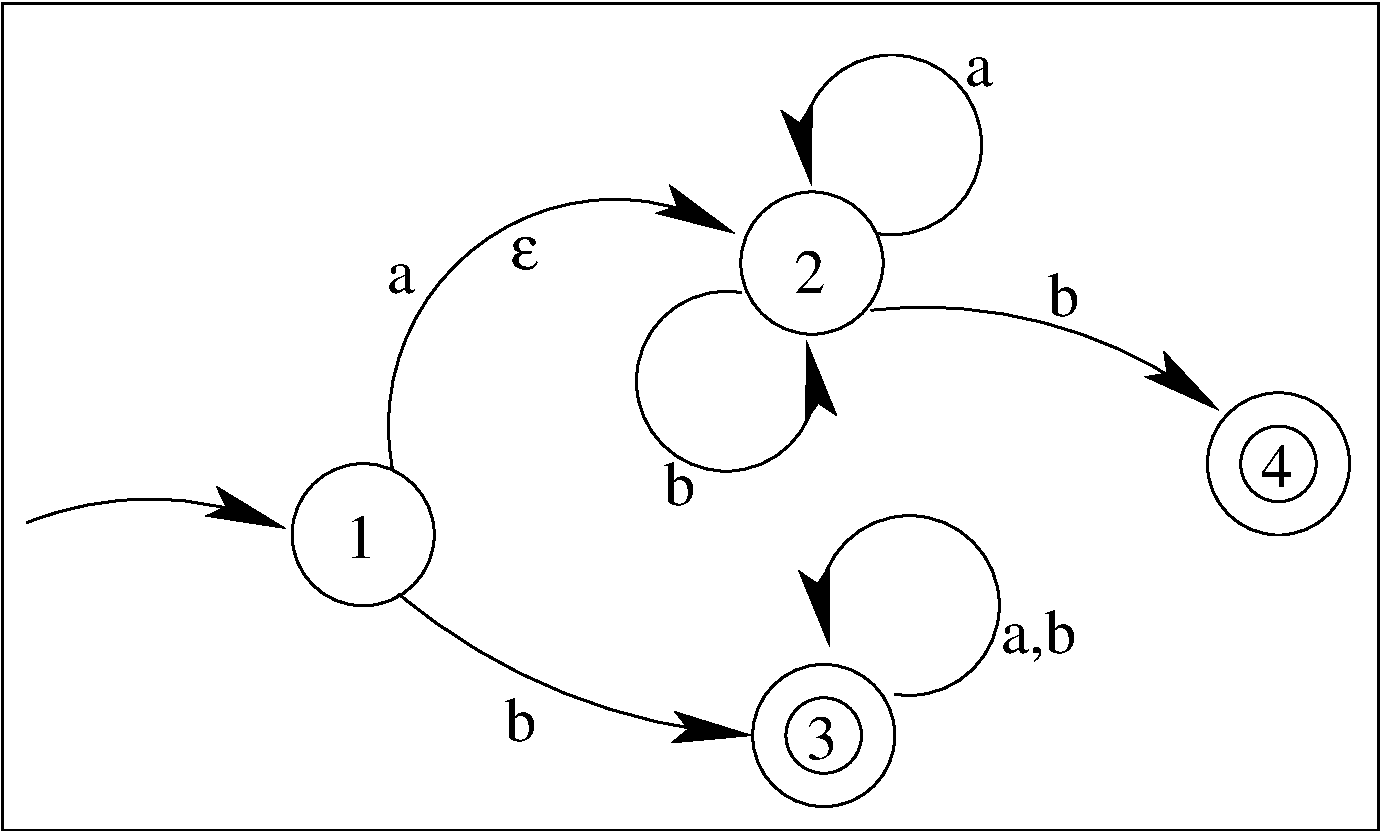
\includegraphics[%
%    width=0.5\linewidth,
%    keepaspectratio]{fsa1}\end{center}
\caption{A finite state machine\label{fsa1}}
\end{figure}

The most important characteristics are:

\begin{itemize}
\item we see a directed graph;
\item the vertices have a name (in this case a number) - the vertices
  are called {\em states};
\item there are two kinds of states: states with a double circle are
  called accepting states (sometimes also end states or final
  states)--the other states are non-acceping;
\item loops are allowed;
\item the edges are labelled with zero, one, or more symbols from the
  alphabet;
\item there is exactly one edge not starting from a vertex: the vertex
  in which it arrives is the start state.
\end{itemize}

We can use this graphical representation as follows:

\begin{enumerate}
\item you get a string $s$ over the alphabet (it is now your current
  string) and you start in the start state
\item you can now go from one state to the other along any given
  edge but you must pay a price for that: you spend from the beginning
  of your current string a symbol that appears on the edge (meaning
  that your string shortens)
  % ; in case the edge contains $\epsilon$,
  % you do not need to spend a symbol from your string
\item if you manage to arrive in an accepting state with an empty string,
  we say {\em the DFA accepts the initial string $s$}
\end{enumerate}

This constitues only an informal definition of which strings are
accepted by an DFA.

Here is a different use of the graphical representation:

\begin{enumerate}
\item start with an empty string in the start state: that is your
  current string
\item now follow any edges: add one of the symbols on the edge to your string; keep doing that
\item any time you arrive at an accepting state, you may say {\em this machine generates the current string}
\end{enumerate}



\paragraph{Selfie:} Answer the following questions:

\begin{itemize}
\item[]
does the DFA in Figure~\ref{fsa1} accept ac?

does the DFA in Figure~\ref{fsa1} accept bbb?

is there more than one way to accept bbb?

is it possible that you get stuck with bbb and what does that mean for bbb?

can you give some strings not accepted by this DFA?

% construct an NFA with a circuit - can you now get into an endless
% loop? is that a problem?

can you comment on {\em the set of strings generated by the DFA equals
  the set of strings accepted by the DFA} ?
\end{itemize}

\begin{definition}[A DFA M determines a language (informal)]
A language L is determined by the DFA M, if M accepts every string
from L, and no other strings. We denote this language by $L_M$.
\end{definition}

The alphabets of the DFA and the language do not need to be the same,
but it is convenient to assume they are.

\begin{definition}[Equivalence of DFAs]
Two DFAs are {\bf equivalent} if they determine the same language.
\end{definition}

The relation {\em DFA-equivalence} defines an equivalence relation on
DFAs: each equivalence class corresponds to one language.


\paragraph{Selfie:} think about the following

\begin{itemize}
\item[] there exists a procedure for deciding whether two given DFAs
  are equivalent

for each DFA there exists an equivalent one with at most one accepting
state

% for each NFA there exists an equivalent one in which {\em you can't
%   get stuck}
\end{itemize}

% We often need the set $\Sigma \cup \{\epsilon\}$: we abbreviate it by
% $\Sigma_\epsilon$.

\begin{definition}[Deterministic finite state automaton] \label{dfadef}
A {\bf deterministic finite state automaton} is a 5-tuple
$(Q,\Sigma,\delta,q_s,F)$ with
\begin{itemize}
\item Q a finite set of states
\item $\Sigma$ a finite alphabet
\item $\delta: Q \times \Sigma \to Q$ is the transition function
\item $q_s \in Q$ is the start state
\item $F \subseteq Q$: F is the set of accepting states
\end{itemize}
\end{definition}


The domain of $\delta$ in a DFA is $Q \times \Sigma$. It is useful to extend
$\delta$ to a function $\delta^*$ on the domain $Q \times \Sigma^*$ as follows:

\begin{eqnarray*}
\delta^*(q,\epsilon) & = & q \\
\delta^*(q,a \cdot w) & = & \delta^*(\delta(q,a),w)
\end{eqnarray*}

\paragraph{Selfie:}
\begin{itemize}
\item[]
Prove that $\delta^*(q,wa) = \delta(\delta^*(q,w),a)$ for $a \in
\Sigma$ and $w \in \Sigma^*$
\end{itemize}

%  \begin{definition}[Non-deterministic finite state automaton] \label{nfadef}
%  A {\bf non-deterministic finite state automaton} is a 5-tuple
%  $(Q,\Sigma,\delta,q_s,F)$ with
%  \begin{itemize}
%  \item Q a finite set of states
%  \item $\Sigma$ a finite alphabet
%  \item $\delta$ a transition function, i.e.
%  %
%  $\delta: Q \times \Sigma_\epsilon \rightarrow {\cal P}(Q)$
%  \item $q_s$ is the start state and an element of $Q$
%  \item $F \subseteq Q$: F is the set of final states
%  \end{itemize}
%  \end{definition}
%  
%  As you guessed by now: NFA is an acronym of {\em Non-deterministic Finite
%    Automaton}.


We formally define what it means for a string $s$ to be accepted by a
DFA.

%  \begin{definition}[A string accepted by an NFA] \label{defacceptnfa}
%  A string $s$ is accepted by an NFA
%  $(Q,\Sigma,\delta,q_s,F)$ if $s$ can be written as
%  $a_1a_2a_3...a_n$ with $a_i \in \Sigma_\epsilon$, and there
%  exist a sequence of states $t_1t_2t_2t_3...t_{n+1}$ so that
%  \begin{itemize}
%  \item $t_1 = q_s$
%  \item $t_{i+1} \in \delta(t_i,a_i)$
%  \item $t_{n+1} \in F$
%  \end{itemize}
%  \end{definition}

\begin{definition}[A string accepted by a DFA] \label{defacceptdfa}
A string $s$ is accepted by an DFA
$(Q,\Sigma,\delta,q_s,F)$ iff $\delta^*(q_s,w) \in F$.
\end{definition}

\paragraph{Selfie:}
\begin{itemize}
\item[]
You now have both an intuitive notion of acceptance by a DFA (through
its graphical representation) and a formal definition: make sure that
your intuition matches the definition.
\end{itemize}


%  Up to now, we have defined only non-deterministic automata: it is
%  possible that at a particular state, there is more than one outgoing
%  edge with the same symbol. This leaves a potential choice. But some of
%  those NFAs are deterministic: there is no choice. Such an automaton is
%  a DFA.

The next section shows the connection between regular expressions and
DFAs: we first construct a DFA from a RE so that $L_{RE} = L_{DFA}$,
and later we do the reverse. Together, this will prove that the two
formalisms are (in some sense) equivalent.


\subsection*{The Transition Table}

The $\delta$ of a DFA is a function with a finite domain. It can be
represented in the form of a table named the {\em transition table}:
it shows the transitions of the DFA. As an example,
here is the transition table for the DFA in Figure~\ref{fsa1}:

%\begin{table}[ht]
{\center
\begin{tabular}{|r|r||r|}
\hline
$Q$    & $\Sigma$           & $Q$ \\ \hline
$q_0$    & a                  & $q_0$       \\
$q_0$    & b                  & $q_1$       \\
$q_0$    & c                  & $q_2$       \\
$q_1$    & a                  & $q_3$       \\
$q_1$    & b                  & $q_1$       \\
$q_1$    & c                  & $q_2$       \\
$q_2$    & a                  & $q_0$       \\
$q_2$    & b                  & $q_0$       \\
$q_2$    & c                  & $q_3$       \\
$q_3$    & a                  & $q_3$       \\
$q_3$    & b                  & $q_3$       \\
$q_3$    & c                  & $q_3$       \\
\hline
\end{tabular}
% \caption{The transition table of the DFA in
% Figure~\ref{fsa1}} \label{transitietabel}
}
% \end{table}
%  %\begin{table}[ht]
%  {\center
%  \begin{tabular}{|r|r|r|}
%  \hline
%  $Q$    & $\Sigma_\epsilon$ &  ${\cal P}(Q)$ \\ \hline
%  1      & a                  &  $\{2\}$         \\
%  1      & b                  &  $\{3\}$         \\
%  1      & $\epsilon$         &  $\{2\}$         \\
%  2      & a                  &  $\{2\}$         \\
%  2      & b                  &  $\{2,4\}$         \\
%  3      & a                  &  $\{3\}$         \\
%  3      & b                  &  $\{3\}$         \\ \hline
%  2      & $\epsilon$         &  $\emptyset$         \\
%  3      & $\epsilon$         &  $\emptyset$         \\
%  4      & a                  &  $\emptyset$         \\
%  4      & b                  &  $\emptyset$         \\
%  4      & $\epsilon$         &  $\emptyset$         \\
%  1,2,3,4 & c                 &  $\emptyset$         \\
%  \hline
%  \end{tabular}
%  % \caption{The transition table of the DFA in
%  % Figure~\ref{fsa1}} \label{transitietabel}
%  }
%  % \end{table}

For each combination of a state in the DFA and a symbol in
$\Sigma$, there is a corresponding destination state of the transition. 

% When there is no edge, one can add the entry with an empty
% set of states.

The transition table definitely can be used as the basis for a program that
implements the DFA.
%  The non-determinism is perhaps a bit scary, but
% don't panic: we will get rid of it.



%  %===============================================================================
%  \section{An Algebra of NFAs}
%  
%  We fix the alphabet: we might relax this later. The set of NFAs
%  over this alphabet is well defined: use the definition on page
%  \pageref{nfadef}. We will show that on this set, we can define three
%  internal operations: two binary ones (union and concatenation) and a
%  unary one (the star). In the mean time, you know that an NFA can
%  always be transformed to an equivalent one with exactly one accepting
%  state from which no edges leave. That will make things a little easier.
%  
%  \paragraph{The union of two NFAs:}
%  
%  
%  Figure~\ref{uniefsa} shows the intuition about the union of two NFAs:
%  construct a new accepting state and draw an $\epsilon$-edge from the
%  old end states to the new one; the old end states become
%  non-accepeting. Construct a new starting state, with $\epsilon$-edges
%  to the old starting states.
%  
%  
%  \begin{figure}[h]
%  \begin{center}\includegraphics[%
%    width=0.6\linewidth,
%    keepaspectratio]{uniefsaeng}\end{center}
%  \caption{The union of two NFAs\label{uniefsa}}
%  \end{figure}
%  
%  We can write formally:
%  
%  Given $NFA_1 = (Q_1,\Sigma,\delta_1,q_{s1},\{q_{f1}\})$ and
%  %
%  $NFA_2 = (Q_2,\Sigma,\delta_2,q_{s2},\{q_{f2}\})$.
%  
%  The union $NFA_1 \cup NFA_2$ is an $NFA = (Q,\Sigma,\delta,q_s,F)$
%  in which
%  \begin{itemize}
%  \item $Q = Q_1 \cup Q_2 \cup \{q_s,q_f\}$ with $q_s$ and $q_f$ new states
%  \item $F = \{q_f\}$
%  \item $\delta$ is defined as
%  
%   $\delta(q,x) = \delta_i(q,x)~~\forall q \in Q_i \backslash \{q_{fi}\}, x \in \Sigma_\epsilon$ for i=1,2 \\
%   $\delta(q_s,\epsilon) = \{q_{s1}, q_{s2}\}$ \\
%   $\delta(q_s,x) = \emptyset ~~\forall x \in \Sigma$ \\
%   $\delta(q_{fi},\epsilon) = \{q_f\}$ for i = 1,2 \\
%   $\delta(q_{fi}, x) = \emptyset ~~\forall x \in \Sigma$ and for i = 1,2
%  \end{itemize}
%  
%  
%  \paragraph{The concatenation of two NFAs:} this time we just give the
%  graphical representation of concatenation in Figure~\ref{concatfsa}:
%  
%  \begin{figure}[h]
%  \begin{center}\includegraphics[%
%    width=0.6\linewidth,
%    keepaspectratio]{concatfsaeng}\end{center}
%  \caption{Concatenation of two NFAs\label{concatfsa}}
%  \end{figure}
%  
%  
%  \paragraph{The star of an NFA:} see Figure~\ref{starfsa}.
%  
%  \begin{figure}[h]
%  \begin{center}\includegraphics[%
%    width=0.6\linewidth,
%    keepaspectratio]{sterfsaeng}\end{center}
%  \caption{The star of an NFA\label{starfsa}}
%  \end{figure}
%  
%  You should work out the formal description of concatenation and star
%  yourself.
%  
%  \paragraph{Selfie:}
%  \begin{itemize}
%  \item[]
%  The concatenation of $NFA_1$ and $NFA_2$ determines
%  $L_{NFA_1}L_{NFA_2}$: prove this.
%  
%  Formulate a similar statement for star and union.
%  
%  What does this prove about the algebraic isomorphism between ... and ... ?
%  
%  \end{itemize}
%  
%===============================================================================
\section{From Regular Expression to DFA}\label{fsa2resec}

%-------------------------------------------------------------------------------
\subsection{The Brzozowski Derivative}

The (Brzozowski) derivative of a language $L$ with respect to a string
$v$ is the language $D_s(L)$ of suffixes $w$ such that $v \cdot w \in L$.
For example, $D_{\mathit{hel}}(\{\mathit{hell}, \mathit{hello},\mathit{helper},\mathit{world}\}) = 
\{ \mathit{l}, \mathit{lo}, \mathit{per} \}$.

Formally,
\begin{equation*}
D_v(L) = \{ w \mid v \cdot w \in L \}
\end{equation*}

A consequence of this definition is that a word $w$ is in a language $w$ if and only if
the empty word $\epsilon$ is in the derivative $D_w(L)$.
\begin{equation*}
w \in L ~\Leftrightarrow~ \epsilon \in D_w(L)
\end{equation*}

From this observation we can derive a string matching algorithm for regular
expressions.

Indeed, by extension, the derivative can also be defined for regular
expressions by specifying that the language corresponding to the derivative of
the regular expression must be the same as the derivative of the language
corresponding to the regular expression.  (We can also say that ``the
derivative of'' must commute with ``the language corresponding to''.) More
formally, the derivative of a regular expression must satisfy the property:
\begin{equation}\label{eq:deriv_re:spec}
L_{D_v(E)} = D_v(L_E)
\end{equation}
Observe that this does not uniquely determine the derivative of a regular
expression because many regular expressions determine the same language.

We can exploit this leeway to provide a convenient definition.
\begin{definition}[Brzozowski Derivative of a Regular Expression]\label{def:derivative}
The derivative $D_w(E)$ of a regular expression $E$ with respect to a word $w$ is
defined by structural recursion on $w$: 
\begin{eqnarray*}
D_\epsilon(E)     & = & E \\
D_{a \cdot w}(E)  & = & D_w(D_a(E))
\end{eqnarray*}
This definition comes down to repeatedly deriving with respect to a single
symbol. We define this separately, now by structural recursion on $E$.
\begin{eqnarray*}
D_a(\phi)           & = & \phi \\
D_a(\epsilon)       & = & \phi \\
D_a(b)              & = & \left\{ \begin{array}{ll} \phi & \text{, }a \neq b \\ \epsilon & \text{, }a = b \end{array}\right. \\
D_a(E_1 \mid E_2)   & = & D_a(E_1) \mid D_a(E_2) \\
D_a(E_1 \cdot E_2)  & = & \left\{ \begin{array}{ll} D_a(E_1) \cdot E_2 \mid D_a(E_2) & \text{, }\nu(E_1)  \\ D_a(E_1) \cdot E_2 & \text{, otherwise} \end{array}\right. \\
D_a(E^*)            & = & D_a(E) \cdot E^*
\end{eqnarray*}

Here, $\nu(E)$ determines wether $E$ is nullable, i.e., whether its language
contains the empty word $\epsilon$. This is also defined by structural recursion.
\begin{eqnarray*}
\nu(\phi)           & = & \bot \\
\nu(\epsilon)       & = & \top \\
\nu(b)              & = & \bot \\
\nu(E_1 \mid E_2)   & = & \nu(E_1) \vee \nu(E_2)  \\
\nu(E_1 \cdot E_2)  & = & \nu(E_1) \wedge \nu(E_2) \\
\nu(E^*)            & = & \top
\end{eqnarray*}
($\top$ means true and $\bot$ means false.)
\end{definition}

For example, 
\begin{eqnarray*}
D_0( (0 \mid 1)^*) & = & D_0( 0 \mid 1) \cdot (0 \mid 1)^* \\
                   & = & (D_0(0) \mid D_0(1)) \cdot (0 \mid 1)^* \\
                   & = & (\epsilon \mid \phi) \cdot (0 \mid 1)^*
\end{eqnarray*}

\paragraph{Selfie:} 
Verify that the definition of nullability satisifies the specification:
\begin{equation*}
	\nu(E) ~\Leftrightarrow~ \epsilon \in L_E
\end{equation*}

\paragraph{Selfie:} 
Verify that the above definition of derivative satisfies the specification, Equation~\ref{eq:deriv_re:spec}. 
You may find Arden's Lemma from the next section helpful for the last case.

\paragraph{Selfie:} 
Implement regular expressions as an algebraic datatype in Haskell and 
derivation and nullability as functions over that datatype.


Observe that we now have an effective procedure for checking whether a word $w$
\emph{matches} a regular expression $E$, i.e., whether the word $w$ is in the language
$L_E$ of the regular expression:
\begin{equation*}
	w \in L_E ~\Leftrightarrow~ \nu(D_w(E))
\end{equation*}

%-------------------------------------------------------------------------------
\subsection{Derivation-based DFA Construction}

Above we have given a prodcure for matching a single word with a given regular
expression $E$ by repeated derivation for the successive symbols in the word. 

Computing all these derivates can be costly as it involves repeated structural
recusion on regular expressions. Hence, if we know in advance that we will be
matching many words, we can share the common work among them. For example,
say we want to match $aba$ and $abb$ against $E$ by computing 6 derivatives:
\begin{equation*}
\atm\xymatrix{
  E   \ar[d]_{D_a} &  E   \ar[d]_{D_a}  \\
  E_1 \ar[d]_{D_b} &  E_4 \ar[d]_{D_b}  \\
  E_2 \ar[d]_{D_a} &  E_5 \ar[d]_{D_b}  \\
  E_3              &  E_6              
}
\end{equation*}
We can observe that the first two derivatives are actually common and exploit this
fact to share the work and only compute 4 distinct derivatives.
\begin{equation*}
\atm\xymatrix{
 *{} & E   \ar[d]_{D_a} & *{}    \\
 *{} & E_1 \ar[d]_{D_b} & *{}   \\
 *{} & E_2 \ar[dl]_{D_a}\ar[dr]^{D_b} & *{}   \\
 E_3 & *{}            &  E_6              
}
\end{equation*}
In fact, we can also mark the nullable nodes in this graph with a double border.
This way we do not have to recompute the nullability when matching with the same
word again. Say that $E_3$ is nullable. Then the graph becomes.
\begin{equation*}
\atm\xymatrix{
 *{} & E   \ar[d]_{D_a} & *{}    \\
 *{} & E_1 \ar[d]_{D_b} & *{}   \\
 *{} & E_2 \ar[dl]_{D_a}\ar[dr]^{D_b} & *{}   \\
 \accept{E_3} & *{}            &  E_6              
}
\end{equation*}

We could be overeager and compute all possible derivatives and their nullability
up front. Clearly this would be folly as the resulting graph would be infinitely
large. Consider the example of the $(0 \mid 1)^*$ regular expression and
computing the successive $D_0$ derivatives:
\begin{equation*}
\begin{array}{rcccl}
  E_0 & = & E        & = & (0 \mid 1)^* \\
  E_1 & = & D_0(E_0) & = & (\epsilon \mid \phi) \cdot (0 \mid 1)^* \\
  E_2 & = & D_0(E_1) & = & \underline{(\phi\mid \phi) \cdot (0 \mid 1)^*} \mid (\epsilon \mid \phi) \cdot (0 \mid 1)^* \\
  E_3 & = & D_0(E_2) & = & \underline{(\phi\mid \phi) \cdot (0 \mid 1)^*} \mid \underline{(\phi\mid \phi) \cdot (0 \mid 1)^*} \mid (\epsilon \mid \phi) \cdot (0 \mid 1)^* \\
  \vdots & & \vdots & & \vdots
\end{array}
\end{equation*}
The derivatives become bigger and bigger. Yet, we can see the underlinded
repeated pattern appearing as several of the different top-level alternatives.
Clearly, this repetition is redundant and redundant alternatives can be dropped.

It turns out that, by exploiting these repeated patterns, we can capture all
possible derivatives with only finitely many regular expressions.
\begin{definition}[Similar Regular Expressions]
We say that two regular expressions $E_1$ and $E_2$ are \emph{similar}, written
$E_1 \approx E_2$, if one can be rewritten to the other using only the identities:
\begin{eqnarray*}
E \mid E & \approx & E \\
E_1 \mid E_2 & \approx & E_2 \mid E_1 \\
(E_1 \mid E_2) \mid E_3 & \approx & E_1 \mid (E_2 \mid E_3)
\end{eqnarray*}
Two regular expressions are \emph{dissimilar} if they are not similar.
\end{definition}
This notion of similarity accounts for the observed redundancy. The first
identity clearly states that a duplicated alternative may be dropped. 
The other two identities, expressing respectively commutativity and associativity,
allow \emph{shuffling around} alternatives until duplicates are adjacent and
can be dropped with the first alternative.
Hence, in the above example $E_2$ and $E_3$ are similar.

Based on the notion of similarity, Brzozowski has established an astounding fact.
\begin{theorem}
The number of dissimilar repeated derivatives of a regular expression is finite.
\end{theorem} 
We do not cover the proof.

Hence, if we compute repeated derivatives of an initial regular expression $E$
and we throw away all the ones that are similar to ones we have already
encountered, the procedure ends after a finite number of steps with a finite
number of regular expressions.

Moreover, it is important to realize that two similar regular expressions
represent the same language.
\begin{equation*}
E_1 \approx E_2 ~\Rightarrow~ L_{E_1} = L_{E_2} 
\end{equation*}
(Observe that the implication does not hold in the opposite direction. Come up
with two dissimilar regular expressions that represent the same language.)

Hence, we can use similarity to exploit the leeway we have in the specification
of the derivative of a regular expression. If we compute a derivative with
the function in Definition~\ref{def:derivative} and it turns out to be similar
to one already computed before, we can use the latter instead.

This gives a way to compute a finite matching graph for all possible words.
\begin{enumerate}
\item Start with a graph that contains one node $q_i$ for the initial
      regular expression $E_0$, and initialize a worklist with the tuple $(E_0, q_0)$ as only element.
\item Remove a tuple $(E, q)$ from the worklist, and for each symbol
      $a$ in the alphabet:
      \begin{enumerate}
      \item Compute the derivative $E' = D_a(E)$.
      \item Check whether $E' \approx E''$ for some regular expression $E''$
            associated with a node $q''$ that is already in the graph.
            \begin{description}
            \item[If so:] Add a new edge $(q,q'')$ to the graph and label it with $a$.
            \item[If not:] Add a new nodge $q'$ to the graph and a new edge $(q,q')$ labelled with $a$.
                           Then add $(E',q')$ to the worklist.
            \end{description}
      \end{enumerate}
\item If the worklist is not empty, go to step 2.
\end{enumerate}
Of course, with starting state $q_0$, this graph is none other than the
determinstic finite state automaton that determines the same langauge as the
initial regular expression.

For our running example $E = (0 \mid 1)^*$, we get:
\begin{equation*}
\atm\xymatrix{
*{} \ar[r] & 
\accept{q_0} \ar@/_/[r]_0\ar@{.>}@/^/[r]_1 &
\accept{q_1} \ar@/_/[r]_0\ar@{.>}@/^/[r]_1 & 
\accept{q_2} \ar@{.>}@(r,dr)^0\ar@{.>}@(r,ur)_1  \\
}
\end{equation*}
The dotted edges are the ones where an earlier similar state is found in step 2(b)
of the algorithm. The states $q_0$, $q_1$ and $q_2$ are associated respectively
with the regular expressions $E_0$, $E_1$ and $E_2$ computed earlier.

Observe that the resulting DFA is far from minimal. More compact results can be obtained
by incorporating additional identities in the notion of similarity, such as
\begin{equation*}
\begin{array}{c}
E \mid \phi \approx E \approx \phi \mid E \\
E \cdot \phi \approx \phi \approx \phi \cdot E \\
E \cdot \epsilon \approx E \approx \epsilon \cdot E
\end{array}
\end{equation*}
With these additional identities, we obtain a single-state DFA for our running example.
\begin{equation*}
\atm\xymatrix{
*{} \ar[r] & 
\accept{q_0} \ar@{.>}@(r,dr)^0\ar@{.>}@(r,ur)_1  \\
}
\end{equation*}

%===============================================================================
\section{From DFA to Regular Expression}\label{re2fsasec}

We can turn a DFA into regular expression by capturing the DFA in a system of
language equations. 

%-------------------------------------------------------------------------------
\subsection{Arden's Lemma for Recursive Equations}

Arden's Lemma is an important tool for solving \emph{recursive} language equations.

\begin{theorem}[Arden's Lemma]
Given the languages $A$ and $B$, the linear equation:
\begin{equation*}
X = A \cup B \cdot X
\end{equation*}
has as \emph{smallest} solution $X = B^* \cdot A$. 

Moreover, if $B$ does not contain the empty word $\epsilon$, then the equation
has no other solution.
\end{theorem}
\begin{proof}

We prove in turn several properties: $B^*\cdot A$ is a solution, it is the minimal
solution, and it is unique (if $\epsilon \not\in B$).
\begin{description}
\item[Solution]
We can verify that $B^* \cdot A$ is a solution of the equation by filling it in:
\begin{equation*}
B^* \cdot A = A \cup B \cdot (B^* \cdot A)
\end{equation*}
By definition, we have that $B^* = \epsilon \cup B \cdot B^*$. If we fill this
in in the left-hand side, we get:
\begin{equation*}
(\epsilon \cup B \cdot B^*) \cdot A = A \cup B \cdot (B^* \cdot A)
\end{equation*}
We know that $\cdot$ distributes over $\cup$. Hence, we can rewrite the left-hand
side to:
\begin{equation*}
(\epsilon \cdot A) \cup ((B \cdot B^*) \cdot A) = A \cup B \cdot (B^* \cdot A)
\end{equation*}
If we take into account that $\epsilon$ is the neutral element of $\cdot$ in the left-hand
side, and that $\cdot$ is associative in the right-hand side, we get the tautology:
\begin{equation*}
A \cup ((B \cdot B^*) \cdot A) = A \cup ((B \cdot B^*) \cdot A)
\end{equation*}
Since we have applied a nunber of equivalence-preserving steps, we know that the initial
equation is true, and thus that $B^* \cdot A$ is a solution.

\item[Minimality]
  The solution $B^* \cdot A$ is minimal iff, for every solution $S$, $(B^* \cdot A) \subseteq S$.

  It follows from definition of the Kleene star and the distributivity of $\cdot$ over $\cup$ that
  \begin{equation*}
   B^* \cdot A = \bigcup_{i \in \mathbb{N}} (B^i \cdot A)
 \end{equation*}

  Hence, we establish minimality by showing that for every solution $S$: $\forall i \in \mathbb{N}, (B^i \cdot A \subseteq S)$.
  We prove this by induction on $i$.
  \begin{description}
  \item[\underline{$i = 0$:}] \ \\
    Since $S$ satisfies $S = A \cup B \cdot S$, it follows trivially that $A \subseteq S$ and thus
    $(B^0 \cdot A) \subseteq S$
  \item[\underline{$i = j + 1$:}] \ \\
    Since $S$ satisfies $S = A \cup B \cdot S$, it follows that $(B \cdot S) \subseteq S$.
    Also for all $T \subseteq S$, it holds that $(B \cdot T) \subset (B \cdot T)$, and thus
    by transitivity, $(B \cdot T) \subseteq S$.

    Assuming that $(B^{j} \cdot A) \subseteq S$---which is the induction hypothesis---it thus follows that 
    $(B \cdot (B^j \cdot A)) \subseteq S$. By associativity of $\cdot$ it thus follows that
    $(B^{j+1} \cdot A) \subseteq S$.

  \end{description}

\item[Uniqueness]

   By repeatedly filling in the equation in its own right-hand side, we can show that any solution $S$ satisfies,
   for any $n \in \mathbb{N}$,
   \begin{equation*}
   S = (\bigcup_{i = 0}^n B^i \cdot A) \cup B^{n+1} \cdot S
   \end{equation*}
   If $B$ does not contain $\epsilon$, then $B^j$ only contains words $w$ with $|w| \geq j$.

   Hence, for any finite word $w \in S$ with $|w| = k$, we have that $w \in (\bigcup_{i = 0}^k B^i \cdot A)$
   and $w \not\in B^{k+1} \cdot S$. As a consequence, $w$ must also be an element of any other solution $S'$.
   If we generalize this, we conclude that, if $\epsilon \not\in B$, then any word in a solution also appears
   in all other solutions. Hence, all solutions must be the same, or, put differently, the solution is unique.

\end{description}

\end{proof}

\paragraph{Selfie:} Illustrate that there can be multiple solutions when $\epsilon \in B$. 


Observe that when $A$ and $B$ are regular languages, the solution provided by Arden's lemma is
also regular. Moreover, it can be represented by the regular expression $E = E_B^* \cdot E_A$.

%-------------------------------------------------------------------------------
\subsection{From DFA to Language Equations}

Given an DFA $(Q_d,\Sigma,\delta,q_{s},F)$, we now explain how to construct a system of equations.
We number the states arbitrarily $Q = \{ q_0, \ldots, q_n\}$ and assume without loss of generality
that $q_s = q_0$.

Recall that the language determined by the DFA is $X_0 = \{ w \in \Sigma^* \mid \delta^*(q_0, w) \in F\}$.
In fact, all states $q_i$ of the DFA determine a language $X_i = \{ w \in \Sigma^* \mid \delta^*(q_i, w) \in F\}$.
If we do a case analysis in $w$, taking into account that $w$ can be either of the form $\epsilon$ or $c \cdot w'$,
we can rewrite the language definition as:
\begin{equation*}
X_i = \{ \epsilon | q_i \in F\} \cup \bigcup_{c \in \Sigma} c \cdot \underline{\{  w ' \in \Sigma^* \mid \delta^*(\delta(q_i,c), w') \in F\}}
\end{equation*}

Observe that, if $\delta(q_i,c) = q_j$, then the underlined term corresponds to one of the languages $X_j$. Hence,
if we write out the above equation for every state, we get a system of linear equations between the languags
associated with those states. 

For example, given the DFA given by the following diagram:
\begin{equation*}
\atm\xymatrix @R=1cm @C=2cm {
*{}  \ar[r] & \accept{q_0}  \ar@/^/^a[r] \ar@/^/^b[rd] & q_1 \ar@/^/_b[l] \ar@/_/_a[d] \\
*{}         & *{}                                         & q_2 \ar@/^/^a[ul] \ar@/_/_b[u] \\
}
\end{equation*}
we get languages $X_0$, $X_1$ and $X_2$ for the corresponding states $q_0$, $q_1$ and $q_2$.
The system of equations between those languages, which we can easily read off from the diagram, is:
\begin{equation*}
\left\{
\begin{array}{rcl}
X_0 & = & \epsilon  \cup a \cdot X_1 \cup b \cdot X_2\\
X_1 & = & \emptyset \cup a \cdot X_2 \cup b \cdot X_0\\
X_2 & = & \emptyset \cup a \cdot X_0 \cup b \cdot X_1\\
\end{array}
\right.
\end{equation*}
We can simplify the equations by dropping the spurious $\emptyset$ occurrences in the right-hand sides.
\begin{equation*}
\left\{
\begin{array}{rcl}
X_0 & = & \epsilon  \cup a \cdot X_1 \cup b \cdot X_2\\
X_1 & = & a \cdot X_2 \cup b \cdot X_0\\
X_2 & = & a \cdot X_0 \cup b \cdot X_1\\
\end{array}
\right.
\end{equation*}

Now we can obtain a closed form expression for the languages by treating the
languages as unknowns and solving the system of equations for them. We are in
particular interested in the close form for $X_0$, the language of the DFA.

Solving the system of equations happens by repeatedly eliminating an unknown
from the equations of other unknowns. Elimination of $X_i$ proceeds in two steps:
\begin{enumerate}
\item If the equation for $X_i$ is recursive (i.e., if $X_i$ also appears in the right-hand side),
      we eliminate the recursion by means of Ardent's Lemma.

\item We replace all occurrences of $X_i$, by the right-hand side of its equation.
\end{enumerate}
After these two steps, $X_i$ no longer occurs in the remaining equations.
By eliminating all unknowns, we obtain a closed form solution for all of them.
Typically, we do not go this far, as we are only interested in a closed form for $X_0$,
amd thus stop as soon as we have found it.

In the running example, we can start by eliminating $X_2$. Since it does not
appear on the right-hand side of the third equation, we can immediately substitute
it in the first two equations.
\begin{equation*}
\left\{
\begin{array}{rcl}
X_0 & = & \epsilon \cup a \cdot X_1 \cup b \cdot (a \cdot X_0 \cup b \cdot X_1)\\
X_1 & = & a \cdot (a \cdot X_0 \cup b \cdot X_1) \cup b \cdot X_0
\end{array}
\right.
\end{equation*}

Next we eliminate $X_1$. Since the equation for $X_1$ is recursive, we must first 
eliminate the recursion by bringing it into the form $X = A \cup B \cdot X$
that makes it amenable to Arden's Lemma. We can do this by using the commutativity of $\cup$
and the distributivity of $\cdot$ over $\cup$.
\begin{equation*}
X_1 = (a \cdot a \cup b) \cdot X_0 \cup (a \cdot b) \cdot X_1
\end{equation*}
Now we can apply Arden's Lemma to obtain a non-recursive equation:
\begin{equation*}
X_1 = (a \cdot b)^* \cdot (a \cdot a \cup b) \cdot X_0 
\end{equation*}
If we fill in this equation in that of $X_0$, we get:
\begin{equation*}
X_0 = \epsilon  \cup a \cdot ((a \cdot b)^* \cdot (a \cdot a \cup b) \cdot X_0) \cup b \cdot (a \cdot X_0 \cup b \cdot ((a \cdot b)^* \cdot (a \cdot a \cup b) \cdot X_0))\\
\end{equation*}
Finally, we elimate $X_0$ from the right-hand side, first by exploiting associtivity and distributivity:
\begin{equation*}
X_0 = \epsilon \cup (b \cdot a \cup (a \cup b \cdot b) \cdot (a \cdot b)^* \cdot (a \cdot a \cup b)) \cdot X_0
\end{equation*}
By applying Arden's Lemma, we obtain a closed form:
\begin{equation*}
X_0 =(b \cdot a \cup (a \cup b \cdot b) \cdot (a \cdot b)^* \cdot (a \cdot a \cup b))^* \cdot \epsilon 
\end{equation*}
This translates directly into a regular expression:
\begin{equation*}
E_0 =(b \cdot a \,|\, (a \,|\, b \cdot b) \cdot (a \cdot b)^* \cdot (a \cdot a \,|\, b))^* \cdot \epsilon 
\end{equation*}

Verify that the above procedure is always possible, notably that recursion can always be eliminated with Arden's
Lemma. Also verify that Arden's Lemma always provides a unique solution here.

%===============================================================================
%  \section{From Regular Expression to NFA}\label{re2fsasec}
%  
%  We now have all the necessary ingredients to construct an NFA from a regular
%  expression RE such that $L_{RE} = L_{NFA}$. Since regular
%  expressions are defined inductively (see definition page
%  \pageref{defregexp}) we define a corresponding NFA for each case in the
%  definition. $NFA_{RE}$ denotes the NFA corresponding to a
%  regular expression RE.
%  
%  Figure~\ref{re2fsa} shows the NFA for the first three bases cases in
%  the definition on page \pageref{defregexp}:
%  
%  \begin{figure}[h]
%  \begin{center}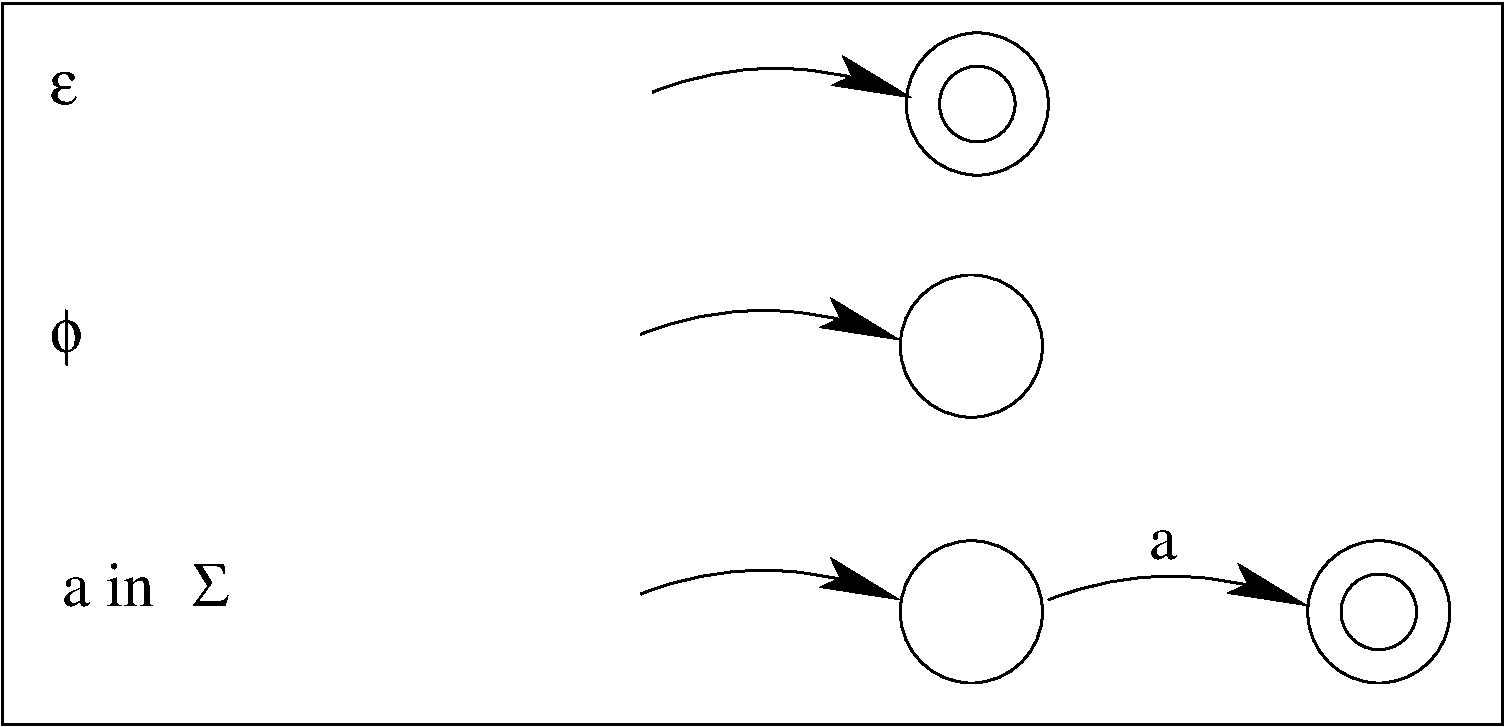
\includegraphics[%
%    width=0.55\linewidth,
%    keepaspectratio]{re2fsa}\end{center}
%  \caption{An NFA for the three base cases\label{re2fsa}}
%  \end{figure}
%  
%  The three {\em recursive} cases are described as follows: let $E_1$
%  and $E_2$ be two regular expressions, then
%  \begin{itemize}
%  \item $NFA_{E_1E_2} = concat(NFA_{E_1},NFA_{E_2})$
%  \item $NFA_{E_1^*} = star(NFA_{E_1})$
%  \item $NFA_{E_1|E_2} = union(NFA_{E_1},NFA_{E_2})$
%  \end{itemize}
%  
%  \begin{theorem}
%  The construction above preserves the language, i.e.
%  
%  ~~~~~~~~~~~~~~~~~~~~~~~~~~~~~~~~~~~~~~~ $L_{NFA_E} = L_E$.
%  \end{theorem}
%  \begin{proof}
%  Prove this yourself - use structural induction.
%  \end{proof}
%  
%  
%  \section{From NFA to Regular Expression}
%  
%  The opposite way is a bit more complicated: we first introduce a new
%  kind of finite automata, the {\em Generalized Non-deterministic Finite
%  Automata} or GNFAs. We will then follow the path:
%  
%  
%  $NFA \rightarrow GNFA \rightarrow GNFA~with~2~states \rightarrow regular~expression$
%  
%  In each of the steps, we must prove that the language stays the same.
%  
%  \begin{definition}[GNFA (informal)]
%  A {\bf GNFA} is a finite state machine with the following
%  modifications and restrictions:
%  \begin{itemize}
%  \item there is exactly one end state and it differs from the start state
%  \item there is exactly one edge from the start state to any other
%  state, but the start state has no incoming edge (except for the start arrow)
%  \item there is exactly one edge from each state to the end state, but
%  the end state has no outgoing edge
%  \item there is exactly one edge between every other two states (in both
%  directions) and an edge from each state to itself
%  \item the edges carry a regular expression as a label
%  \end{itemize}
%  \end{definition}
%  
%  
%  Figure~\ref{gfsa1} shows a GNFA.
%  
%  \begin{figure}[h]
%  \begin{center}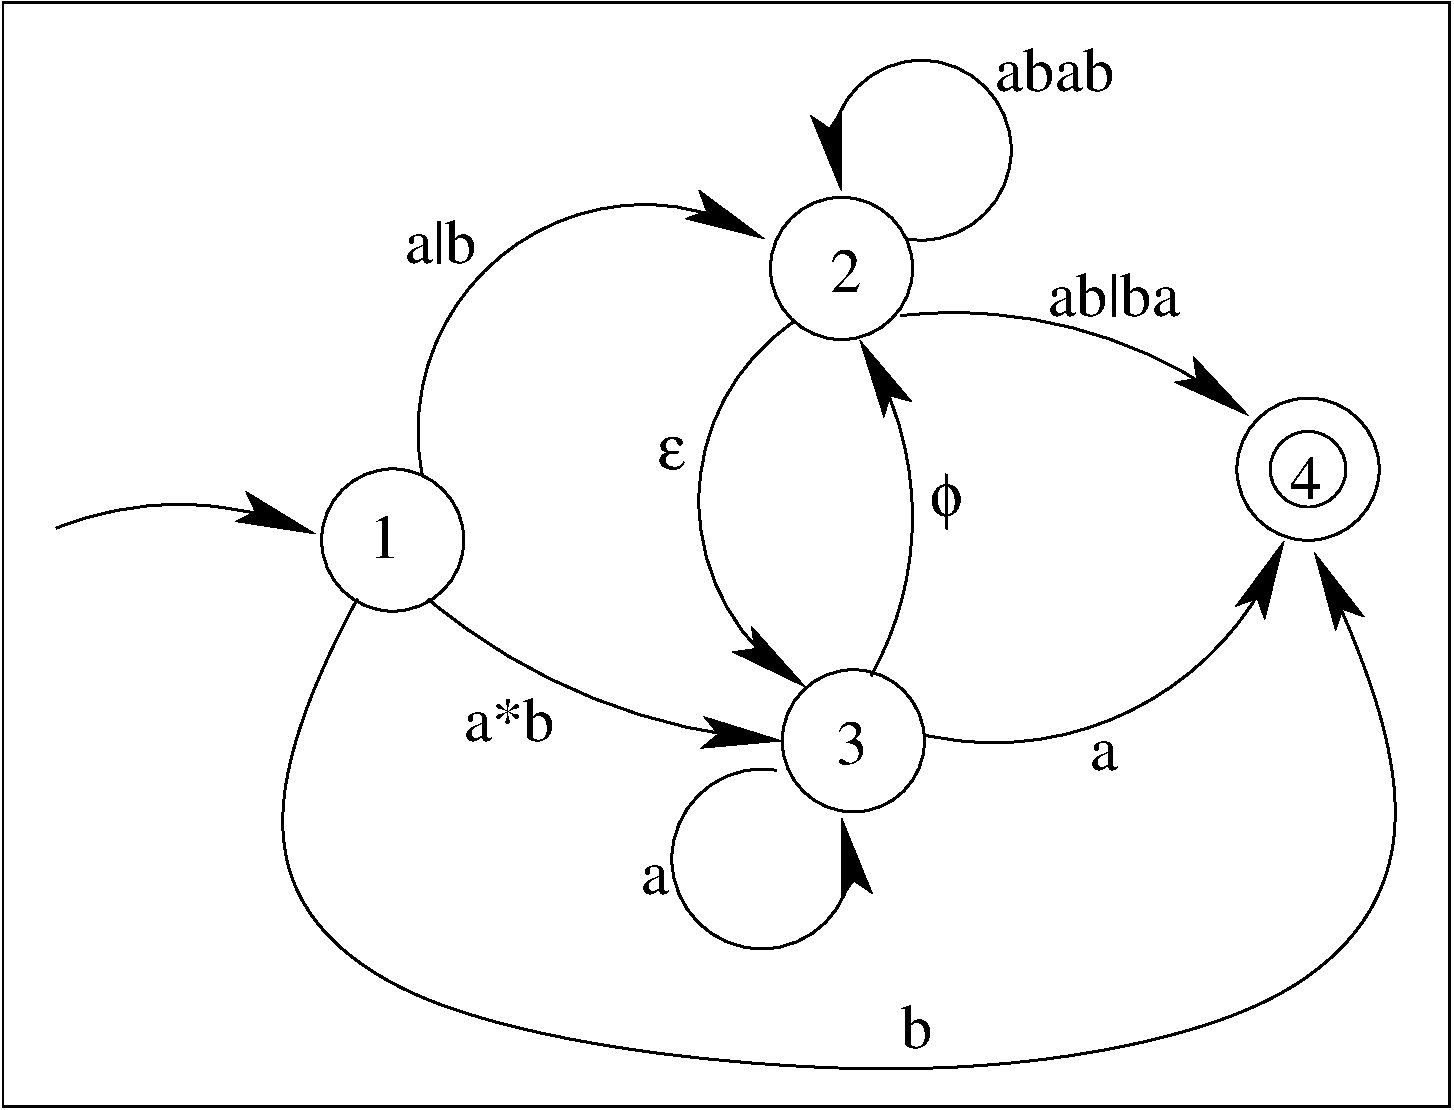
\includegraphics[%
%    width=0.5\linewidth,
%    keepaspectratio]{gfsa1}\end{center}
%  \caption{A GNFA\label{gfsa1}}
%  \end{figure}
%  
%  We use the (graphical representation of the) GNFA as follows:
%  
%  \begin{enumerate}
%  \item you start off with a string $s$ in the start state
%  \item you may now move to any state (the same or another one) by
%  following an edge as long as your string starts with a substring that
%  matches the regular expression on the edge: during the transition, you
%  chop off that substring; if the regular expression equals $\epsilon$,
%  the substring has length zero; if the edge just contains $\phi$, you
%  can't take that edge
%  \item keep making transitions: if you arrive in the end state with an
%  empty string, we say {\em the GNFA has accepted the initial string $s$}
%  \end{enumerate}
%  
%  
%  \paragraph{Selfie:}
%  \begin{itemize}
%  \item[]
%  For the GNFA in Figure~\ref{gfsa1}, find strings accepted by it and
%  strings not accepted by it.
%  \end{itemize}
%  
%  
%  
%  Now is the time to describe an algorithm for constructing a RE from an NFA.
%  
%  \begin{itemize}
%  \item[Step 1:]  {\em Make a GNFA from an NFA}
%  
%  Introduce a new start state and a new unique end state. Draw an
%  $\epsilon$-edge from the new start state to the old start state. and
%  from the old end states to the new end state. Draw all missing edges
%  with label $\phi$. Replace parallel edges into a new edge with as
%  label the union of the labels of the parallel edges.
%  
%  \item[Step 2:]  {\em Reduce the GNFA to a GNFA with two states}
%  
%  Choose any state X different from start and end state: if there is
%  none, go to step 3. Remove X and for each pair of states A and B with
%  an edge
%  % from
%  A to X with $E_1$,
%  %
%  from X to itself with $E_2$,
%  %
%  from X to B with $E_3$,
%  %
%  from A to B with $E_4$,
%  %
%  replace the label on the edge from A to B by
%  $E_4~|~E_1E_2^*E_3$. Finally, remove all edges connected to X.
%  
%  This base step is illustrated in Figure~\ref{redgfsa1}.
%  
%  Repeat step 2.
%  
%  \begin{figure}[h]
%  \begin{center}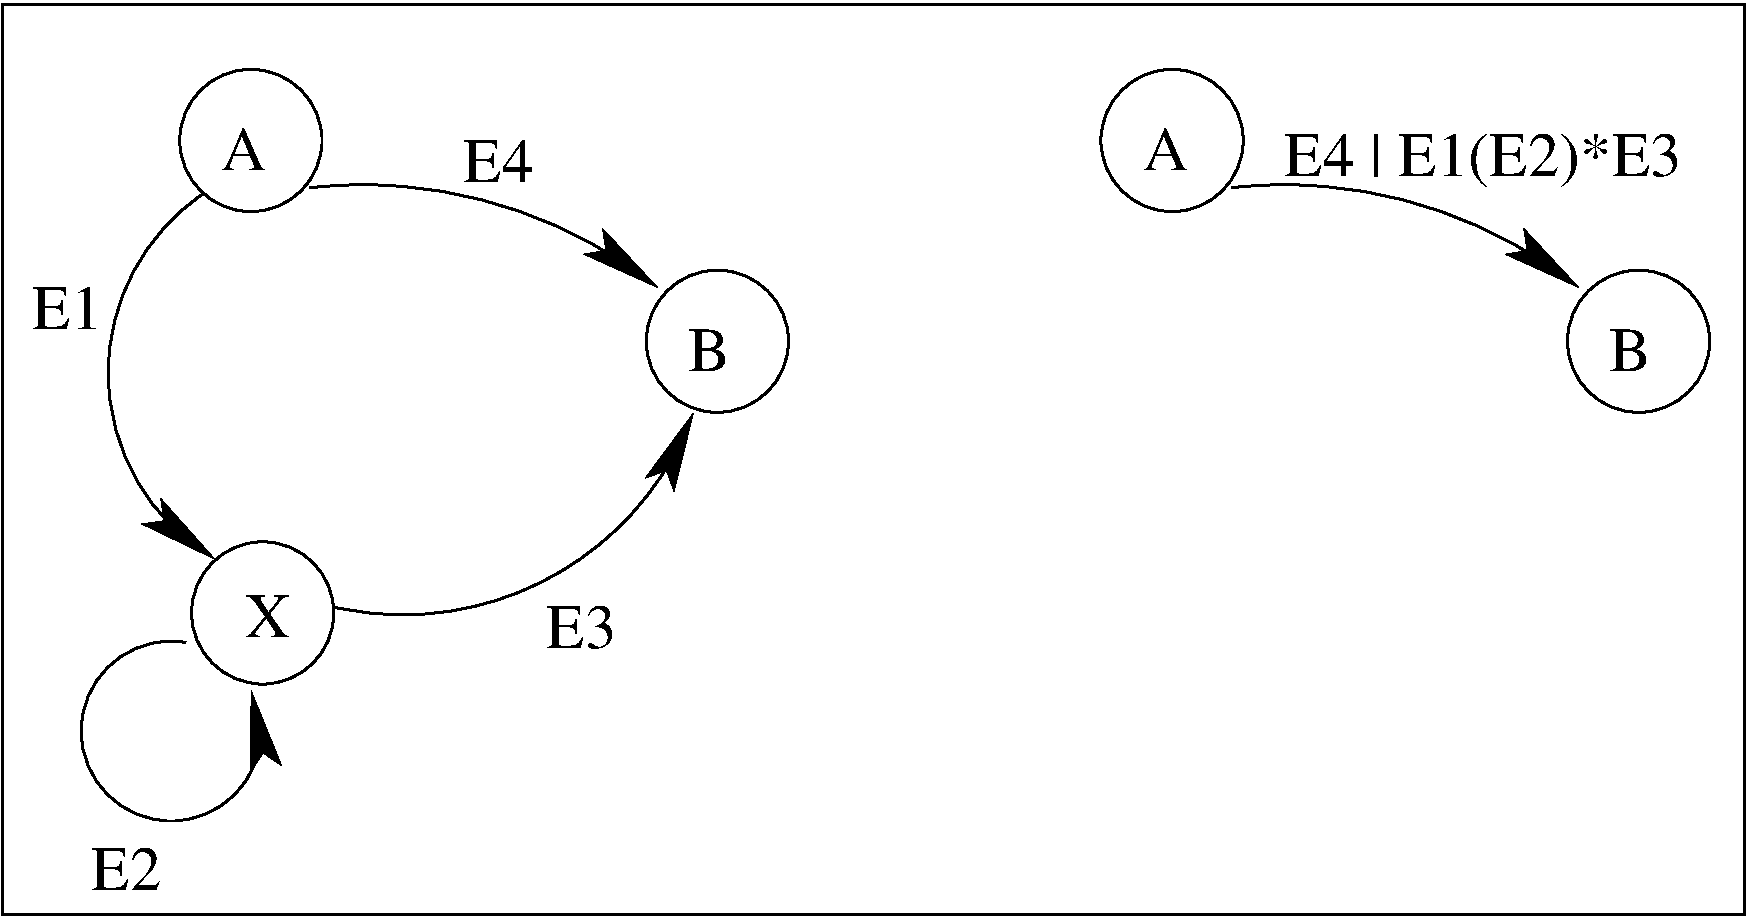
\includegraphics[%
%    width=0.6\linewidth,
%    keepaspectratio]{redgfsa1}\end{center}
%  \caption{Removal of one state from the GNFA \label{redgfsa1}}
%  \end{figure}
%  
%  
%  \item[Step 3:]  {\em Determine the RE}
%  
%  The GNFA has exactly two states: the start and the accepting
%  state. There is only one edge and it has RE as a label.
%  \end{itemize}
%  
%  
%  \paragraph{Example:} Figures~\ref{gfsa2}~and~\ref{gfsa3} illustrate
%  this on the GNFA of Figure~\ref{gfsa1}.
%  
%  
%  \begin{figure}[h]
%  \begin{center}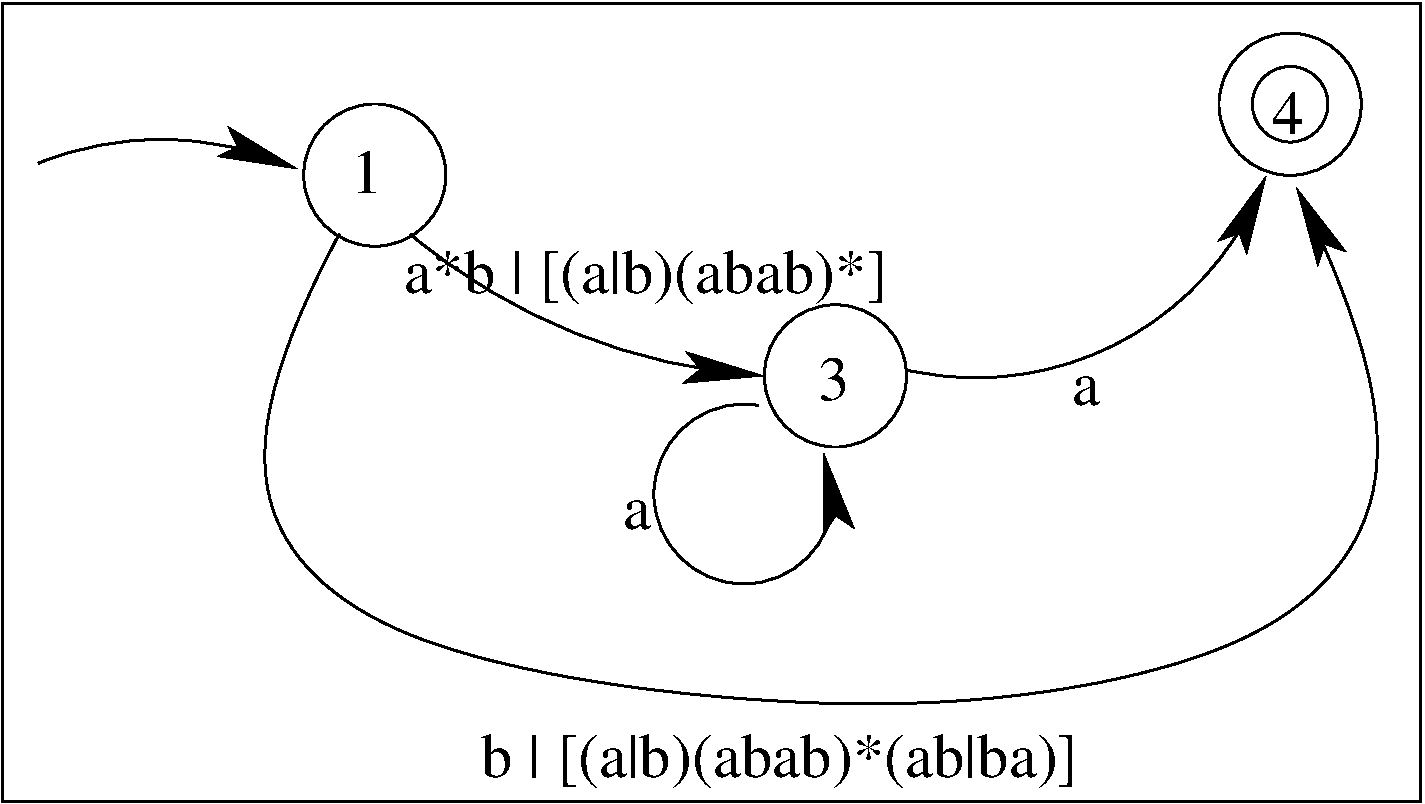
\includegraphics[%
%    width=0.6\linewidth,
%    keepaspectratio]{gfsa2}\end{center}
%  \caption{State 2 was removed \label{gfsa2}}
%  \end{figure}
%  
%  \begin{figure}[h]
%  \begin{center}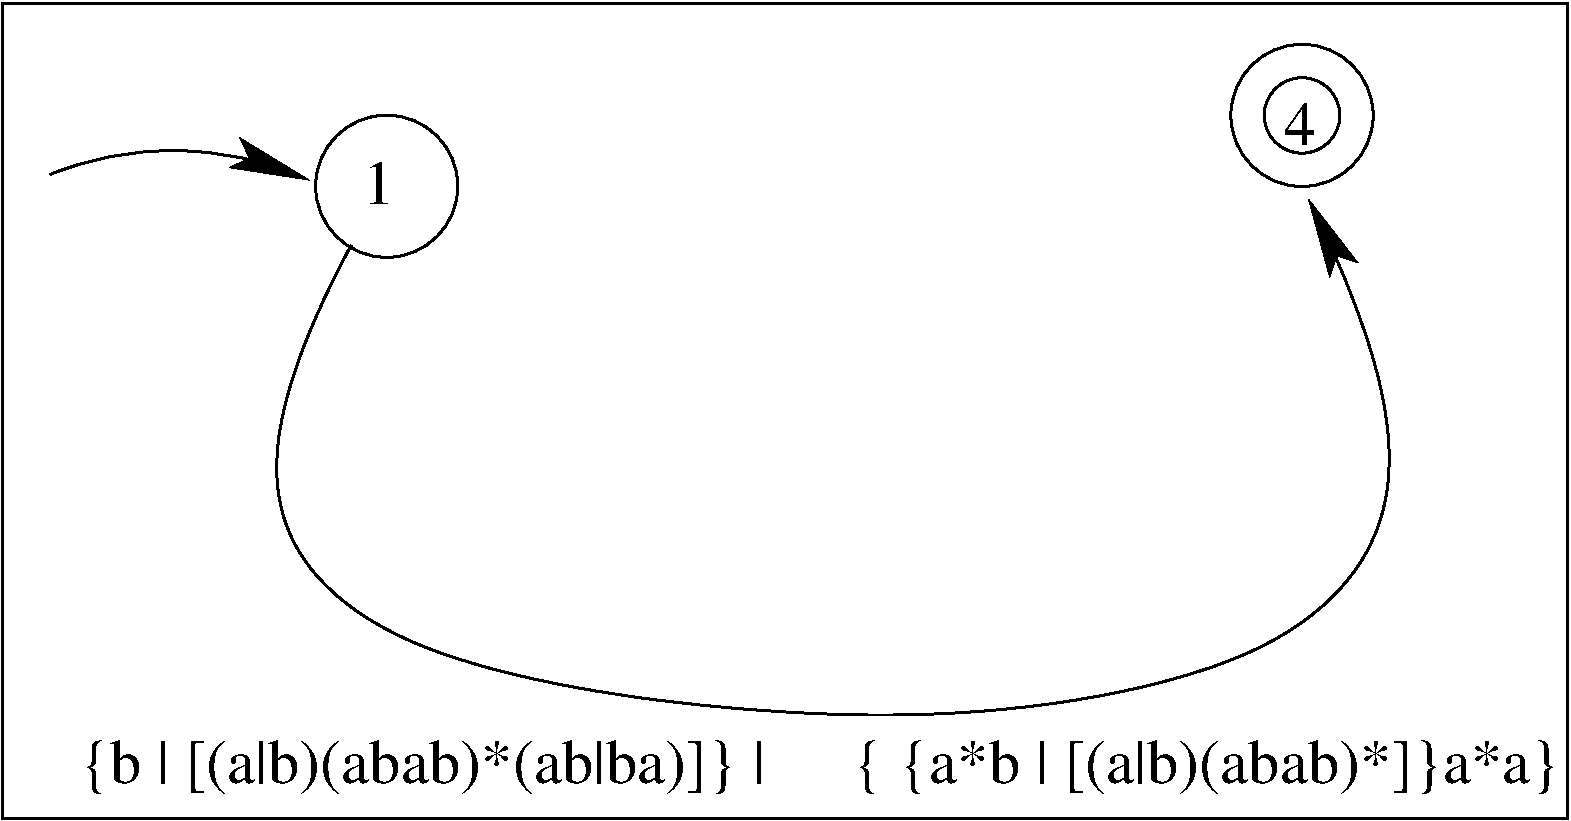
\includegraphics[%
%    width=0.6\linewidth,
%    keepaspectratio]{gfsa3}\end{center}
%  \caption{State 3 was removed \label{gfsa3}}
%  \end{figure}
%  
%  
%  The main thing to prove is that the elimination of X in
%  Step 2 does not change the set of accepted strings. We need to prove
%  two things: (1) if a string $s$ was accepted before the elimination,
%  it is also accepted after elimination; (2) if a string was not accepted
%  before elimination, it is not accepted afterwards.
%  
%  
%  
%  We use the notion of a path through the GNFA that can be followed to
%  accept a string - the related notion for NFAs can be found on page
%  \pageref{defacceptnfa}: write it out for a GNFA. Such an acceptance
%  path is a sequence of states. We denote the GNFA before the reduction
%  by $GNFA_{before}$ and the machine after the reduction by
%  $GNFA_{after}$.
%  
%  \begin{enumerate}
%  \item
%  If $s$ is accepted by $GNFA_{before}$ with a path that does not
%  contain X, then $s$ is accepted by $GNFA_{after}$ with the same path.
%  
%  If the accepting path contains X, then there are states A and B so
%  that for some $n>0$, AX$^n$B is a subsequence in the path. The
%  regular expressions on the edges AX, XX, XB are E1, E2, E3 and
%  therefore, to go from A to B through X {\em costs} a piece of string
%  that matches $E1(E2)^*E3$: that regular expression is part of the
%  regular expression on the edge AB in $GNFA_{after}$, so ...
%  
%  \item
%  If $s$ is accepted by $GNFA_{after}$ then an accepting path cannot
%  contain X. Let AB be a subsequence of the path: on the edges from A to
%  B, part of the regular expression is $E4 | E1(E2)^*E3$: using this
%  while going from A to B, means in $GNFA_{before}$ following the
%  original edge from A to B (with E4), or following AX, XX (as often as
%  needed) and then XB, i.e. $E1(E2)^*E3$. It follows that a string
%  accepted by $GNFA_{after}$ is also accepted by $GNFA_{before}$.
%  
%  \end{enumerate}
%  
%  We also need to justify that the GNFA obtained in step 1 determines
%  the same language as the NFA we started from: please do that.
%  
%  
%  
%  
%  \paragraph{Conclusion:} the two formalisms NFA and RE determine
%  exactly the same class of languages, i.e. the regular languages. Our
%  proofs were constructive and can be transformed into a program in
%  Java, Prolog ... that compute from an RE an NFA, and vice versa.
%  We will go two steps further: we will get rid of the non-determinism
%  in Section~\ref{detfsa}, and we will build the smallest possible
%  machine in Section~\ref{minfsa}.

%  %===============================================================================
%  \section{Deterministic Finite State Machines}\label{detfsa}
%  
%  The definition of a (non-deterministic) finite state machine NFA
%  allows for more than one edge leaving a state with the same symbol,
%  and also with $\epsilon$: both are a source of
%  non-determinism. Indeed, one has the choice to shorten the current
%  string or not, and one has the choice of which state to
%  move to. Implementing this (on the basis of the transition table for
%  instance) is not so difficult, but it is clear that a program that is
%  based on taking steps that might have to backtracked over cannot be
%  optimal. It would be more efficient if there were no $\epsilon$-edges,
%  and if for each symbol in the alphabet, there was only one edge with
%  that label from each state. Such an automaton would be called a
%  deterministic finite state machine, abbreviated as DFA.
%  
%  Formally, we restrict the transition function to the signature
%  %
%  $\delta : Q \times \Sigma \rightarrow Q$, but we allow it to be a
%  partial function. It should be clear that DFAs determine regular
%  languages. 

%  So we are left with the question: is every regular language
%  determined by a DFA? Or, equivalently, we can wonder whether every NFA
%  can be transformed to an equivalent DFA.
%  %
%  We describe this transformation in general.
%  
%  
%  \begin{itemize}
%  \item[{\bf Given:}] an NFA = $(Q_n,\Sigma,\delta_n,q_{sn},F_n)$
%  
%  \item[{\bf To construct:}] a DFA = $(Q_d,\Sigma,\delta_d,q_{sd},F_d)$
%  such that $L_{NFA} = L_{DFA}$
%  
%  \item[{\bf Construction:}]
%  $Q_d = {\cal P}(Q_n)$: one state in the DFA is a set of NFA states
%  
%  $F_d = \{S |S \in Q_d, $S$ \cap F_n \neq \emptyset\}$: an end state in
%  the DFA is any state that contains an NFA end state
%  
%  $\delta_d$ has signature
%  %
%  $\delta_d :  ({\cal P}(Q_n) \times \Sigma) \rightarrow {\cal P}(Q_n)$
%  
%  We first define $er : Q_n \rightarrow {\cal P}(Q_n)$ (er means {\bf
%  e}psilon-{\bf r}eachable):
%  
%  \begin{itemize}
%  \item $er(q)$ is the set of NFA states that can be reached from q
%  using zero, one or more $\epsilon$-edges
%  
%  \item
%  we lift the definition of er to ${\cal P}(Q_n)$ in the usual way: for
%  ${\cal Q} \in {\cal P}(Q_n)$
%  
%  $~~~~~~~~~~~~~~~~~er({\cal Q}) = \cup_{q \in {\cal Q}} er(q)$
%  
%  \item
%  we lift $\delta_n$ in a similar way.
%  \end{itemize}
%  
%  
%  We can now define $\delta_d$ as:
%  \begin{itemize}
%  \item
%  $\delta_d({\cal Q},a) = er(\delta_n({\cal Q},a))$ \footnote{Check the
%  signature!} for ${\cal Q} \in Q_d$
%  
%  \item
%  in words: from a DFA state ${\cal Q}$, you move to the next DFA state
%  by first using the symbol $a$ in each NFA state in ${\cal Q}$ using
%  the NFA transition function, and then following as many
%  $\epsilon$-edges as possible; then take the union of all the NFA
%  states you could reach in this way.
%  
%  \end{itemize}
%  
%  Finally, we define
%  
%  $~~~~~~~~~~~~~~~~q_{sd} = er({q_{sn}})$.
%  
%  
%  \item[{\bf End}]
%  \end{itemize}
%  
%  
%  We use this construction on the NFA of Figure~\ref{fsa2}. This NFA
%  has 3 states, so we might need 8 DFA states.
%  
%  
%  \begin{figure}[h]
%  \begin{center}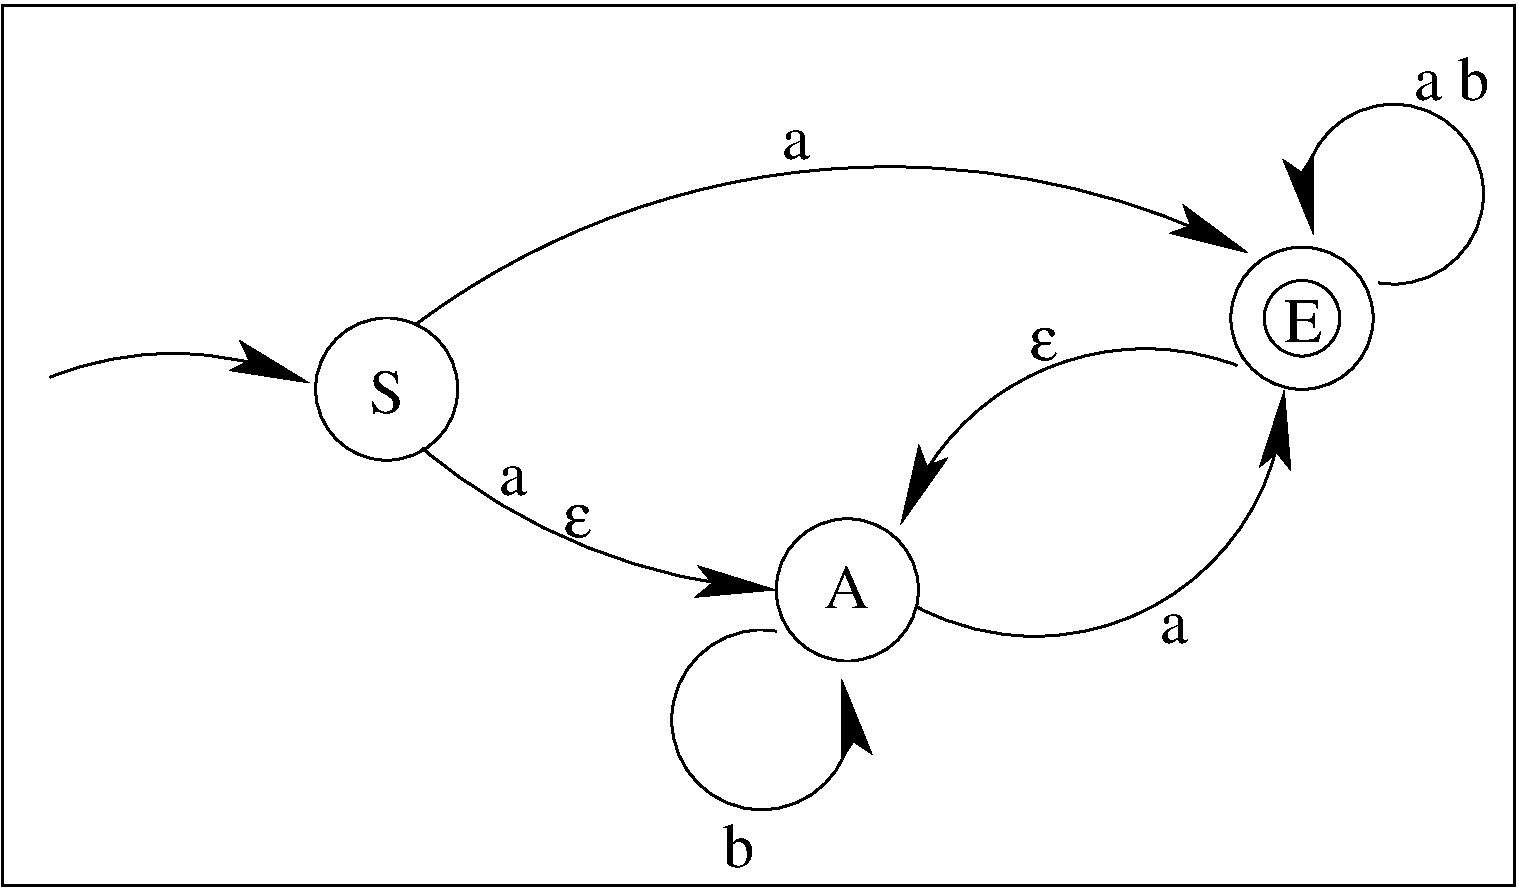
\includegraphics[%
%    width=0.6\linewidth,
%    keepaspectratio]{fsa2}\end{center}
%  \caption{An NFA \label{fsa2}}
%  \end{figure}
%  
%  
%  Table~\ref{charstable} shows the resulting transition table, and er.
%  
%  \begin{table}[ht]
%  \center
%  \begin{tabular}{|r|r|r|r|r|r|}
%  \hline
%  $q \in Q_d$    & $er(q)$  &  $\delta_n(q,a) $ & $\delta_n(q,b) $ & $\delta_d(q,a)$ & $\delta_d(q,b)$ \\ \hline
%  \{\}           & \{\}     &  \{\}             & \{\}             & \{\}            & \{\}            \\
%  \{S\}          & \{S,A\}  &  \{A,E\}          & \{\}             & \{A,E\}         & \{\}            \\
%  \{A\}          & \{A\}    &  \{E\}            & \{A\}            & \{A,E\}         & \{A\}           \\
%  \{E\}          & \{A,E\}  &  \{E\}            & \{E\}            & \{A,E\}         & \{A,E\}         \\
%  \{S,A\}        & \{S,A\}  &  \{A,E\}          & \{A\}            & \{A,E\}         & \{A\}           \\
%  \{S,E\}        & \{S,A,E\}&  \{A,E\}          & \{E\}            & \{A,E\}         & \{A,E\}         \\
%  \{A,E\}        & \{A,E\}  &  \{E\}            & \{A,E\}          & \{A,E\}         & \{A,E\}         \\
%  \{S,A,E\}      & \{S,A,E\}&  \{A,E\}          & \{A,E\}          & \{A,E\}         & \{A,E\}         \\
%  \hline
%  \end{tabular}
%  \caption{The DFA obtained from the NFA in Figure~\ref{fsa2}} \label{charstable}
%  \end{table}
%  
%  
%  Some states are not reachable from the start state $\{S,A\}$. It
%  suffices to represent only the reachable states, as in the graphical
%  representation of the DFA in Figure~\ref{fsa3}.
%  
%  
%  \begin{figure}[h]
%  \begin{center}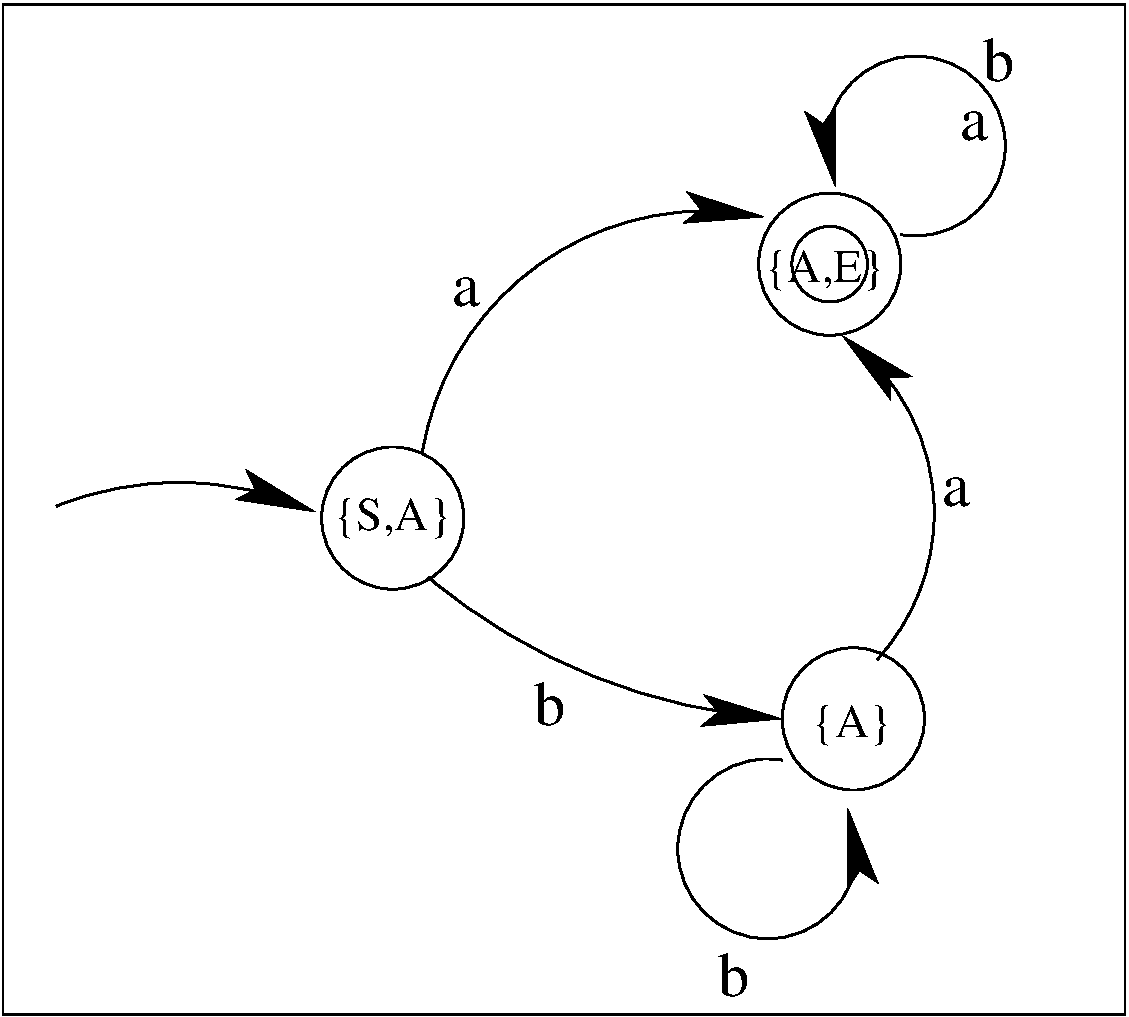
\includegraphics[%
%    width=0.45\linewidth,
%    keepaspectratio]{fsa3}\end{center}
%  \caption{The resulting DFA \label{fsa3}}
%  \end{figure}
%  
%  \paragraph{Selfie:}
%  \begin{itemize}
%  \item[]
%  Which language does the DFA determine? Give an RE for it, or express
%  in words which strings are accepted. Is this the {\em smallest} DFA
%  accepting the same language? What would be a good notion of {\em size}
%  of a DFA?
%  
%  The construction could in the worst case require $2^{\#Q_n}$ DFA
%  states, but the example shows that $Q_d$ does not need to be larger
%  than $Q_n$ if we do not use the unreachable states. Is it possible
%  that the DFA has fewer states than the NFA you start from?
%  \end{itemize}
%  
%  

%  \paragraph{Extending $\delta$ to strings:} the domain of $\delta$ in a
%  DFA is $Q \times \Sigma$. It is useful to extend $\delta$ to a
%  function $\delta^*$ on the domain $Q \times \Sigma^*$ as follows:
%  
%  \begin{itemize}
%  \item $\delta^*(q,\epsilon) = q$
%  \item $\delta^*(q,aw) = \delta^*(\delta(q,a),w)$ if $\delta(q,a)$
%  exists - $a \in \Sigma$ and $w \in \Sigma^*$.
%  \end{itemize}
%  
%  \paragraph{Selfie:}
%  \begin{itemize}
%  \item[]
%  Prove that $\delta^*(q,wa) = \delta(\delta^*(q,w),a)$ for $a \in
%  \Sigma$ and $w \in \Sigma_{\epsilon}^*$
%  \end{itemize}

%===============================================================================
\section{The Minimal DFA}\label{minfsa}

For any regular language L, there exist many DFAs - how many? It is
important to construct small machines: in an application in which a
DFA is needed, you need to represent the transition table in one way
or another, so you might want to keep the number of states low. It is
clear that for a given regular language, there exists a minimal DFA,
i.e. a DFA with the smallest number of states\footnote{Why is that
clear?}. We will construct such a minimal (equivalent) DFA by removing
states from a given DFA. We will prove minimality and even uniqueness.

States that are unreachable from $q_s$ can be removed: that does not
change the language. There can be another way to remove states:
Figure~\ref{mini1} shows at the left a DFA with 5 states.

\begin{figure}[h]
\begin{center}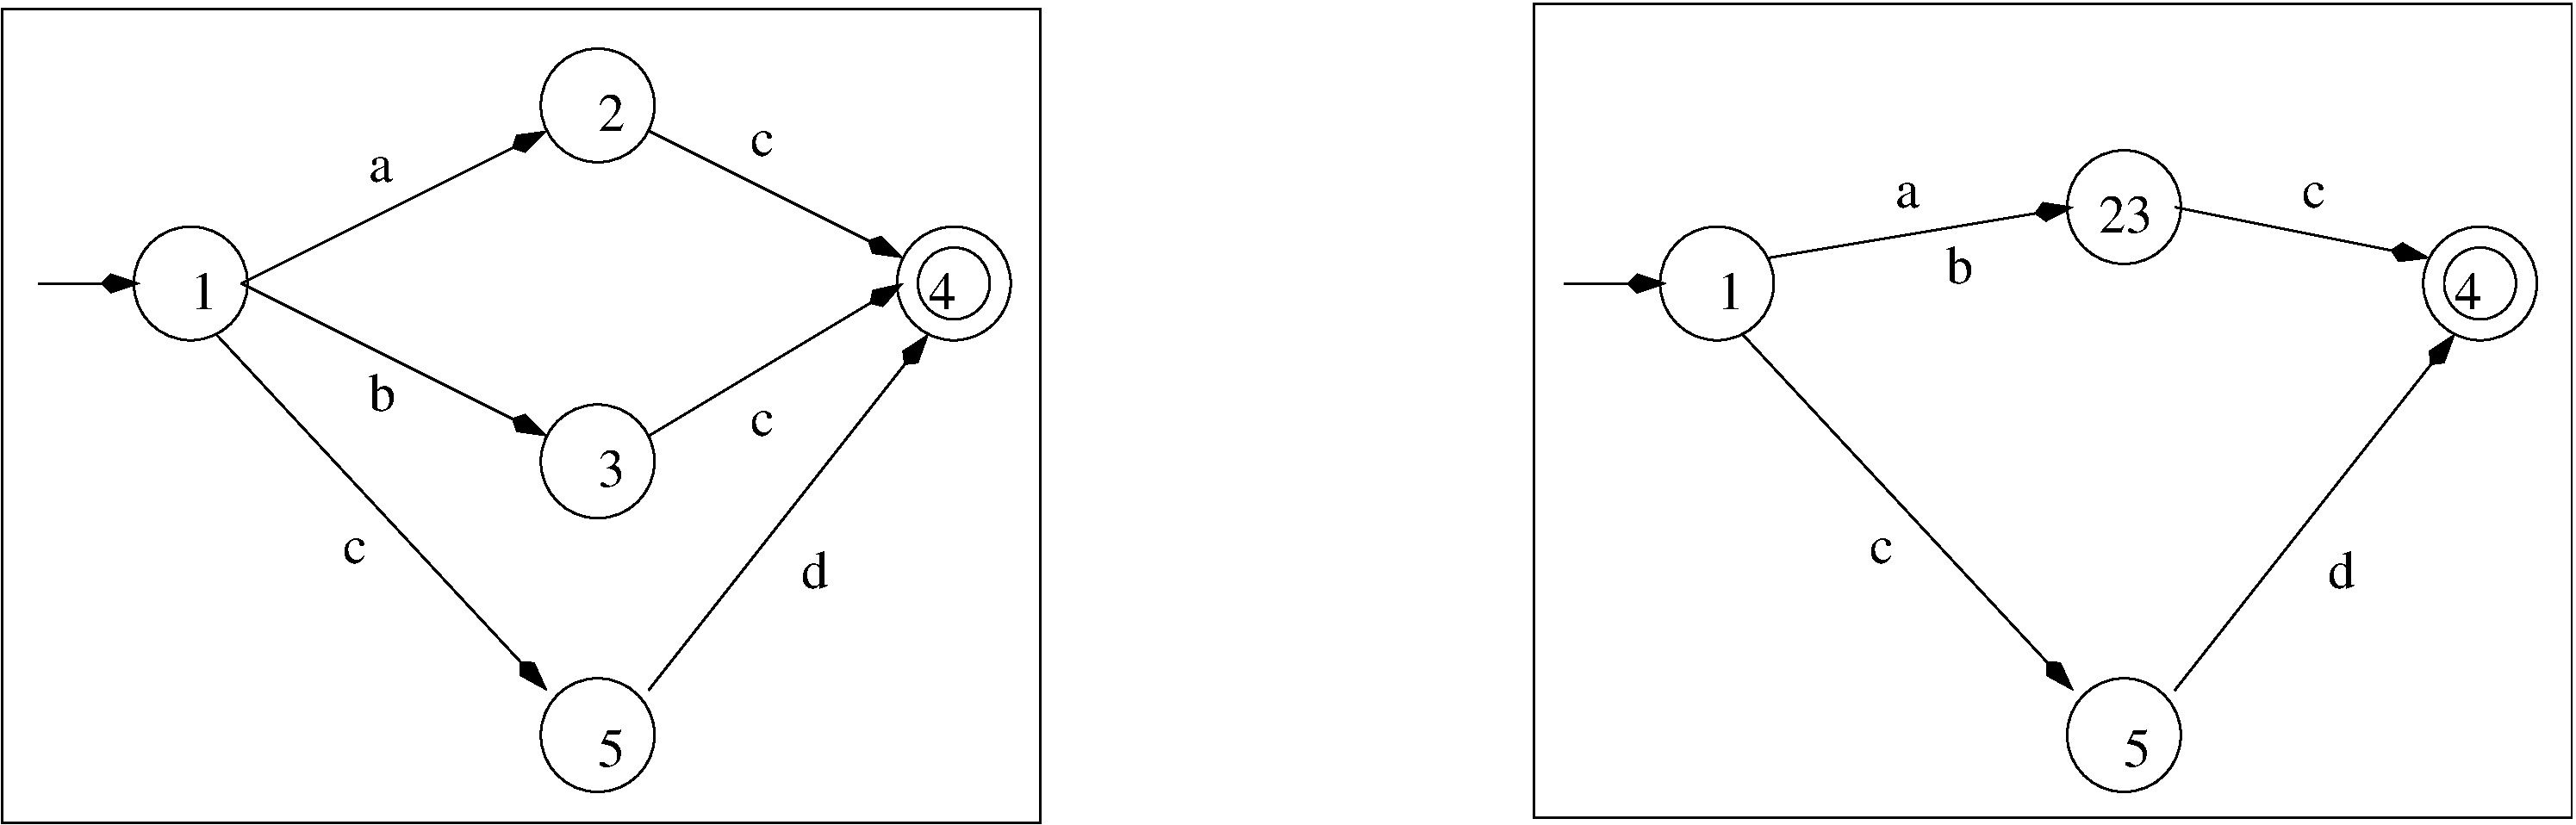
\includegraphics[%
  width=1.0\linewidth,
  keepaspectratio]{mini1}\end{center}
\caption{ On the left a DFA with 2 {\em equivalent} states that were
collapsed on the right.\label{mini1}}
\end{figure}

From states 2 and 3, we see leaving edges with the same label and
arriving in an end state. This shows that the two states are in some
sense indistinguishable: from state 2 and 3, the same strings lead to
F (the set of the final states). On the other hand, states 3 and 5 do not have this property: the
same string can lead to F and not. So, states 3 and 5 are
distinguishable. The minimalisation idea consists in: identify
indistinguishable states and collapse them.

We will assume that $\delta$ is total, i.e. that from each state there
is an outgoing edge for every symbol in the alphabet. A DFA without
that property can be easily transformed to a DFA complying to it:
convince yourself you need at most one extra state.

\begin{definition}[Indistinguishable states] \label{gelijk}
Two states p and q are {\bf indistinguishable} if
$\forall w \in \Sigma^*: \delta^*(p,w) \in F \Longleftrightarrow \delta^*(q,w) \in F$

Two states are {\bf distinguishable} if they are not indistinguishable.
\end{definition}

If $p$ and $q$ are distinguishable, then there exists a word $w$ so that

$~~~~~~~~~~\delta^*(p,w) \in F~~and~~ \delta^*(q,w) \notin F$ or vice versa.


We first informally describe an algorithm to compute sets of
indistinguishable states, and what to do with them.

\begin{itemize}
\item[{\bf Init:}]
a state $p \notin F$ is for sure distinguishable from any state in
F; at this moment, we have not taken a decision about whether any two other states are distinguishable.

\item[{\bf Repeat:}]
take any pair of states $p$ and $q$ about which we have not taken a
decision yet: suppose there is a symbol $a$ so that with $a$ you go
from $p$ and $q$ to distinguishable states; now mark $p$ and $q$ as
distinguishable; repeat until no more such pair exists

\item[{\bf Consolidate:}]
for each pair of states $p$ and $q$ without a decision, decide that
$p$ and $q$ are indistinguishable; indistinguishable is an equivalence
relation, so consider the equivalence classes $Q_i$ within $Q$; these
$Q_i$ will be the states in the minimal DFA; $\delta$ will be shown
later
\end{itemize}

To save on writing, we use $p_a$ as a shorthand for $\delta(p,a)$.


\begin{code} Indistinguishable states \label{gelijketoestanden}
\begin{enumerate}
\item[{\bf Init:}]
Consider the graph $G$ with the states of the DFA as vertices; add an
edge between any two vertices of which exactly one belongs to F and
label these edges with \eps; an edge between $x$ and $y$ with label
$l$ will be denoted by $(x,y,l)$


\item[{\bf Repeat:}]
\underline{If} there exist vertices $p$ and $q$ so that
\begin{itemize}
\item there is no edge between $p$ and $q$
\item $\exists a \in \Sigma: \exists (p_a,q_a,\_) \in G$
\end{itemize}
\underline{then} choose an $a$ with $(p_a,q_a,\_) \in G$
and add $(p,q,a)$ to G; go back to the beginning of Repeat;

\underline{otherwise}: go to Equal;

\item[{\bf Equal:}]
Consider the complement of $G$: each component is a clique; let $Q_i$
be the set of vertices in the $i^{th}$ component; all states in $Q_i$
are indistinguishable; every state in $Q_i$ is distinguishable from
any other state not in $Q_i$

\end{enumerate}

\end{code}
\begin{proof}
The termination of the algorithm is obvious: the maximal number of
edges in $G$ is $N(N-1)/2$ with $N=|Q|$; one such edge is added in
Repeat each time the condition is fulfilled.

We prove that


$~~~~~~~~~~~~~~~(p,q,\_)$ is an edge in $G$ $\Longleftrightarrow$ $p$ and $q$ are distinguishable


$\underline{\Longrightarrow}$: if $(p,q,X)$ is an edge in $G$, then
there are two possibilities: $X = \epsilon$ or $X = a \in \Sigma$; in
the former case, we know that $p$ and $q$ are distinguishable (take
$w = \epsilon$ in the conclusion after the definition of
distinguishable on page \pageref{gelijk}); in the latter case, there
exists an edge of the form $(p_a,q_a,\_)$ in $G$: you can use the
label to arrive (eventually) at the former base case, i.e.
%
$\exists w \in \Sigma^* : \exists (p_w,q_w,\epsilon) \in G$, and we
conclude that $p$ and $q$ distinguishable.

$\underline{\Longleftarrow}$: if $p$ and $q$ are distinguishable, then
there exists a $w$ so that $\delta^*(p,w) \in F~~and~~\delta^*(q,w)
\notin F$ or vice versa; if $w$ is the empty string, the conclusion
holds; if not, then $w$ has a last symbol $z \in \Sigma$ and can be
written as $w = vz$; we then know that $\delta^*(p,w) =
\delta(\delta^*(p,v),z)$ so, between states $\delta^*(p,v)$ and
$\delta^*(q,v)$ there is an edge; we can now get rid of the last
symbol of $v$ etc. until we derive that there is an edge between
$\delta^*(p,\epsilon)$ and $\delta^*(q,\epsilon)$, and we are done.
\end{proof}

We have now constructed the equivalence classes of indistinguishable
states - the $Q_i$ at the end of the algorithm: we are now ready to
define the components of the $DFA_{min}$, starting from a DFA
$(Q,\Sigma,\delta,q_s,F)$ all of whose states are reachable.

$DFA_{min}$ consists of
$(\tilde{Q},\Sigma,\tilde{\delta},\tilde{q_s},\tilde{F})$
with
\begin{itemize}
\item $\tilde{Q} = \{Q_1, Q_2, ...\}$ in which the $Q_i$ are as
  computed by the algorithm

\item
$\tilde{\delta}(Q_i,a) = Q_j$ in which $Q_j$ is obtained by taking any
  $q \in Q_i$ (*) and then taking the $Q_j$ containing $\delta(q,a)$

\item
$\tilde{q_s}$ is the $Q_i$ for which $q_s \in Q_i$

\item
$\tilde{F}$ is the set of $Q_i$ for which $Q_i \cap F \neq \emptyset$
\end{itemize}

Figure~\ref{minim1} illustrates how $G$ evolves for the DFA in
Figure~\ref{mini1}, and the complement of the final graph.
\begin{figure}[h]
\begin{center}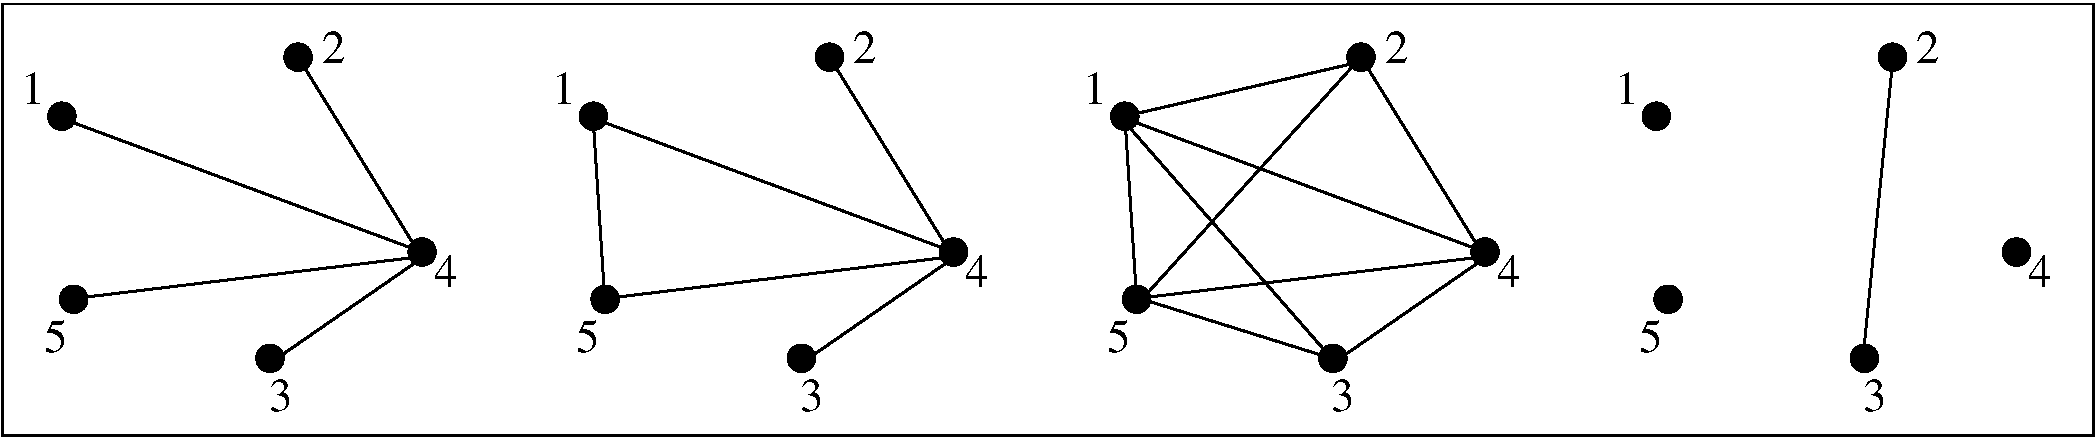
\includegraphics[%
  width=0.9\linewidth,
  keepaspectratio]{minim1}\end{center}
\caption{ 4 steps in the algorithm\label{minim1}}
\end{figure}
\paragraph{Selfie:}
\begin{itemize}
\item[]
In (*) above, really any $q \in Q_i$ can be chosen: prove that this is
indeed true.

Prove that $Q_i \cap F \neq \emptyset$ implies that $Q_i \cap F =
Q_i$, or in words: every element of $Q_i$ belongs to F.

Prove that in $DFA_{min}$ every pair of states is distinguishable.

Finally, prove that $L_{DFA} = L_{DFA_{min}}$

What happens when the algorithm is given a DFA with unreachable states
?
\end{itemize}

\project{collapse NFA naar DFA naar DFA(min) in NFA naar DFA(min)}

We still need to prove that the just constructed $DFA_{min}$ has the
minimum number of states. We prove a slightly stronger theorem:

\begin{theorem}
If $DFA_1 = (Q_1,\Sigma,\delta_1,q_s,F_1)$ is a machine in which all of the
states are reachable, and with every pair of states distinguishable,
then there is no equivalent DFA with strictly fewer states.
\end{theorem}
\begin{proof}
Let $DFA_1$ have states $\{q_s,q_1,...,q_n\}$: $q_s$ is the starting
state. Assume that
%
$DFA_2 = (Q_2,\Sigma,\delta_2,p_s,F_2)$ is a DFA with strictly fewer
states $\{p_s,p_1,...,p_m\}$ than $DFA_1$.

Since in $DFA_1$ every state is reachable, there exist strings $s_i,
i=1..n$ such that
%
$\delta_1^*(q_s,s_i) = q_i$.


Since $DFA_2$ has less states, there must exist $i \neq j$ so that

$~~~~~~~~~\delta_2^*(p_s,s_i) = \delta_2^*(p_s,s_j)$.


Since $q_i$ and $q_j$ are distinguishable, there exists a string $v$
so that


$~~~~~~~~~\delta_1^*(q_i,v) \in F_1 \wedge \delta_1^*(q_j,v) \notin F_1$ or vice versa.

Consequently,
%
$\delta_1^*(q_s,s_iv) \in F_1 \wedge \delta_1^*(q_s,s_jv) \notin F_1$
or vice versa, meaning that $DFA_1$ accepts $s_iv$ or $s_jv$ but not
both.


On the other hand, in $DFA_2$ we have
$\delta_2^*(p_s,s_iv) = \delta_2^*(\delta_2^*(p_s,s_i),v) =
\delta_2^*(\delta_2^*(p_s,s_j),v) = \delta_2^*(p_s,s_jv)$
which means that $DFA_2$ accepts both string $s_iv$ and $s_jv$,
or rejects both.

It follows that $DFA_1$ and $DFA_2$ are not equivalent.
\end{proof}

All states of the constructed $DFA_{min}$ are reachable, and they are
pairwise distinguishable, so our $DFA_{min}$ has the minimum possible
number of states.



Two DFAs can only be really the same if their states are the same, or
otherwise said, if their states have the same name. Also, their
$\delta$, final states and start state must be the same. Still, two
DFAs (on the same alphabet) can be similar except for the names of the
states. We express that by the notion of a DFA isomorphism.

\begin{definition}[Isomorphic DFAs]
$DFA_1 = (Q_1,\Sigma,\delta_1,q_{s1},F_1)$ is {\bf isomorphic} to
  $DFA_2 = (Q_2,\Sigma,q_{s2},\delta_2,F_2)$ if there exists a
  bijection
%
$b: Q_1 \rightarrow Q_2$ so that
\begin{itemize}
\item $b(F_1) = F_2$
\item $b(q_{s1}) = q_{s2}$
\item $b(\delta_1(q,a)) = \delta_2(b(q),a)$ (see Figure~\ref{diagram1})
\end{itemize}
\end{definition}

\begin{figure}[h]
\begin{center}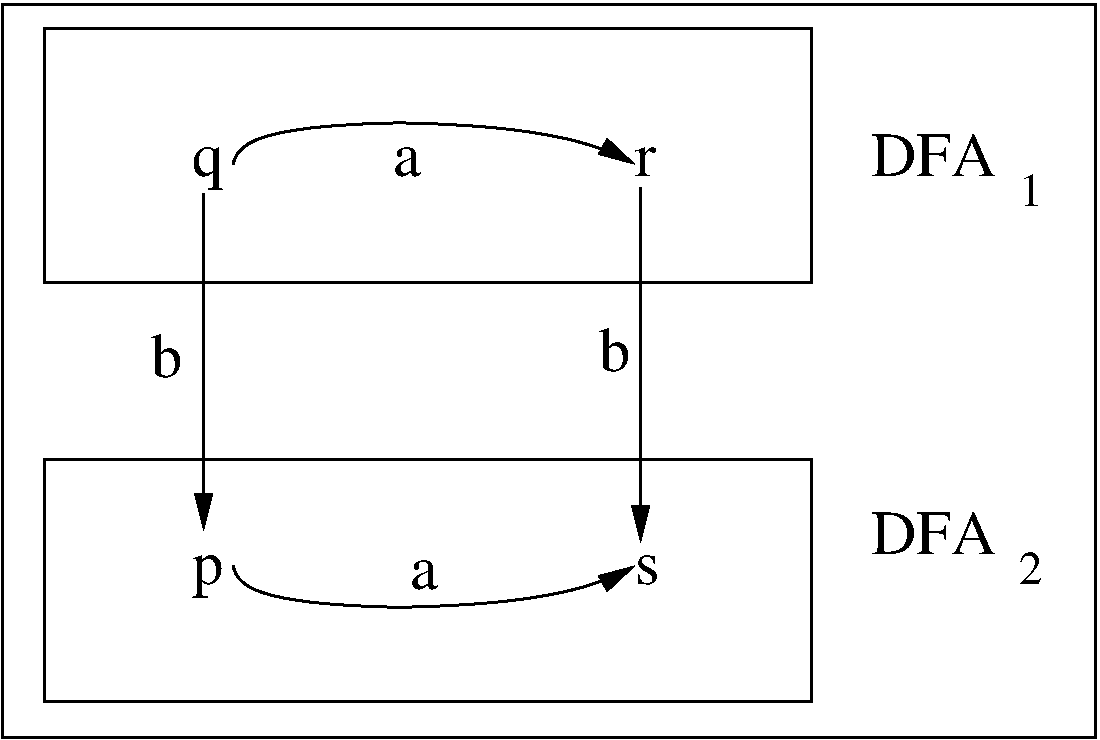
\includegraphics[%
  width=0.4\linewidth,
  keepaspectratio]{diagram1}\end{center}
\caption{Commutative diagram for $b$ and $\delta_i$\label{diagram1}}
\end{figure}


You should be able to prove that two isomorphic DFAs are equivalent
(but not necessarily the other way around).



We can now prove that the minimal DFA is unique up to isomorphism -
give it a try! You can start from the observation that two equivalent
DFAs whose states are reachable and distinguishable must have the same
number of states ...


%% \subsection{De complexiteit van minimizatie en equivalentie}
%%
%% Een DFA minimalizeren kan in polynoomtijd, maar het minimalizeren
%% van NFAs is NP-hard. Het testen van de equivalentie van regular
%% expressions is zelfs PSPACE-hard. Dat kan je intu\"itief argumenteren
%% door te wijzen op het feit dat de conversie van NFAs naar DFAs het
%% aantal toestanden exponentieel kan doen toenemen.


\section{The Pumping Lemma for Regular Languages}

In this section, we get acquainted with a method to prove that a given
language is not regular. Before doing that, here are two arguments why
there exist non-regular languages: it is up to you to make those
arguments more concrete, if not now, certainly later:
\begin{enumerate}

\item
the number of DFAs (over a fixed alphabet) is countably infinite; the
number of languages is uncountably infinite ...

\item
the complexity of deciding whether a string $s$ belongs to a given
regular language, is linear in the size of $s$; since there are
decision problems with a higher complexity ...

\end{enumerate}


Suppose we have an infinite regular language $L$. $L$ has a DFA
deciding it. This DFA has $N = \#Q$ states. Consider a string $s \in
L$ so that $|s| \geq N$, and follow the acceptance path through the DFA
with that string until you reach F. Since the string is longer than
the number of states, at least one state occurs twice in that path:
the path contains a cycle. That cycle {\em consumes} a part $y$ of the
string $s$, and $s = xyz$ where $x$, $y$ and $z$. Convince yourself
that with the string $xyyz$ you could also reach F, and more generally
with $xy^iz$ for any $i \geq 0$.

More formally

\begin{theorem}[The pumping lemma for regular languages]
For every regular language $L$, there exists a pumping length $d$,
so that
%
for all $s \in L$ with $|s| \geq d$, there exists a division of $s$ in
three parts $s = xyz$ and
\begin{enumerate}
\item
$\forall i \ge 0: xy^iz \in L$


\item
$|y| > 0$


\item
$|xy| \leq d$
\end{enumerate}
\end{theorem}
\begin{proof}
Take any DFA that determines $L$. Take $d = \#Q$.

Let $s \in L$ and $s = a_1a_2...a_n$ with $n \geq d$.
Consider the sequence of states along the accepting path of $s$:
$(q_s=q_1,q_2,...,q_{n+1})$: its length is strictly larger than $d$,
so in the first $d$ elements of this sequence, there must be a
repeated state. Assume that $q_i$ equals $q_j$, with $i < j \leq d$,
then define $x = a_1a_2...a_{i}$, $y = a_{i+1}...a_j$, and $z$ the
rest of the string. All statements now follow easily.
\end{proof}

Figure~\ref{pomp1} illustrates the division of $s$ as $xyz$.
\begin{figure}[h]
\begin{center}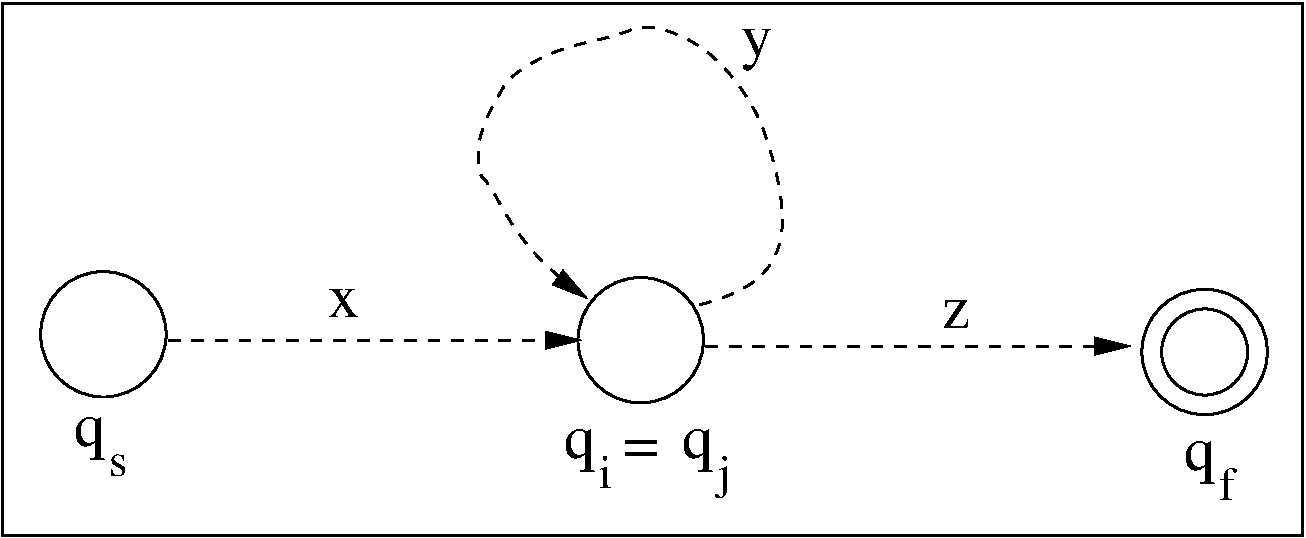
\includegraphics[%
  width=0.5\linewidth,
  keepaspectratio]{pomp1}\end{center}
\caption{$s = xyz$ \label{pomp1}}
\end{figure}


\subsection{Using the pumping lemma}

First convince yourself that you cannot use the pumping lemma for
proving that a given language is regular. In fact, there are languages
whose strings can be pumped, but which are not regular.

The classical example for applying the pumping lemma is the language
$L = \{a^nb^n|n \in \N\}$ over the alphabet $\{a,b\}$.

Suppose that language has a pumping length $d$; consider the string
$s = a^db^d$. Take any division of $s = xyz$ with $|y| > 0$. There are
now three possibilities:

\begin{itemize}
\item y contains only a's: then xyyz contains more a's than b's and
  does not belong to $L$
\item y is of the form $a^ib^j$ with $i \neq 0, j \neq 0$: then
xyyz has some a's and b's in the wrong order, so that string is not in
$L$
\item y contains only b's: then xyyz contains more b's than a's and
  does not belong to $L$
\end{itemize}

As a consequence, $L$ is not regular.

We have not used point 3 in the theorem. If we do, the proof becomes
shorter and easier. Suppose that language has a pumping length $d$;
consider the string $s = a^db^d$. Take any division of $s = xyz$ with
$|y| > 0$ and $|xy| \leq d$. Now $y$ contains only a's and ...



\paragraph{Note:} Using the pumping lemma to prove that $L$ is not
in RegLan, needs the following:
\begin{itemize}
\item for any number $d$ chosen as pumping length
\item there exists a string $s \in L$ longer than $d$
\item for which {\bf every} division $xyz$ prevents pumping
  (i.e. there is an $i$ for which $xy^iz$ is not in $L$)
\end{itemize}

Especially the latter is important - here is an example of how not to
use the lemma. Take as $L$ the language generated by the regular
expression $ab^*c$.  We prove (wrongly !) that $L$ is not regular:
take any pumping length $d > 0$ and take the string $ab^dc$. Divide that
string as $abc = xyz$ with $x = \epsilon$, $y = a$ and $z =
bc$. Clearly, $xyyz$ is not in $L$ so $L$ is not regular ... or is it?

\paragraph{Selfie:}
\begin{itemize}
\item[]
Which error was made above?

Define some languages and try to use the pumping lemma to prove they
are not regular.

Is the language of the regular expressions (over a fixed alphabet)
regular itself?

Prove: every regular language has a minimal pumping length. Is it
related to the minimal DFA for that language?
\end{itemize}

% \newpage
%===============================================================================
\section{DFA Product}

Given are two DFAs $A_1$ and $A_2$ with $A_1 = (Q_i,\Sigma,\delta_i,q_{si},F_i)$ for
i=1,2. These DFAs define two languages $L_{A_1}$ and $L_{A_2}$. How do we obtain
a DFA $B = (Q_B,\Sigma,\delta_B,q_{sB},F_B)$ whose language $L_B = L_{A_1}
\odot L_{A_2}$ with $\odot$ some binary operator on sets like $\cup$,
$\cap$, $\setminus$, $\ominus$, \ldots

We can bring $L_B = L_{A_1} \odot L_{A_2}$ down from the set level to the
string level by mapping the binary set operator $\odot$ to an appropriate binary
boolean operator $\circledast$. For instance, $w \in (L_{A_1} \cup L_{A_2})$
iff $(w \in L_{A_1}) \vee (w \in L_{A_2})$. Similarly, we have to map $\cap$ to $\wedge$,
$\setminus$ to $>$, and $\ominus$ to $\oplus$ (exclusive or). More abstractly, 
we can say that $w \in (L_{A_1} \odot L_{A_2})$ iff $(w \in L_{A_1}) \circledast (w \in L_{A_2})$

This transformation of the problem is useful because we have translated the
membership test of the combined language into a membership test on the given
languages. We don't know how to do the former, but we have automata available
for the latter. Indeed $w$ belongs to $L_(A_i)$ iff $\delta_i(q_{si},w) \in
F_i$. Hence, to determine $w \in L_B$ we can compute $(\delta_1(q_{s1},w) \in
F_1) \circledast (\delta_2(q_{s2},w) \in F_2)$.

The string $s$ is of course of the general form $s = a_1 \cdots a_n$ with all $a_j \in
\Sigma$ and $n \geq 0$. This means that the membership tests on the two automata proceed
through $n + 1$ states of the two automata:
\begin{equation*}
\begin{array}{ccccccc}
q_{s1} & \stackrel{a_1}{\longrightarrow} & q_{11} & \stackrel{a_2}{\longrightarrow} & \cdots & \stackrel{a_n}{\longrightarrow} & q_{n1} \\
q_{s2} & \stackrel{a_1}{\longrightarrow} & q_{12} & \stackrel{a_2}{\longrightarrow} & \cdots & \stackrel{a_n}{\longrightarrow} & q_{n2}
\end{array}
\end{equation*}
where $q_{j1} \in Q_1$ and $q_{j2} \in Q_2$. Observe that these two transition
sequences operate in lockstep: they take the same number of steps, and each
step with the same symbol. Hence, we can actually merge the two transitions 
on different state spaces into one transition on the product of the state spaces:
\begin{equation*}
\begin{array}{ccccccc}
(q_{s1}, q_{s2}) & \stackrel{a_1}{\longrightarrow} & (q_{11}, q_{12}) & \stackrel{a_2}{\longrightarrow} & \cdots & \stackrel{a_n}{\longrightarrow} & (q_{n1}, q_{n2}) 
\end{array}
\end{equation*}
This of course a regular transition sequence in the automaton $B$ that
is defined as:
\begin{itemize}
\item $Q_B = Q_1 \times Q_2$
\item $\delta_B((p, q),x) = (\delta_1(p,x), \delta_2(q,x))$
\item $q_s = (q_{s1}, q_{s2})$
\end{itemize}
Finally, we have to define $F_B \subseteq Q_1 \times Q_2$ in such a way 
that $(q_{n1},q_{n2}) \in F_B$ iff $(q_{n1} \in F_1) \circledast (q_{n1} \in F_1)$.

This depends on the choice of $\circledast$ and thus the underlying choice of $\odot$.
\begin{itemize}
\item If $\odot \equiv \cap$, $\circledast \equiv \wedge$, then $F_B = F_1
      \times F_2$. Then $B$ defines the intersection of the two given languages.
\item If $\odot \equiv \cup$, $\circledast \equiv \vee$, 
      then $F_B = (F_1 \times Q_2) \cup (Q_1 \times F_2)$. 
      Then $B$ defines the union of the two given languages.
\item If $\odot \equiv \setminus$, $\circledast \equiv >$, 
      then $F_B = F_1 \times \overline{F}_2$.
      Then $B$ defines the difference of the two given languages.
\item If $\odot \equiv \ominus$, $\circledast \equiv \oplus$, 
      then $F_B = (F_1 \times \overline{F}_2) \cup (\overline{F}_1 \times F_2)$.
      Then $B$ defines the symmetric difference of the two given languages.
\end{itemize}
Here $\overline{F}_i$ is the complement of $F_i$, which can be obtained as
$Q_i\setminus F_i$.

The above constructions show that the union, the intersection, and the
(symmetric) difference of two regular languages are also regular. It
follows that also the complement is regular, since
%
$\overline{L} = \Sigma^* \setminus L$.

\paragraph{Selfie:}
\begin{itemize}
\item[]
Find a simpler construction of the complement of a given DFA.

% Now use that same construction on an NFA; do you get what you wanted?
% Why (not)?
\end{itemize}

% \newpage
%===============================================================================
\section{Discussion}

\subsection{Regular Expressions and Lexical Analysis}

It is often easy to use a regular expression to specify which {\em
  input} is allowed within a certain context. For instance


~~~~~~~~~~~~$20(0|1|2|3|4|5|6|7|8|9)(0|1|2|3|4|5|6|7|8|9)$

indicates that any year in this century may be input.

Also, the lexical tokens of a programming language are often specified
by REs. The following could be a small part of the Java lexicon:
$(a|b|c)(a|b|c|0|1|2)^*~|~(-|\epsilon)(1|2)(0|1|2)^*$ which describes
identifiers that start with the letter a,b or c, after which are
followed by any number of those three letters and digits (only 0,1,2),
and integers that can start with a minus sign.

Such a specification becomes clumsy without the use of
abbreviations. So one typically specifies a lexicon as follows:


~~~~~~~~~~~~$PosDigit \leftarrow 1~|~2~|~3~|~4~|~5~|~6~|~7~|~8~|~9$

~~~~~~~~~~~~$Digit \leftarrow PosDigit~|~0$


~~~~~~~~~~~~$ThisCentury \leftarrow 20DigitDigit$

and the general form of an integers as $(+|-|\epsilon)PosDigit~Digit^*~|~0$

or the general form of a bank account number:


~~~~~~~~~~~~$BANKNR \leftarrow Digit^3(-~|~\epsilon)Digit^7(-~|~\epsilon)Digit^2$

As for the Java lexicon:


\begin{itemize}
\item[]
$JavaProgr \leftarrow (Id|Int|Float|Op|Delimiter)^*$

$Id \leftarrow Letter~(Letter|Digit)^*$

$Digit \leftarrow PosDigit~|~0$

$PosDigit \leftarrow 1~|~2~|~3~|~4~|~5~|~6~|~7~|~8~|~9$

$Sign \leftarrow (+|-|\epsilon)$

$Unsigned \leftarrow PosDigit~Digit^*$

$Int \leftarrow Sign~Unsigned$

$Float \leftarrow Int~.~Unsigned$

...
\end{itemize}

\label{flexlabel}
The description of a lexicon can be used to automatically construct a
{\em lexer} for Java, i.e. a program that takes a Java program as input,
and breaks it up into lexical units. You are at this moment actually
capable of doing that: you got all the theory to make a good lexer!

There exist tools that do that for you: e.g. flex
\verb|http://flex.sourceforge.net/|) generates C-code: the C-code
implements the DFAs (and necessary glue-code, and even error
handling). jflex (\verb|http://www.jflex.de/|) is based on the same principle and generates Java code. flex and jflex are both lexical
analysis generators.

\paragraph{Selfie:}
\begin{itemize}
\item[]
Read more about (j)flex.

Write a program (pick your language) that takes as input a regular
expression E, and produces a Prolog program with a predicate lex/1: a
query like ?- lex({\em string}). should succeed if and only if {\em
  string} is in $L_E$. You can represent a string like ``abc'' as the
list $[a,b,c]$. An RE like $a^*b~|~c$ can be represented as the term
$or([star(a),b],[c])$ (but you are welcome to try another one).
\end{itemize}

\paragraph{The description} above of a $JavaProgr$, is actually a
BNF-grammar: it is in {\em Backus-Nauer form}: this form is actually
meant for context free languages. BNF can also be used for regular
languages, because they are context free as well: see
Section~\ref{contextvrijelanguages}.

%  \subsection{Variants of Finite State Automata}
%  
%  \subsection{The transducer}
%  
%  \project{minimisatie van transducer}
%  
%  A transducer transforms an input string into an output string: we
%  adapt the definition of a DFA, so that it can produce output. One
%  figure is almost worth a definition.
%  
%  \begin{figure}[h]
%  \begin{center}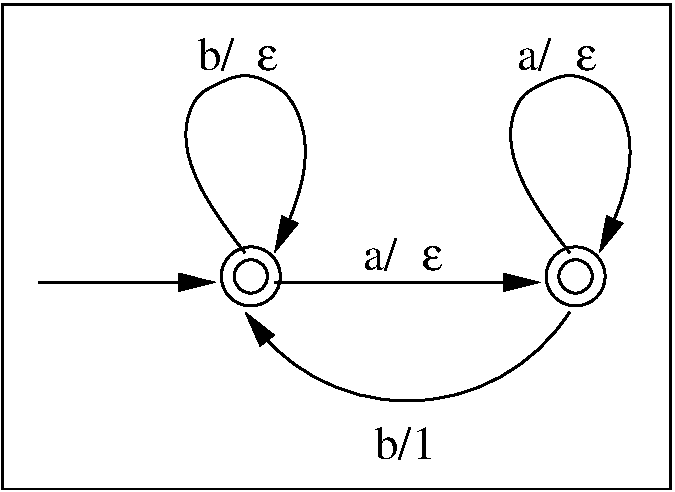
\includegraphics[%
%    width=0.35\linewidth,
%    keepaspectratio]{trans1}\end{center}
%  \caption{A simple transducer \label{trans1}}
%  \end{figure}
%  
%  The labels on the arcs have the form $a/x$: $a$ belongs to the input
%  alphabet, $x$ to the output alphabet. $x$ can also be the empty
%  string. The $a$ is used for finding a path in the transducer as if it
%  were a DFA. The $x$ is output when the edge is used.
%  The above transducer accepts every string and outputs a 1 for every
%  $b$ that follows an $a$.
%  
%  
%  
%  \subsection{A DFA that can check an addition}
%  
%  Since a DFA can only be used for deciding whether a string belongs to
%  a language, we define the language of correct additions. If that
%  language is regular, we should be able to build a DFA for it. Let's do
%  it as follows: $\Sigma = \{0,1\}$. The two numbers we want to add and
%  the result are represented in binary, in reverse order. We also add
%  leading zeros so that all three numbers have the same length. As an
%  example: adding 3 to 13 with result 16 gives us the strings
%  11000 10110 and 00001. We merge them systematically, i.e. we make
%  groups of 3 bits occurring in the i-th place, and write those groups
%  in a sequence. This way we obtain
%  
%  $~~~~~~~~~~~~~~$110 100 010 010 001
%  
%  (the spaces are there only for showing the groups of three)
%  As a result, the string 110100010010001 represents the correct
%  addition 3+13=16. A DFA for this language is in Figure~\ref{telop}.
%  
%  
%  \begin{figure}[h]
%  \begin{center}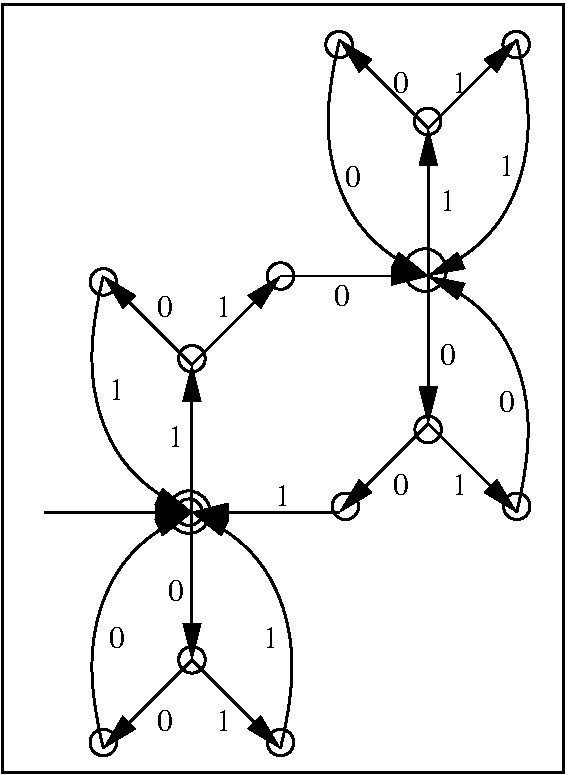
\includegraphics[%
%    width=0.25\linewidth,
%    keepaspectratio]{telop}\end{center}
%  \caption{An addition checker \label{telop}}
%  \end{figure}
%  
%  
%  \subsection{Adding by using a transducer}
%  
%  Addition is: given two numbers as input, output their sum. This is
%  possible with a transducer: use the same representation as before for
%  the two numbers to be added, and merge them in the same way. So 3+13
%  is represented by the string 1110010100. Figure~\ref{telop2} shows two
%  addition transducers that are derived from the checker.
%  
%  \begin{figure}[h]
%  \begin{center}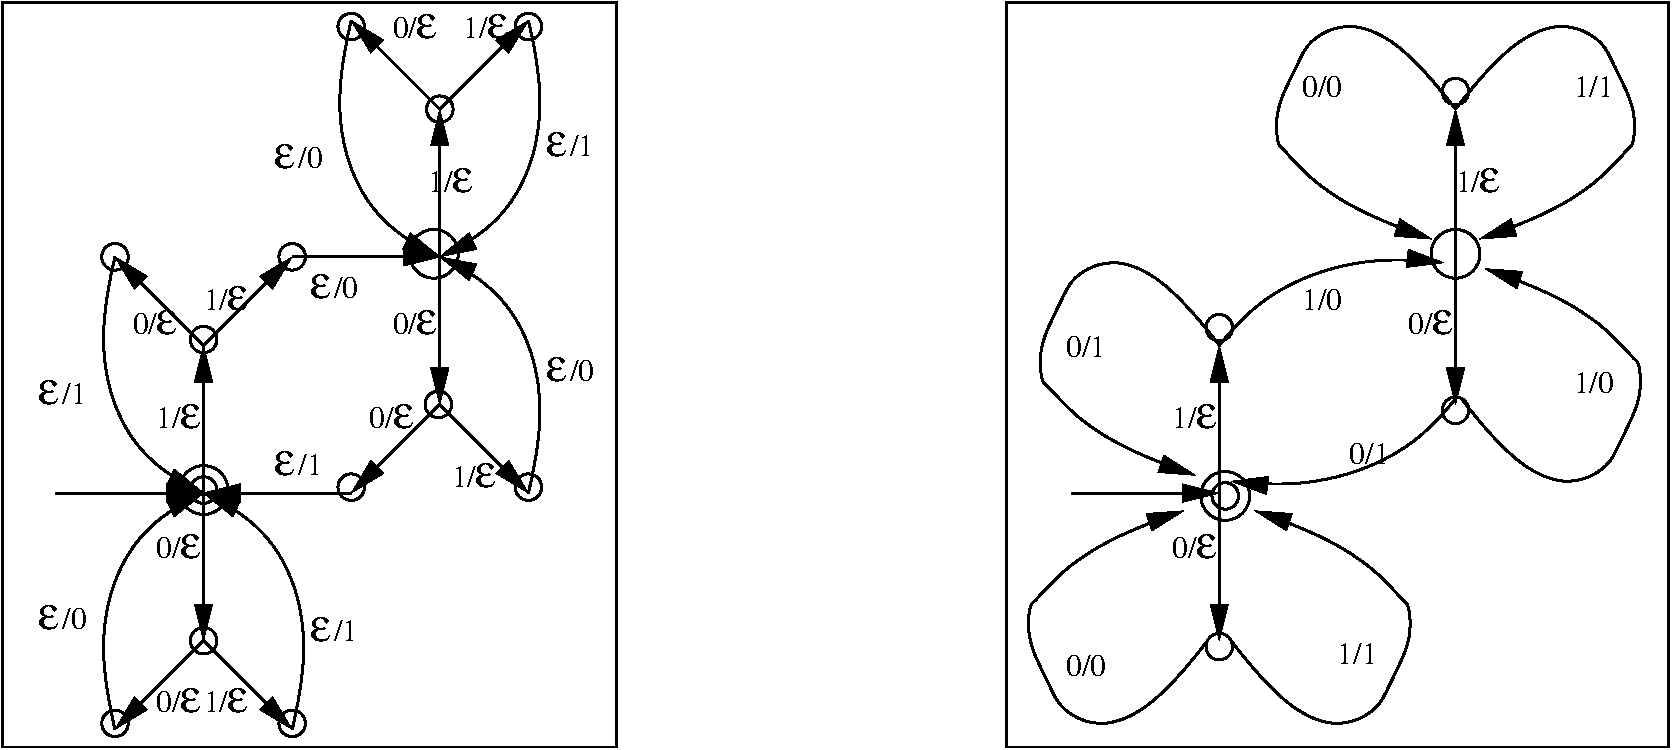
\includegraphics[%
%    width=0.7\linewidth,
%    keepaspectratio]{telop2}\end{center}
%  \caption{Two transducers that produce the sum of two numbers as
%    output \label{telop2}}
%  \end{figure}
%  
%  \paragraph{Selfie:}
%  \begin{itemize}
%  \item[]
%  Can a transducer also perform other arithmetic operations, like
%  subtraction or multiplication? Why or why not?
%  
%  Is the transducer output language regular?
%  
%  Can you write a transducer that outputs every third character of the
%  input string?
%  
%  Can you write a transducer that outputs all but every third character
%  of the input string?
%  
%  Can you write a transducer that outputs the input string in reverse
%  order?
%  
%  Can every regular language be the output language of a transducer?
%  \end{itemize}
%  
%  \subsection{Two-way finite automata}
%  
%  Sometimes, one calls a DFA a {\em one-way finite automaton}. The reason
%  is that one describes the DFA as a machine with an input tape on which
%  the input string resides: the machine has a reading head which is
%  initially above the first character of the string. At each transition,
%  the reading head moves one position to the right: always towards the
%  end of the string.
%  
%  A small adaptation of this automaton allows it to move in both
%  directions: you can adapt the definition of $\delta$ (see for instance
%  Chapter \ref{berekenbaarheid}: there, it is done for Turing
%  machines). What you get is a two-way finite automaton, or a 2DFA.
%  
%  About other classes of automata, we know that more freedom in how the
%  {\em memory} can be manipulated, leads to more powerful automata: to
%  fully appreciate this, you might have to wait until you learn about
%  PDA and LBA, but keep this in mind.
%  
%  Therefore, the question {\em is a 2DFA more powerful than a DFA?}, or
%  otherwise said {\em can a 2DFA recognise some non-regular languages?}
%  is relevant. What do you think?
%  
%  \project{hier kan zeker een mooi ding mee gedaan worden}
%  
%  
%  \subsection{B\"{u}chi automata}
%  
%  B\"{u}chi\footnote{Julius B\"{u}chi} automata are like NFAs, only you
%  feed them infinite strings: at no moment is the string finished.
%  That means that acceptance of a string by such an automata is
%  different from acceptance by an NFA:
%  
%  \begin{definition}
%  The infinite string is accepted by a B\"{u}chi automaton if the
%  sequence of states followed by the string passes by an accepting state infinitely many times.
%  \end{definition}
%  
%  Clearly that is something one can't try out or implement, but that is
%  not the purpose of B\"{u}chi automata: you use them to model a problem
%  (e.g. an infinitely repeating process, a protocol ...) and then prove
%  which strings satisfy the acceptance condition.
%  
%  Non-deterministic B\"{u}chi automata are strictly stronger than
%  deterministic B\"{u}chi automata: as an example, you could try to
%  build a B\"{u}chi automaton for the language $(a|b)^*b^\omega$. \footnote{$\omega$: look up transfinite numbers}
%  
%  \project{buchi automaten bestuderen ?}



\subsection{References}

\setlength{\intextsep}{0pt}
\begin{wrapfigure}[7]{r}{0.19\textwidth}
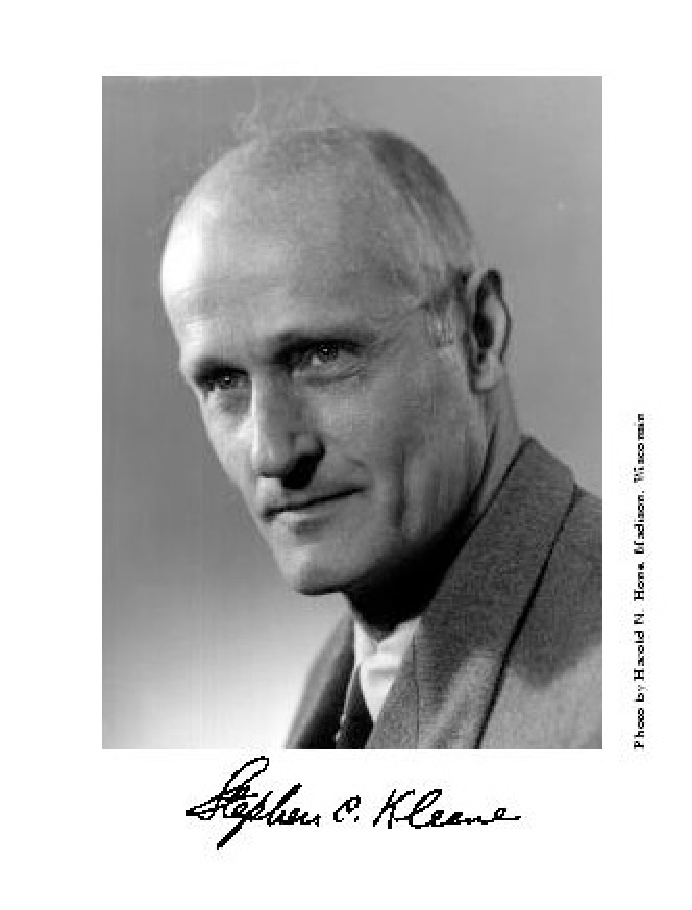
\includegraphics[width=.19\textwidth,keepaspectratio]{static/kleene}
\end{wrapfigure}


A lot of what you learned in this chapter has been developed by
Stephen Kleene: you might know him from fixpoint theorems. He also made contributions to logic, recursion theory, and intuitionism.

Modern texts on regular languages/expressions/machines do not always
follow the same order of presentation: in the previous sections, we
have shows that there is no chicken-and-egg problem, since all three
are equivalent. There is also a variety of small differences in the
basic definitions (e.g. whether $\delta$ needs to be total, 
% Vwhether there can be more than one accepting end state for the NFA 
\ldots): these
do not matter either.

The same diversity in definitions and approaches exists for other
languages and machines: we keep our mind open, focus on the
essentials, and make sure we know when things are basically
equivalent.



\paragraph{References:}

\begin{itemize}
\item
Dexter C. Kozen  {\em Automata and Computability}

\item
Peter Linz {\em An Introduction to Formal Languages and Automata}

\item
Michael Sipser {\em Introduction to the Theory of Computation}

\item
John E. Hopcroft, Rajeev Motwani, Jeffrey D. Ullman
{\em Introduction to Automata Theory, Languages, and Computation}

\item
Marvin Lee Minsky {\em Computation: Finite and Infinite Machines
(Automatic Computation)}
\end{itemize}

If all this gives you the hots, do not forget another important
book: {\em Regular algebra and finite machines}
% \footnote{The book is
%  not in the library, but if it interests you, pass by my office} 
by John Horton Conway - the same person of {\em The Game of Life} (it
appears later in this text) and other interesting issues (e.g. the
{\em Angels and Devils game}) that directly affect our understanding
of algorithmics.



\paragraph{Selfie:}
Below, we use the same alphabet for all languages, and it contains at
least $a$ and $b$.  We use the notation $\hat{s}$ to denote the string
with the same characters as $s$ but in reverse order. In each case,
formally write down the definition of L3. The question is always the
same: suppose L1 and L2 are regular languages, is L3 also regular?
\begin{itemize}
\item[]
L3 consists of strings obtained by merging strings of the same length
from L1 and L2 (also formally write down what merging means!)

L3 = $\widehat{L1}$

L3 consists of the strings with even length from L1

L3 consists of strings $s$ obtained by taking strings of even length
from L1, chopping such strings in two parts of equal length
as $s_1s_2$ and then concatenating $\widehat{s_1}$ with $s_2$

L3 consists of strings obtained by taking a string $s$ from L1 and
concatenating $s$ with $\hat{s}$

L3 has the strings from L1 in which every occurrence of $a$ is
replaced by $b$

L3 has the strings from L1 not in L2

L3 consists of the string from L1 from which the symbols on the even
places are taken out

$L3 = \{x|\exists y \in L2, xy \in L1\}$

$L3 = \{x|\exists y \in L2, yx \in L1\}$

\end{itemize}



%///////////////////////////////////////////////////////////////////////////////
\chapter{Context Free Languages and Grammars}\label{contextvrijelanguages}

%===============================================================================
\section{Basic Definitions}

Regular expressions provide one way to determine a language. One can
extend REs a little by allowing {\em abbreviations} for REs, so that
shorter descriptions of the language can be obtained. An abbreviation
gives a name to something, and when that name appears somewhere, you
can replace it with the thing it abbreviates (or a copy of it):
you now get an expression that does no longer contain the name, and
has the intended meaning. This means that

~~~~~~~~~Brackets \rpijl BracketsBrackets $|$ [Brackets] $|$ $\epsilon$

does not define an abbreviation: by replacing the name Brackets with
its meaning (the right side), you can not get rid of the
name. However, we can still use the above {\em rule} to define a
language. Such rules form a {\em context free grammar}. Before we
define that formally, here are a few examples:

\begin{example}
~~~
\begin{itemize}
\item
S \rpijl aSb

S \rpijl \eps

This grammar describes the strings of the form $a^nb^n$

\item

S \rpijl PQ

P \rpijl aPb

P \rpijl \eps

Q \rpijl cQd

Q \rpijl \eps

This grammar describes the strings of the form $a^nb^nc^md^m$


\item \label{statlabel}
Stat \rpijl Assign

Stat \rpijl ITE

ITE \rpijl If Cond Then Stat Else Stat

ITE \rpijl If Cond Then Stat

Cond \rpijl Id == Id

Assign \rpijl Id := Id

Id \rpijl a

Id \rpijl b

Id \rpijl c

\end{itemize}
\end{example}

Informally, a context free grammar (CFG) consists of rules; at the
left side in a rule, we see a nonterminal symbol; at the right side
we see a sequence of terminal and nonterminal symbols, and
\eps. There is also a start symbol.

One can use a CFG for generating strings, and also for checking
whether a string complies with the grammar. Generation is done by
making a derivation starting with the start symbol. The following is a
derivation using the first CFG example:

$~~~~~~~~~~S$ \rpijl $aSb$ \rpijl $aaSbb$ \rpijl $aabb$

The idea is: if a string contains a nonterminal, choose any
nonterminal X and replace it by the right hand side of a grammar rule
with X at the left. Start with the start symbol and continue until
there are only terminals.

We can represent essence of a derivation as a {\em syntax tree} or
{\em parse tree}: see Figure~\ref{parsetree1}.

\medskip
\begin{figure}[h]
\begin{center}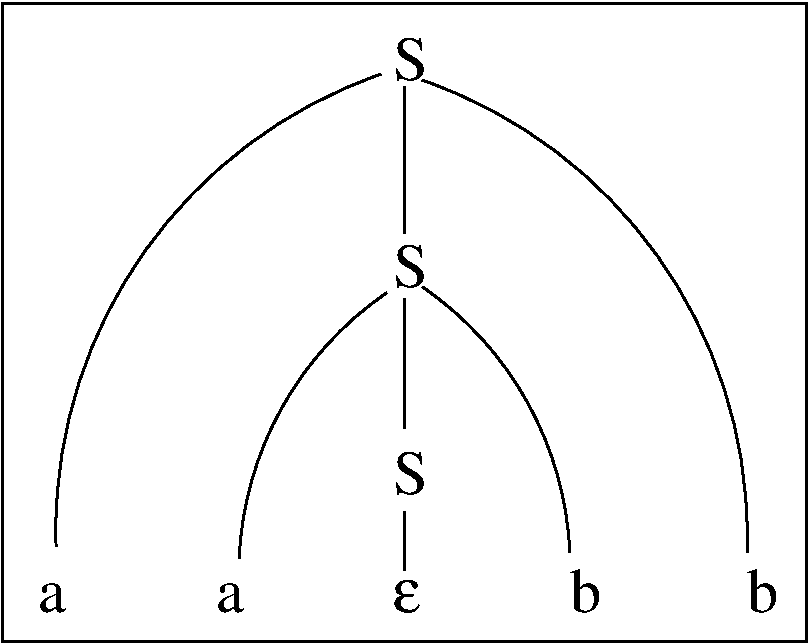
\includegraphics[%
  width=0.4\linewidth,
  keepaspectratio]{parsetree1}\end{center}
\caption{Syntax tree of aabb \label{parsetree1}}
\end{figure}

Clearly, the parse tree hides the order in which rules are applied
during the derivation.

We are now ready for more formal definitions.

\begin{definition}[Context Free grammar - CFG]
A context free grammar is a 4-tuple $(V,\Sigma,R,S)$ in which
\begin{itemize}
\item
$V$ is a finite set of nonterminal symbols (also named variables or
  nonterminals)
\item
$\Sigma$ is a finite alphabet of terminal symbols (terminals); $\Sigma
  \cap V = \emptyset$
\item
$R$ is a finite set of rules (or productions); a rule is a tuple
  consisting of one nonterminal and a string of elements from $V \cup
  \Sigma_\epsilon$; \\ we write the two parts of a rule with a \rpijl
  in between
\item
$S$ is the start symbol and $S \in V$
\end{itemize}
\end{definition}

It is often clear which are the terminals and which symbol is the
start symbol, and in such cases, we just mention the rules.

\begin{definition}[Derivation of a string, based on a CFG]
Let $(V,\Sigma,R,S)$ be a CFG.
A string $f$ over the alphabet $V \cup \Sigma_\epsilon$ is derived
from a string $b$ over $V \cup \Sigma_\epsilon$ using the CFG, if
there exists a finite sequence of strings $s_0, s_1, ..., s_n$
so that
\begin{itemize}
\item $s_0 = b$
\item $s_n = f$
\item $s_{i+1}$ is obtained from $s_i$ (for $i < n$) by replacing a nonterminal $X$ in
 $s_i$ by the right hand side of a rule in which
 $X$ occurs at the left.
\end{itemize}

We use the notation: $s_i \Rightarrow s_{i+1}$ and $b \Rightarrow^* f$
\end{definition}

\begin{definition}[The language determined by a CFG]
The language $L_{CFG}$ determined by the CFG $(V,\Sigma,R,S)$ is the
set of strings over $\Sigma$ that can be derived from $S$; or more
formally: $L_{CFG} = \{s \in \Sigma^* | S \Rightarrow^* s\}$.
\end{definition}

\begin{definition}[Context Free language - CFL]
A language $L$ is {\bf context free} if there exists a CFG so that $L
= L_{CFG}$
\end{definition}

Regarding CFLs, we intend to follow a similar path as for RegLans: we
define a new kind of machine and prove that the set of its accepted
languages coincides with the CFLs defined by CFGs. We study the
difference between deterministic and non-deterministic versions of
these machines; a pumping lemma for CFLs will be established; the
algebraic operations on CFLs are studied. We do not deal with
minimization: the reason why becomes clear in a later chapter
(remember this and get back to it!). We also treat an issue that was
a non-issue for RegLans: ambiguity.

\subsection{Ambiguity}

Consider the CFG Arit1\label{arit1label}
\begin{itemize}
\item Expr \rpijl Expr + Expr
\item Expr \rpijl Expr * Expr
\item Expr \rpijl a
\end{itemize}
Expr is the start symbol. Consider the string $a+a*a$: it belongs to
the language determined by Arit1. Below are two derivations of that
string (the substituted nonterminal is underlined whenever there is a
possible choice)

~~~~~$Expr \Rightarrow \underline{Expr} + Expr \Rightarrow a + Expr \Rightarrow a + \underline{Expr} * Expr$

$~~~~~~~~~~\Rightarrow a + a * Expr \Rightarrow a + a * a$

and

~~~~~$Expr \Rightarrow Expr + \underline{Expr} \Rightarrow Expr + Expr * \underline{Expr} \Rightarrow Expr + \underline{Expr} * a$

$~~~~~~~~~~\Rightarrow Expr + a * a \Rightarrow a + a * a$

In the former derivation, we always substituted the leftmost
nonterminal. In the latter always the rightmost one. But the parse
tree is in both cases the same (check that !). Those two derivations
are essentially the same, and this justifies that we consider only
leftmost derivations.

Consider now the following two leftmost derivations of $a+a*a$:



~~~~~$Expr \Rightarrow Expr + Expr \Rightarrow a + Expr \Rightarrow a + Expr * Expr$

$~~~~~~~~~~\Rightarrow^* a + a * a$

and

~~~~~$Expr \Rightarrow Expr * Expr \Rightarrow Expr + Expr * Expr  \Rightarrow a + Expr * Expr$

$~~~~~~~~~~\Rightarrow^* a + a * a$

or in terms of their parse trees: see Figure~\ref{ambi1}:

\begin{figure}[h]
\begin{center}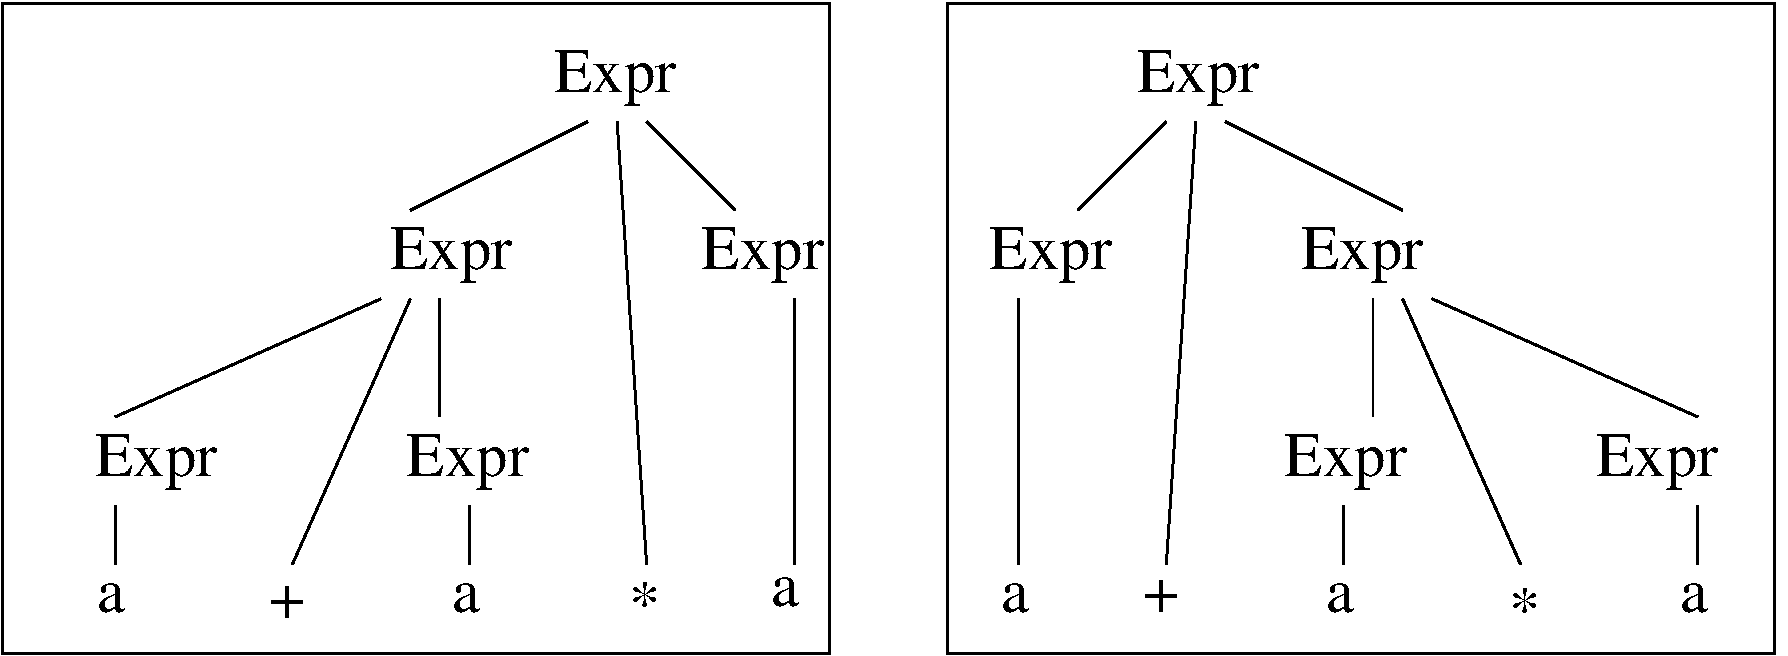
\includegraphics[%
  width=0.7\linewidth,
  keepaspectratio]{ambi1}\end{center}
\caption{Two parse trees for $a+a*a$\label{ambi1}}
\end{figure}

The string a+a*a seems to have more than one leftmost derivation and
more than one parse tree: the (meaning of the) string is ambiguous.
We say that grammar Arit1 is ambiguous because there exist ambiguous
strings in $L_{Arit1}$ w.r.t. Arit1. A priori, it is unclear whether
for the same language there exists also a non-ambiguous grammar.

\begin{definition}[Equivalence of CFGs]
Two context free grammars $CFG1$ and $CFG2$ are equivalent if

$~~~~~~~~~~~L_{CFG1} = L_{CFG2}$
\end{definition}

You should be able to prove that this defines an equivalence relation
on the CFGs.

We define a different CFG Arit2\label{arit2label}:

\begin{itemize}
\item Expr \rpijl Expr + Term
\item Expr \rpijl Term
\item Term \rpijl Term $*$ a
\item Term \rpijl a
\end{itemize}

Convince yourself that Arit1 and Arit2 are equivalent.

You can also check that $a+a*a$ has only one leftmost derivation:


$Expr \Rightarrow Expr + Term \Rightarrow Term + Term \Rightarrow a + Term$

$~~~~~~~~~~\Rightarrow a + Term * a \Rightarrow a + a * a$


and even better, every string in its language has exactly one parse
tree for Arit2. We say: Arit2 is a non-ambiguous grammar.


Not every CFL has a non-ambiguous CFG: such a CFL is named {\em
  inherently ambiguous}. Here is an example of such a language:
%
 $\{a^nb^mc^m| n,m \geq 0\} \cup \{a^nb^nc^m| n,m \geq 0\}$. The proof that it is
inherently ambiguous can be found in the Hopcroft-Motwani-Ullman book,
but you should be able to prove that the language is context free.
We get back to ambiguity later.

A final note on notation: if a nonterminal occurs at the left side of
more than one rule, we can cluster those rules. For instance, grammar
Arit2 can be written as:
\begin{itemize}
\item Expr \rpijl Expr + Term $|$ Term
\item Term \rpijl Term $*$ a $|$ a
\end{itemize}




\subsection{Special forms of CFGs}

Often, it is convenient to have grammars of a restricted form, but
without excluding any CFLs. Here is such a form.

\begin{definition}[Chomsky Normal Form]
A CFG is in Chomsky Normal Form if every rule has one of the following
forms
\begin{enumerate}
\item A \rpijl BC  (with A,B,C nonterminals; B,C are different from the start symbol)
\item A \rpijl $\alpha$ (with $\alpha$ a terminal)
\item $S$ \rpijl $\epsilon$ (with $S$ the start symbol)
\end{enumerate}
\end{definition}

Some textbooks do not include the rule $S$ \rpijl $\epsilon$: such a grammar
cannot derive the empty string.

\begin{theorem} \label{chomskynormalform}
For each CFG there exists an equivalent CFG in Chomsky Normal Form.
\end{theorem}
\begin{proof}
The proof is constructive, a bit long but not difficult. We start from
a given CFG and transform it in little steps to Chomsky Normal Form
while retaining equivalence.

\begin{enumerate}
\item[{\bf 1.}] We start by making sure that there is a start symbol
  that never occurs at the right of a rule: if $S$ is the start symbol
  in the given grammar, replace it everywhere by a new nonterminal
  (say X) and add the rule $S \rightarrow X$

\item[{\bf 2.}] We now try to satisfy the third requirement of the
  definition of Chomsky Normal Form:

suppose there exist rules ${\cal E} = A \rightarrow \epsilon$ and
${\cal R} = B \rightarrow \gamma$ with A occurring in $\gamma$; we
define the set of rules $V({\cal E},{\cal R})$ of the form
%
$B \rightarrow \eta$ in which $\eta$ is obtained from $\gamma$ by deleting any combination of occurrences of A in $\gamma$.

Then transform the grammar as follows:

\begin{itemize}
\item[]
while there exist rules ${\cal E} = A \rightarrow \epsilon$ and
${\cal R} = B \rightarrow \gamma$ with A occurring in $\gamma$ and
such that $V({\cal E},{\cal R})$ contains {\em new} rules, add
$V({\cal E},{\cal R})$ to the grammar
\end{itemize}
Make sure you understand that this ends!

Then delete from the grammar all rules of the form $A \rightarrow
\epsilon$, except if $A = S$: that is potentially the only rule
deriving \eps.

Make sure you understand that the resulting grammar still defines the
same language: reasoning on the derivations can help.



\item[{\bf 3.}] We now want to get rid of the rules of the form
$A \rightarrow B$ with A and B nonterminals. For a rule of the form
${\cal E} = A \rightarrow B$ and a rule of the form ${\cal R} = B
  \rightarrow \gamma$, define the rule $U({\cal E},{\cal R}) = A
  \rightarrow \gamma$.

\begin{itemize}
\item[]
while there exists rules of the form ${\cal E} = A \rightarrow B$
and ${\cal R} = B \rightarrow \gamma$, and $U({\cal E},{\cal R})$ is a
new rule, add $U({\cal E},{\cal R})$ to the grammar
\end{itemize}
Make sure you understand that this ends!



Then remove from the grammar all rules of the form $A \rightarrow B$.

Make sure you understand that the resulting grammar still defines the
same language: reasoning on the derivations can help.


\item[{\bf 4.}] There are now 3 types of rules:
\begin{enumerate}
\item
$A \rightarrow \gamma$ in which $\gamma$ has exactly two nonterminals:
  they can stay

\item
$A \rightarrow \gamma$ in which $\gamma$ has at least two symbols;
  replace each terminal $a$ by a new nonterminal $A_a$, and add the
  rule $A_a \rightarrow a$

\item
possible $S \rightarrow \epsilon$: it can stay

\end{enumerate}
Once more, make sure you understand that this ends and that the
language remains the same!


\item[{\bf 5.}] rules of the form $A \rightarrow X_1X_2...X_n$ with $n
  > 2$ are now replaced by \\ $A \rightarrow X_1Y_1$, ~~$Y_1 \rightarrow
  X_2Y_2$, ~~..., ~~$Y_{n-2} \rightarrow X_{n-1}X_n$

\end{enumerate}

... and by now, you know what to do.

Do we have a grammar in Chomsky Normal Form now?
\end{proof}

The Chomsky Normal Form has several advantages: we can see immediately
whether the language contains the empty string; every parse tree is
(almost) a full binary tree (that will turn out to be handy in the
pumping lemma). On top of that, every derivation of a string of
length $n > 0$ has length $2n-1$: that will be useful when we study
decision problems related to CFLs.

There exist other normal forms for CFGs. As an example, the
Greibach\footnote{Sheila Greibach} normal form restricts grammars to
rules of the form
\begin{itemize}
\item A \rpijl aX
\item $S$ \rpijl \eps
\end{itemize}
in which X is a (possibly empty) sequence of nonterminals and $a$ a
terminal. Now, derivations are no longer than the
string!\footnote{Careful, do not conclude that one can make the
  derivation of a given string in linear time!} Try proving the
analogue of the theorem on page \pageref{chomskynormalform} but now
for the Greibach normal form.

\paragraph{Selfie:}
\begin{itemize}
\item[]
Prove that a derivation of a string of length $n > 0$ from a grammar
in Chomsky normal form has length $2n-1$.

Prove that a derivation of a string of length $n > 0$ from a grammar
in Greibach normal form has length $n$.

Can you use the transformation to Chomsky normal form to understand
that every (pure) Prolog program can be transformed to an equivalent
Prolog program with zero or two goals in each clause body?
\end{itemize}



\section{The Pushdown Automaton}

An FSA has no memory besides its state, and since there is only a
finite number of them, an FSA can not count in an unlimited way. As a
result, it is incapable of determining lots of interesting
languages. The next machine we introduce - the pushdown automaton
(PDA) - has an unlimited memory, but it can use that memory in a very
limited way only: the memory is organised as a stack, and at any given
moment, only the top of the stack can be inspected or changed. The
latter happens by adding an element (push) or deleting it (pop).
As with the regular automata, we use PDAs as a means to decide whether
a string is accepted: successive characters from the string are
consumed, and based on the current state and the current top of the
stack, the machine goes to a new state, and possibly changes the top
of the stack. Just as with regular automata, we define the PDA from
the start as non-deterministic.

\begin{definition}[The pushdown automaton]
A pushdown automaton is a 6-tuple
$(Q,\Sigma,\Gamma,\delta,q_s,F)$ in which
\begin{itemize}
\item $Q$ is a finite set of states
\item $\Sigma$ is a finite input alphabet
\item $\Gamma$ is a finite stack alphabet
\item $\delta$ is a transition function with signature
%
$Q \times \Sigma_\epsilon \times \Gamma_\epsilon \rightarrow {\cal P}(Q \times  \Gamma_\epsilon)$
\item $q_s$ is the start state
\item $F \subseteq Q$ is the set of (accepting) end states
\end{itemize}
\end{definition}

This definition does not specify how a PDA works. Let us first look at
a graphical representation of a PDA, similar to the graphical
representation for an FSA. As an example, we take PDA
$(Q,\Sigma,\Gamma,\delta,q_s,F)$ with

\begin{itemize}
\item $Q = \{q_s, q_f, x, y\}$
\item $F = \{q_f\}$
\item $\Sigma = \{a,b,c\}$
\item $\Gamma = \{m, \$\}$
\end{itemize}

The $\delta$ can be seen in Figure~\ref{pda2}.

\medskip
\begin{figure}[h]
\begin{center}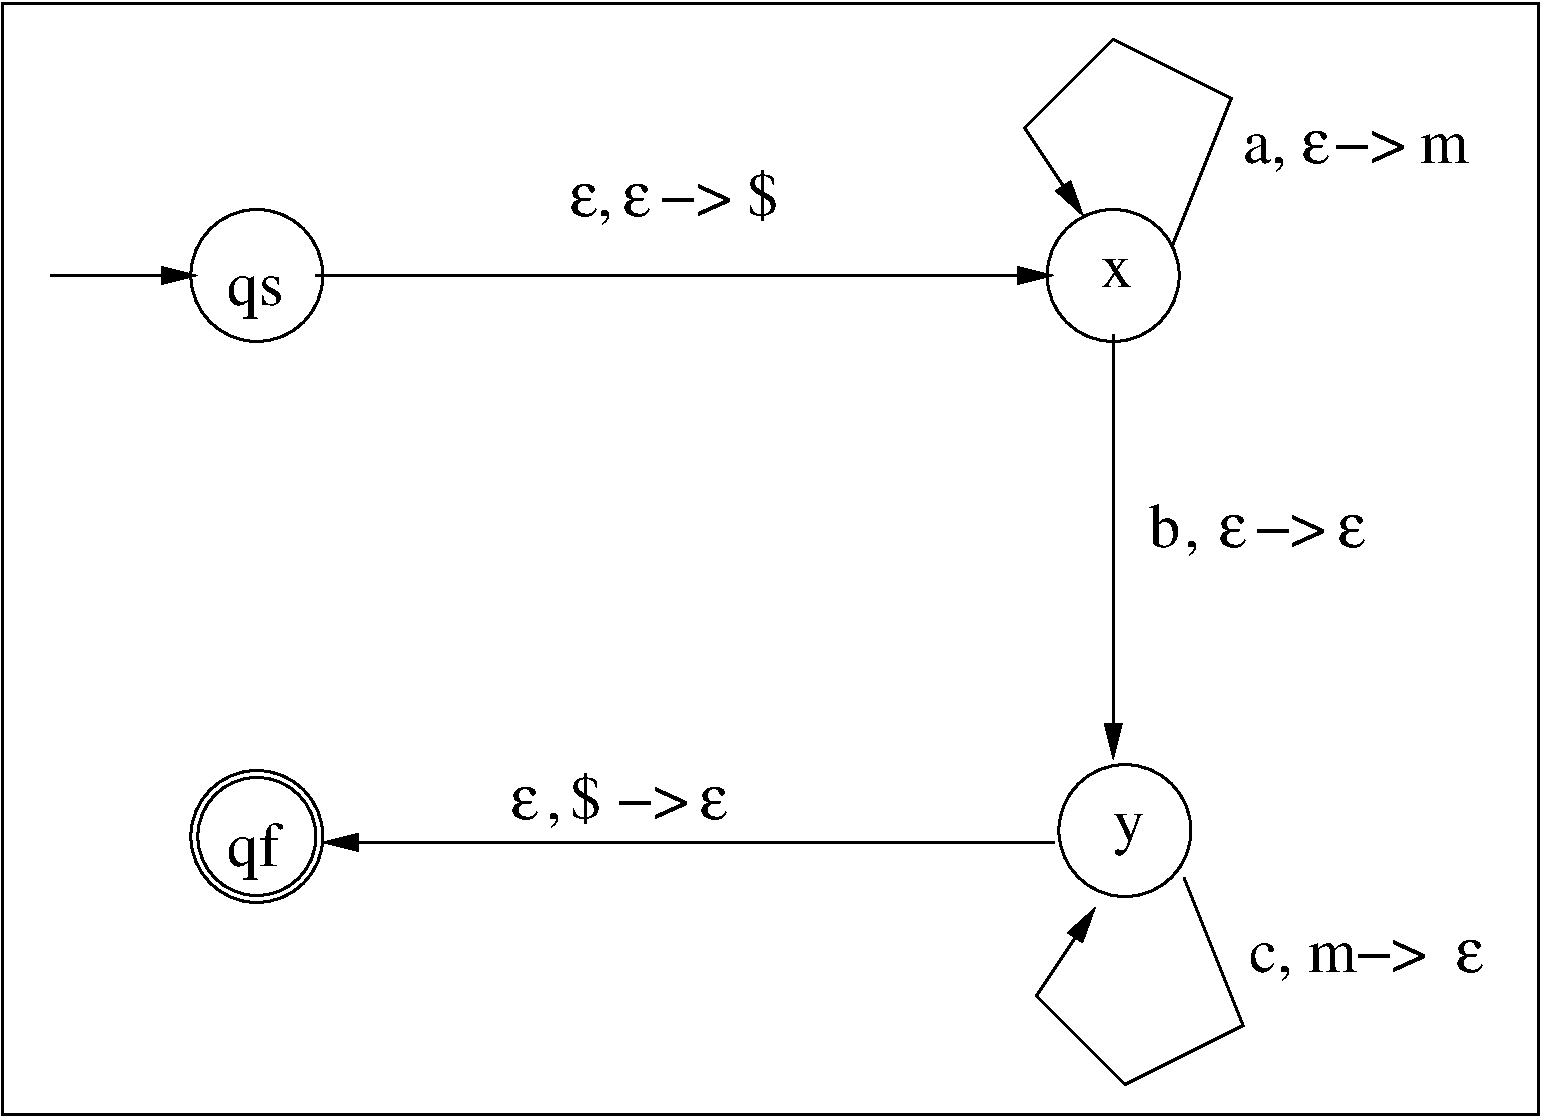
\includegraphics[%
  width=0.6\linewidth,
  keepaspectratio]{pda2}\end{center}
\caption{A pushdown automaton\label{pda2}}
\end{figure}

The meaning of an edge label like $\alpha,\beta \rightarrow \gamma$ is

\begin{itemize}
\item if $\alpha$ is the first symbol of the current string
\item and $\beta$ is at the top of the stack
\item then follow the edge and
\begin{itemize}
\item remove $\alpha$ from the string
\item remove $\beta$ from the stack
\item put $\gamma$ on the stack
\end{itemize}

\end{itemize}

$\alpha$, $\beta$ and $\gamma$ may be $\epsilon$. For $\alpha$ this
means: do not take the beginning of the string into account; for
$\beta$ it means: do not take top of the stack into account; for
$\gamma$: do not push anything.

As you see, the labels specify $\delta$.

The first time we arrive at $y$ after starting in $q_s$ with string
$a^2bc^2$ and an empty stack, the stack contains $mm\$$, and the string
is reduced to $c^2$. Applying $\delta$ two more time exhausts the
string and a final application of $\delta$ brings us in the end
state. We say: $a^2bc^2$ is accepted by the PDA, or $a^2bc^2$ is in
the language determined by the PDA. Here is the formal definition:

\begin{definition}[A string accepted by a PDA]
A string $s$ is accepted by a PDA if $s$ can be split in parts
$w_i$, i= 1..m ($w_i \in \Sigma_\epsilon$), and there exist states
 $q_j$, j= 0..m, and stacks $stack_k$, k=0..m ($stack_k
\in \Gamma^*$), so that
\begin{itemize}
\item $stack_0 = \epsilon$  (the stack is empty at the start)
\item $q_0 = q_s$ (the first state is the start state)
\item $q_m \in F$ (we arrive in an end state with an empty string)
\item $(q_{i+1},y) \in \delta(q_i,w_{i+1},x)$ in which  $x,y \in
\Gamma_\epsilon$ and

$stack_i = xt,~~stack_{i+1} = yt$ with $t \in \Gamma^*$
\end{itemize}
\end{definition}

The last bullet indicates that the transitions follow $\delta$.

\paragraph{Caveat:}

Acceptance as defined above, does not take the contents of the stack
into account at the moment of arriving in an end state: the string
being empty is enough. There exist many alternative definitions for
the PDA: some allow to push more than one symbol during a transition;
some define acceptance as {\em the string and the stack are both
  empty}, in which case the notion of end state is not even needed;
some define acceptance as {\em the string and the stack are both empty
  and we are in $F$}; some require that at each transition either a
symbol is pushed or popped, but not both; some have only one end state
\ldots All these are equivalent in terms of the set of languages that can
be determined by these machines. So, do not get too hung up on the
exact definition, but better stick to a particular one while doing a
proof or an exercise.

\project{ivm equivalentie van die dingen - misschien ook minimisatie
NFA/MN voor NFA}

\begin{definition}[The language determined by a PDA]
The language determined by a PDA is the set of strings accepted by the
PDA.
\end{definition}

Clearly, the language $\{a^nbc^n|n \geq 0\}$ is determined by a PDA:
Figure~\ref{pda2} shows the implementation. Strings like aabc are not
accepted.


Switching between alternative definitions of the PDA can be
tricky. Look at the PDA defined in Figure~\ref{pda1}: at first sight
you might think it accepts the same language as in Figure~\ref{pda2},
but is that really so?

\begin{figure}[h]
\begin{center}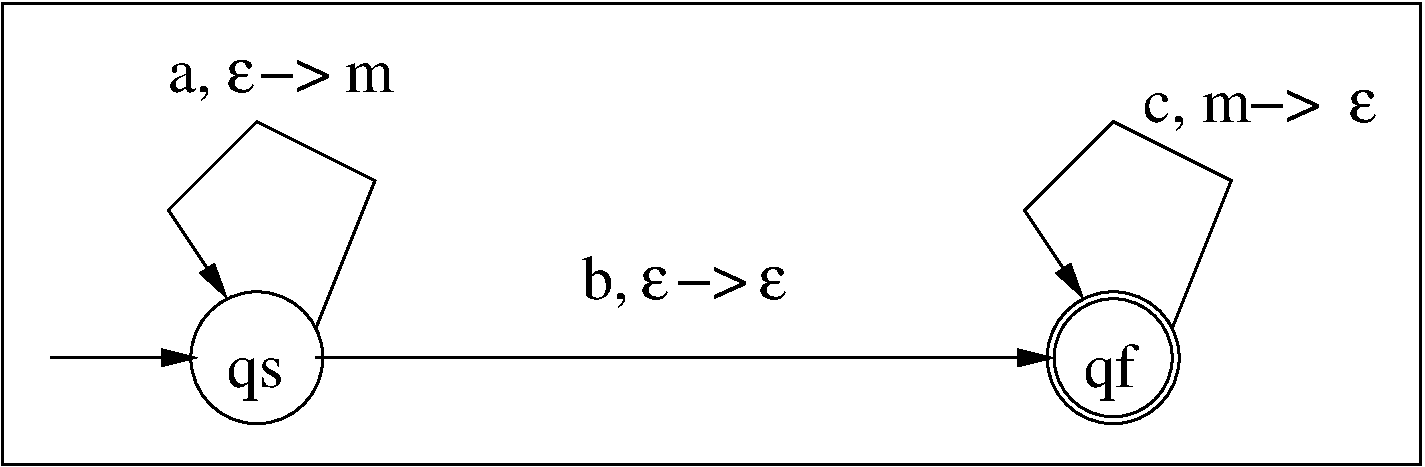
\includegraphics[%
  width=0.6\linewidth,
  keepaspectratio]{pda1}\end{center}
\caption{Another pushdown automaton for the same language?\label{pda1}}
\end{figure}

It is only true if you define acceptance for this PDA as {\em arrive
  in the end state with an empty stack and string}. So you see that
the details of the definition matter for a given PDA. On the other
hand, the details of the definition change nothing to the class of
languages determined by PDAs.



\section{Equivalence of CFG and PDA}

We want to prove

\begin{theorem}
Every PDA determines a CFL and every CFL is determined by a PDA.
\end{theorem}
\begin{proof}
There are clearly two parts in this theorem. We prove the first part
in the lemma on page \pageref{equicfgpda1}, and the second part in the lemma on page \pageref{equicfgpda2}.
\end{proof}

We first need some preparatory work and an example.

We mentioned before that allowing PDAs to push more than one symbol
during a transition does not change the power of PDAs: if you haven't
done that yet, this is a good moment to prove it! We use this feature
because it makes the description of the example much shorter.



\begin{figure}[h]
\begin{center}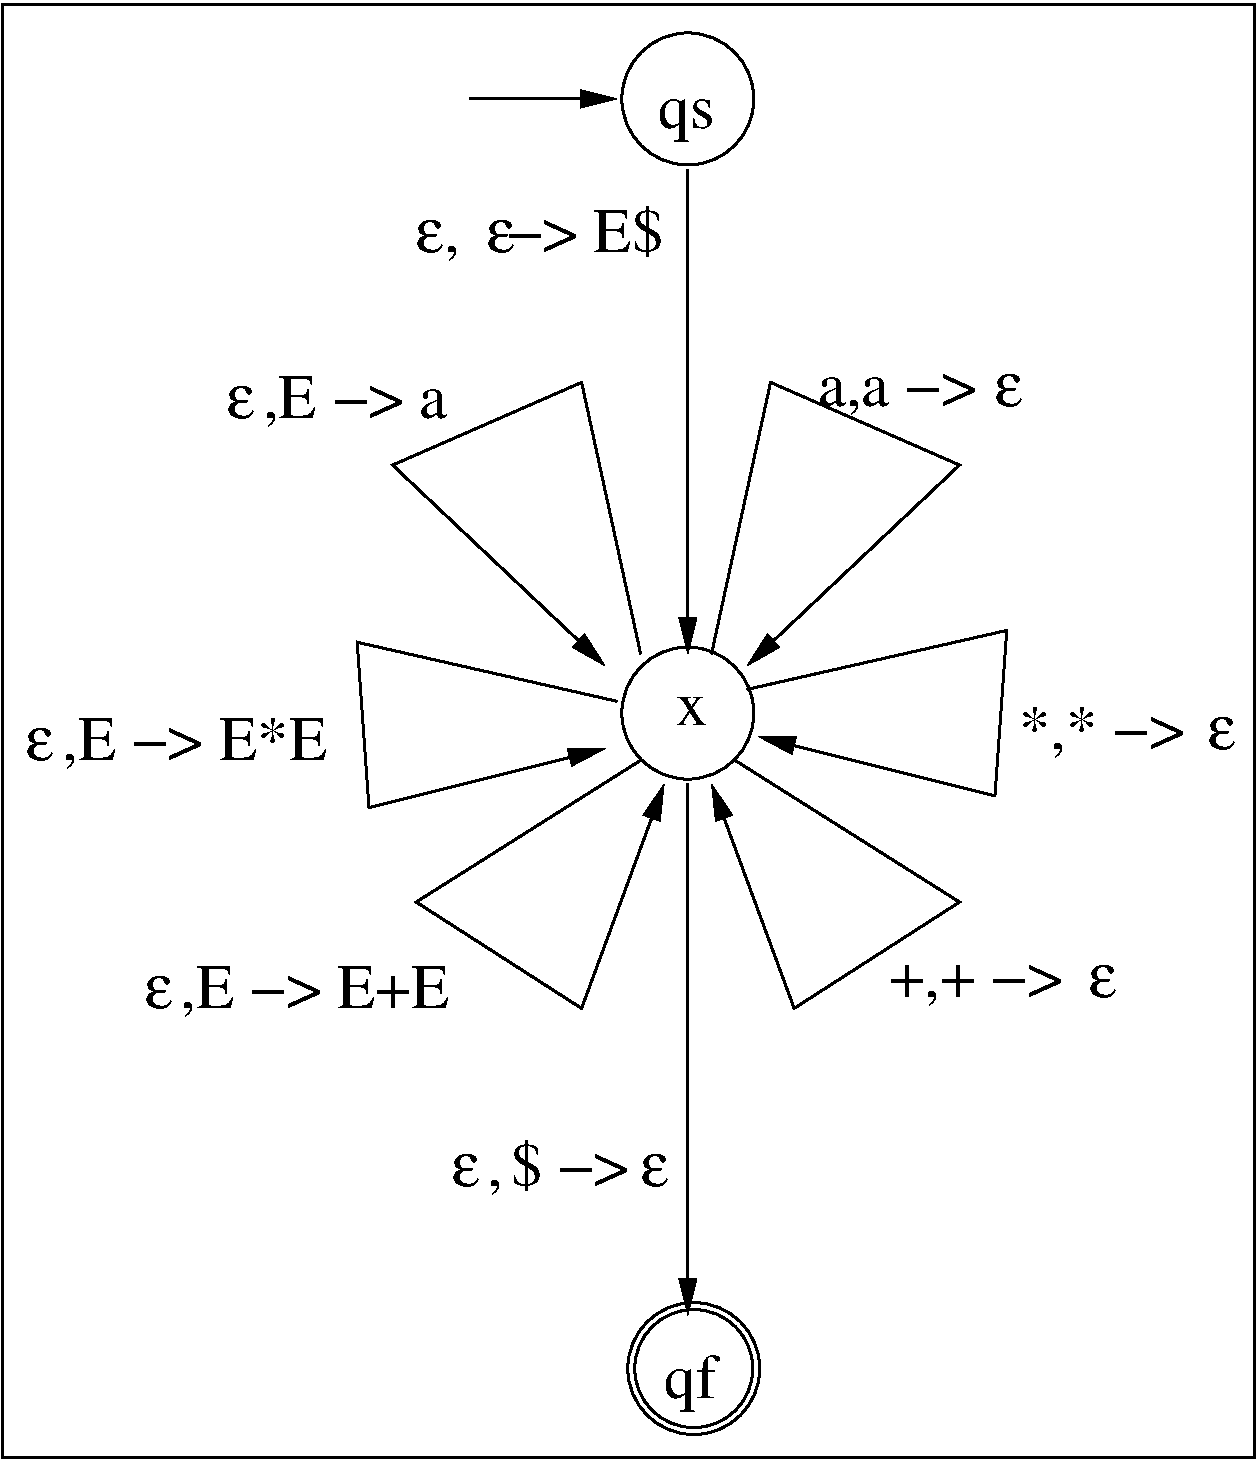
\includegraphics[%
  width=0.45\linewidth,
  keepaspectratio]{pda3}\end{center}
\caption{A PDA derived from Arit1\label{pda3}}
\end{figure}

\begin{example}
Consider again the CFG Arit1 of page \pageref{arit1label}
\begin{itemize}
\item E \rpijl E + E~~~~~~~E \rpijl E * E~~~~~~~E \rpijl a
\end{itemize}
with E the start symbol. Now look at the PDA in Figure~\ref{pda3}.

This PDA has a bit more symmetry than you would get starting from
another CFG. Still, it is constructed in a systematic way as follows:

%
\begin{itemize}
\item it has 3 states: the start state $q_s$, the end state $q_f$, and
 one {\em helper} state $x$

\item there is one edge from $q_s$ to $x$: it ignores the string and
  the stack; it pushes a marker \$ and the start symbol on the stack

\item there is one edge from $x$ to $q_f$: it consumes nothing from
  the string and it takes the marker \$ from the stack

\item all other edges connect $x$ with $x$; their labels correspond to
\begin{itemize}

\item the symbols of $\Sigma$: for each $\alpha \in \Sigma$, there is
  an edge with label $\alpha,\alpha \rightarrow \epsilon$; the meaning
  of these edges is: if the top of the stack is the same symbol as the
  first symbol of the string, consume both

\item the grammar rules: for each rule $X \rightarrow \gamma$ there is
  an edge with label $\epsilon, X \rightarrow \gamma$; the meaning
  of these edges is: if the top of the stack is a nonterminal X,
  replace it by $\gamma$; $\gamma$ is a sequence of terminals and
  nonterminals
\end{itemize}

\end{itemize}
\end{example}

\paragraph{Selfie:} Describe exactly $\Sigma$ and $\Gamma$ for this PDA.


We use the PDA to parse the string $a+a*a$: Table~\ref{parsing1} shows the
stack and the string during parsing. Note that when we push the
sequence of symbols XYZ, we actually want them in reverse order, so the representation of the stack is a string to which we add at the front (without reversing the XYZ) and from which we pop from the left.


\begin{table}[ht]
\center
\begin{tabular}{|r|r|r|}
\hline
string     &  stack      & state \\ \hline
a+a$*$a      & $\epsilon$   & $q_s$   \\
a+a$*$a      &   E\$        & $x$     \\
a+a$*$a      &   E$*$E\$       & $x$       \\
a+a$*$a      &   E+E$*$E\$     & $x$       \\
a+a$*$a      &   a+E$*$E\$     & $x$       \\
 +a$*$a      &    +E$*$E\$     & $x$       \\
  a$*$a      &   E$*$E\$       & $x$       \\
  a$*$a      &   a$*$E\$       & $x$       \\
   $*$a      &    $*$E\$       & $x$       \\
    a      &     a\$       & $x$       \\
$\epsilon$ &      \$       & $x$       \\
$\epsilon$ & $\epsilon$   & $q_f$    \\
\hline
\end{tabular}
\caption{Parsing $a+a*a$} \label{parsing1}
\end{table}
The above parse is a leftmost derivation. It is not necessarily
unique: choose E+E instead of E$*$E at the second step, and you will
still accept.

Is it possible that you get stuck? Try E*E instead of E$+$E at the 3rd
step, and you will see. Does that indicate a problem?

Convince yourself that $L_{Arit1}$ equals the set of strings accepted
by the PDA in Figure~\ref{pda3}.

We can generalize the example to the following lemma:


\begin{lemma} \label{equicfgpda1}
The construction of a PDA from a CFG as described above, results in
a PDA that accepts the language $L_{CFG}$.
\end{lemma}
\begin{proof}
You can check that there is a one-to-one correspondence between a
derivation of string $s$ using the CFG, and an accepting execution of the PDA for $s$.
\end{proof}

The above construction results in a nondeterministic PDA whenever the
CFG has two (or more) rules for a particular nonterminal. This might
give the impression that the grammar is ambiguous, but that's not true: grammar
Arit2 on page \pageref{arit2label} also results in a nondeterministic
PDA, but Arit2 is not ambiguous. Still, you could wonder about the
following questions
\begin{itemize}
\item
if L has a deterministic PDA, then L is not ambiguous
\item
a nondeterministic PDA can be transformed to an equivalent
deterministic one
\end{itemize}


The construction of a PDA from a CFG is easy: you need only 3
states and there is a very uniform description of its transitions.
The reverse direction - from a PDA to a CFG - is disappointingly more
complicated, partly because not every PDA has 3 states. 
% Also, our
% DFA-to-RE method using the GNFA seems not to work here (why not?).


We will assume that the PDA has a particular form
\begin{itemize}
\item there is only one end state
\item the stack is being emptied before we arrive there
\item each transition pops one symbol from the stack, or pushes one
  symbol onto the stack, but not both
\end{itemize}
We mentioned this form earlier - now is a good time to prove that it
is not restrictive.


\subsection{Construction of a CFG $(V,\Sigma,R,S)$ from a PDA
$(Q,\Sigma,\Gamma,\delta,q_s,\{q_f\})$:}
\begin{itemize}
\item $V = A_{p,q}$ with $p, q \in Q$
\item $S = A_{q_s,q_f}$
\item $R$ has 3 parts
\begin{itemize}
\item rules of the form $A_{p,p} \rightarrow \epsilon$ for each $p \in Q$
\item rules of the form $A_{p,q} \rightarrow A_{p,r}A_{r,q}$ for each
  $p, q, r \in Q$
\item rules of the form $A_{p,q} \rightarrow aA_{r,s}b$ in which

$p, q, r, s \in Q, ~~
a,b \in \Sigma_\epsilon, ~~
t \in \Gamma,~~
(r,t) \in \delta(p,a,\epsilon),~~
(q,\epsilon) \in \delta(s,b,t)$
\end{itemize}

\end{itemize}

The intuition behind this construction is this: the strings that bring
you in the PDA from state p with an empty stack to state q with an empty
stack, are exactly the strings generated by the nonterminal $A_{p,q}$.

\begin{lemma} \label{equicfgpda2}
The above construction of a CFG from a PDA preserves the language.
\end{lemma}
\begin{proof}
We don't do the proof this year :-)
\end{proof}


\paragraph{Consequence I:} a language accepted by a PDA is context free.

\paragraph{Consequence II:} every regular language is context free. The reason is that an FSA is also a PDA: it just ignores the stack.

\paragraph{Selfie:}
Another way to understand that regular languages are context free:
construct a CFG for the given regular language.

\paragraph{To conclude (for now)} we mention two more theorems
that provide better understanding of the structure of CFLs.

A theorem by Chomsky-Sch\"{u}tzenberger states that every CFL is
essentially the intersection of a regular language with a {\em
  Dyck\footnote{Walther von Dyck} language}: a Dyck language consists
of balanced strings of parentheses, possibly more than one.

Parikh's theorem can best be formulated using the transformation
$Ord$ of a language: you obtain Ord($s$) by putting the symbols of $s$
in alphabetic order. As an example $Ord(bacabbc) = aabbbcc$. Parikh
states: for each CFL L, there exists a regular language R so that
$Ord(L) = Ord(R)$. I.e. apart from the order of the symbols in their
strings, regular and context free languages are the same!

\project{Parikh of Chomsky-Sch\"{u}tzenberger uitwerken}


\section{A Pumping Lemma for Context Free Languages}\label{pompcfl}

\begin{theorem}
For every context free language L, there exists a number p (the
pumping length), so that for each string $s \in L$ with $|s| \geq p$,
there exists a partition of $s$ in 5 pieces u,v,x,y and z from
$\Sigma^*$ so that $s$ = uvxyz
\begin{enumerate}
\item $\forall i \geq 0: uv^ixy^iz \in L$
\item $|vy| > 0$
\item $|vxy| \leq p$
\end{enumerate}
\end{theorem}
\begin{proof}
We use once more the pigeon hole principle, now on the parse tree for
strings that are long enough. Consider a CFG in Chomsky normal form
for L. Let $n$ be the number of nonterminals.

If $s \in L$, it has a parse tree. By deleting the
leaves from that tree, we get a full binary tree - because of the Chomsky normal
form. The height of this tree is at least $log_2(|s|)$, so the longest
(simple) path from the root has at least $log_2(|s|) + 1$ vertices. If
we chose $s$ long enough, $log_2(|s|) + 1 > n$ and consequently, on
this longest path at least one nonterminal - say X - is
repeated. Consider the occurrence of X that is closest to the root,
and denote it by $X_2$; denote by $X_1$ the closest re-occurrence on
that path. Note that X does not equal S
(why?). Figure~\ref{parsetree2} illustrates the situation. From the
parse tree we can construct a derivation of which we show only some
steps:


$~~~~~~~~S \Rightarrow^* uX_2z \Rightarrow^* uvX_1yz \Rightarrow^* uvxyz$ (a)

In this derivation u,v,x,y,z are strings from $\Sigma^*$ and moreover
v and y are not both empty, because that would mean that X could
derive itself, which is impossible because of the Chomsky normal form.

Since (a) is a good derivation,


$~~~~~~~~S \Rightarrow^* uX_2z \Rightarrow^* uxz$

is too, and



$~~~~~~~~S \Rightarrow^* uXz \Rightarrow^* uvXyz \Rightarrow^* uvvxyyz$


as well and \ldots

So we already have obtained (1) and (2) from the theorem if we take strings longer than $2^{(n-1)}$: that is our pumping length p.


We now prove (3): vxy is derived from X with a parse tree smaller than
$n$, so it has at most $2^{n-1}$ leaves which correspond exactly with
vxy. Figure~\ref{parsetree2} once more illustrates this.
\end{proof}

\begin{figure}[h]
\begin{center}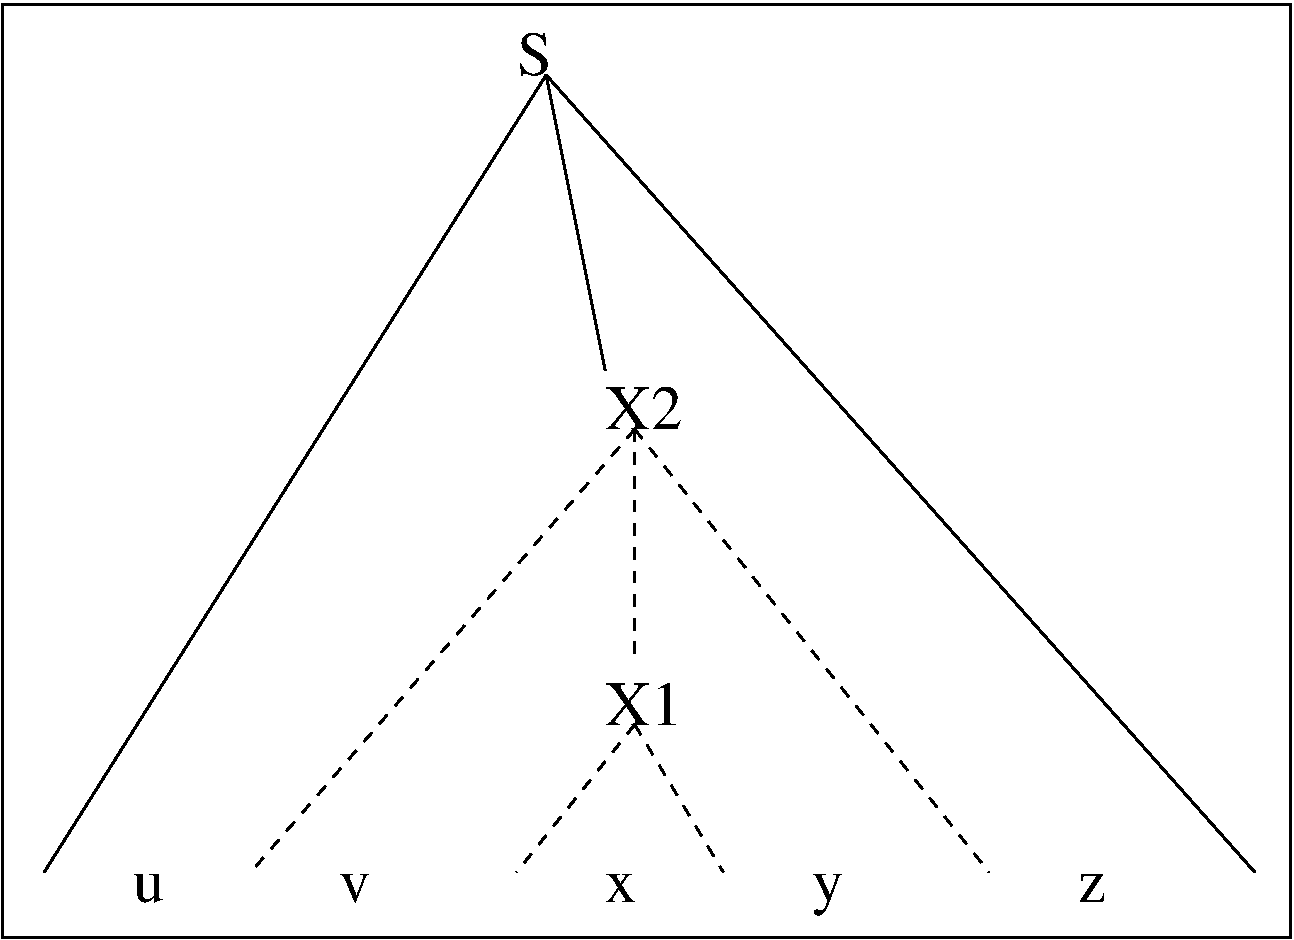
\includegraphics[%
  width=0.35\linewidth,
  keepaspectratio]{parsetree2}\end{center}
\caption{The parse tree with the repeating nonterminal
  X \label{parsetree2}}
\end{figure}


\subsection{Using the pumping lemma for CFLs}\label{voorbeeldpompcfl}

Consider the language $L = \{a^nb^nc^n | n \geq 0\}$. Suppose that
there exists a pumping length p. We must take a string $s$ longer than
p, say $s = a^pb^pc^p$.  Suppose that $s = uvxyz$ with $|vy| >
0$. Then there are two possibilities:
\begin{enumerate}
\item
v has the form $\alpha^k$ and y has the form $\beta^l$ and
$\alpha$ and $\beta$ are in $\{a,b,c\}$; in this case we have that
$k+l > 0$. Now, $uv^2xy^2z$ does not have the same number of a's, b's
and c's

\item
v or y contains more than one symbol from $\{a,b,c\}$; then $v^2$ or
$y^2$ contains those symbols in the wrong order, so $uv^2xy^2z$ does not belong to the language

\end{enumerate}

As a consequence, $s$ can not be pumped and so L is not context free.



\section{Further Discussion}

\subsection{An Algebra of CFLs?}

The union of two CFLs determined by CFGs $CFG_1$ and $CFG_2$ can be
described easily by the following construction: first make sure the two CFGs don't share any nonterminal names, rename them if necessary. Let the start symbols of the two
grammars be $S_1$ and $S_2$. Construct the grammar for the union by
the union of the two rule sets, adding the rule $S_{new} \rightarrow
S_1 | S_2$, and consider $S_{new}$ as the start symbol of the union
grammar. We can conclude that CFL is closed under union.

How about the intersection of two CFLs? We try an example: take as
terminals $\{a,b,c\}$ and define $L_1 = \{a^nb^nc^m|n,m \geq 0\}$,
$L_2 = \{a^nb^mc^m|n,m \geq 0\}$. Clearly, the $L_i$s are context
free\footnote{Make a CFG for them!}. The intersection of the $L_i$s is
the language $\{a^nb^nc^n|n \geq 0\}$ and we proved earlier in
Section~\ref{voorbeeldpompcfl} that this language is not context
free. So, the intersection of context free languages is not
necessarily context free.

We can now also conclude that the complement of a CFL need not be
context free, because
%
$A \cap B$ = $\overline{(\overline{A} \cup \overline{B})}$.

Finally, let L be context free and A regular, then we can wonder

\begin{itemize}
\item is $L \cup A$ context free/regular?
\item is $L \cap A$ context free/regular?
\end{itemize}

What do you think? What can you prove or show with examples?

\paragraph{Selfie:} Let $\Sigma = \{a,b\}$.
The language $\{ss|s \in \Sigma^*\}$ is not context free: give a
proof. Also show that the \label{zelfdoen1} complement of this
language is generated by the following context free grammar:
\begin{itemize}
\item $s$ \rpijl AB $|$ BA $|$ A $|$ B
\item A \rpijl CAC $|$ a
\item B \rpijl CBC $|$ b
\item C \rpijl a $|$ b
\end{itemize}


\subsection{Ambiguity and Determinism}

A bit more detail about the link between inherent ambiguity of a
context free language and its determinism. We denote by DCFL the set of context free languages that have a deterministic PDA (DPDA).

An ambiguous language cannot be deterministic: there is a strong
connection between a derivation and an accepting path in a PDA. It
follows that the members of DCFL have a non-ambiguous grammar.

\project{dit verder uitspitten}

The converse is not true: there exist non-ambiguous non-deterministic
languages. One standard example is the language $\{ s\hat{s} | $s$ \in
\{a,b\}^*\}$ ($\hat{s}$ means the reversed string). A non-ambiguous
grammar for this language is
\begin{itemize}
\item[] $s$ \rpijl aSa $|$ bSb $|$ \eps
\end{itemize}
but a PDA does not {\em know} in advance where the middle of the
string is, so it must {\em guess} that. That is exactly the essence of
the non-determinism needed to parse this language with a PDA. That
does not imply that there is no deterministic parser at all for this
language: you can write one easily in a language like Java. Only, it
cannot be done with a deterministic PDA.

There is another way to construct examples of non-deterministic
languages: one uses the fact that the complement operation is internal
to DCFL\footnote{For a proof, see for instance the book by
  Kozen}. Now consider $L = \{ss| $s$ \in \{a,b\}^*\}$. Use the
pumping lemma to prove that $\overline{L}$ is not in CFL. But is
context free: page \pageref{zelfdoen1} contains a CFG for $\overline{L}$.
Consequently, $\overline{L}$ is not deterministic.

Examples of non-deterministic languages are often obtained by taking
the union of two partially overlapping CFLs. As an example:


$~~~~~~~~~~~~~L = \{a^mb^nc^k| m \neq n\} \cup \{a^mb^nc^k|n \neq k\}$
is the union of two DCFLs.

Suppose that $L \in DCFL$, then its complement would be in DCFL, and
also the intersection of $\overline{L}$ with the regular language
$\{a^*b^*c^*\}$. But that results in $\{a^nb^nc^n|n \in \N\}$ and that
is not even context free!

One more example of a non-deterministic language and a proof sketch
that shows it: $L = \{a^nb^n|n \in \N\} \cup \{a^nb^{2n}|n \in \N\}$.

Suppose that a DPDA M determines $L$. M has a structure as in
Figure~\ref{dpda1}.

\medskip
\begin{figure}[h]
\begin{center}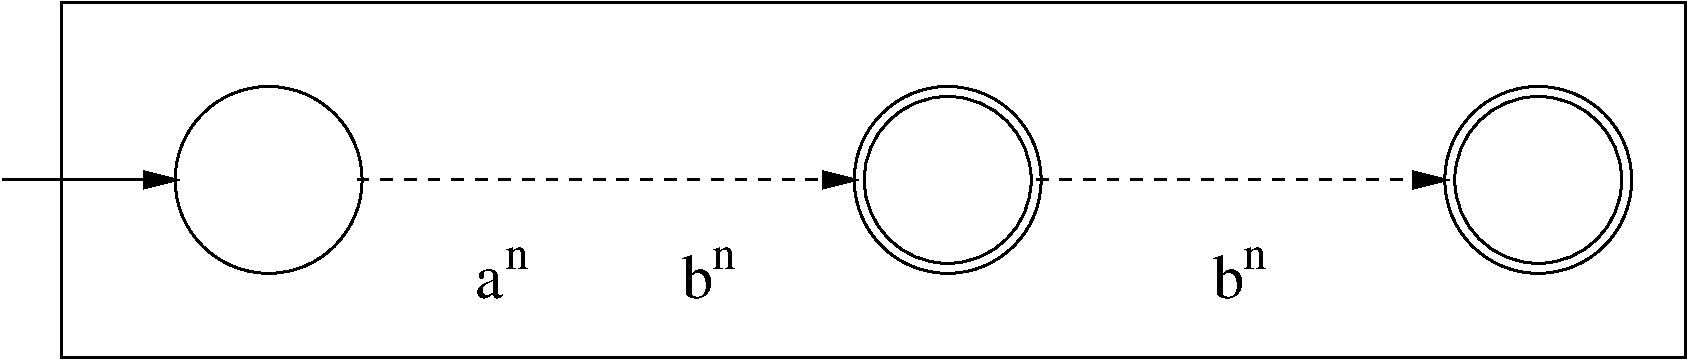
\includegraphics[%
  width=0.6\linewidth,
  keepaspectratio]{dpda1}\end{center}
\caption{The DPDA M for L\label{dpda1}}
\end{figure}

Replace in the last part of M every b by a c, and change the left
accepting state into an ordinary state. You obtain the machine in
Figure~\ref{dpda2}.
\medskip

\begin{figure}[h]
\begin{center}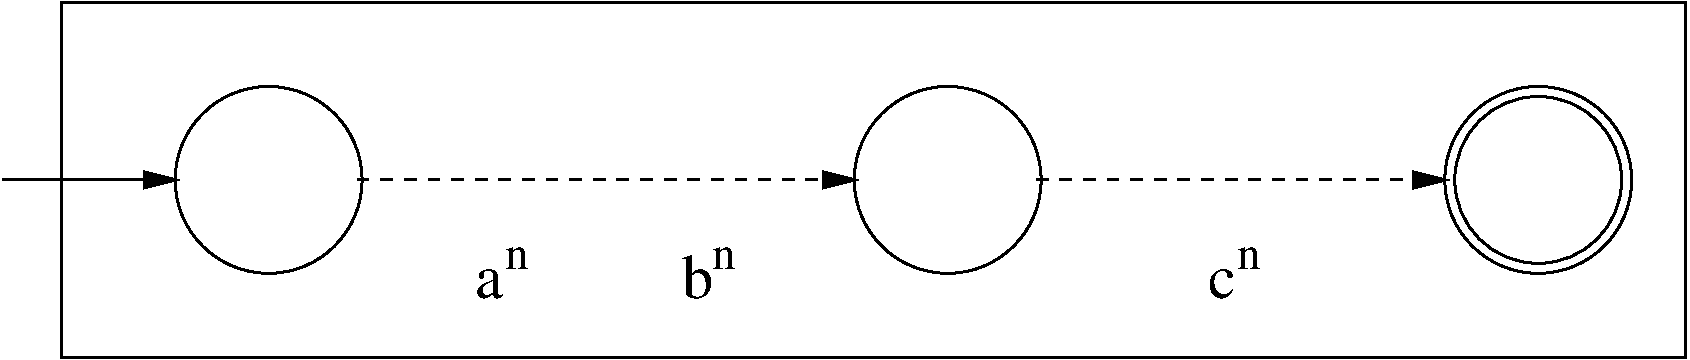
\includegraphics[%
  width=0.6\linewidth,
  keepaspectratio]{dpda2}\end{center}
\caption{The DPDA for L'\label{dpda2}}
\end{figure}

This PDA accepts $L' = \{a^nb^nc^n|n \in \N\}$ but we know already that this language is not context free!

The book by Linz contains a variant with more details.

The main reason for going into this, is that unlike for regular
languages and their FSAs, determinism makes a huge difference for
CFLs and their PDAs: one step higher in the Chomsky hierarchy,
non-determinism is suddenly very important.


\subsection{Practical Parsing Techniques}

We could be confronted with the following problem: given the
specification of a language, construct a parser for it. Perhaps this
language is the allowed input in a form to be filled out, and possibly
what you are allowed to input in a particular place depends on what
has been filled out earlier in the form. For instance, if first you
filled out you have 2 children, you should not give the names of 3
children later on. Or the language could be something with an
intricate structure, like for instance a programming language: nested
if-then-else, statement blocks, arithmetic expressions,
package qualifications ... Often this programming language is context
free, and one usually gets (or makes) the description of this language
in two levels: the first level is lexical (see page
\pageref{flexlabel}), the second level is syntactic. One uses the
BNF-notation: BNF is for Backus\footnote{Turing award in
  1977}-Naur\footnote{Turing award in 2005} form. It was used for the
first time for Algol\footnote{Look up what Algol is and how important
  it was and still is for programming language design!} \footnote{Lots
  of historical commotion: who deserves credit ... wikipedia tells you
  a lot}. BNF is very close to CFG and we already used it for the Stat
grammar on page \pageref{statlabel}.

Just as flex can produce an efficient lexer starting from a regular
expression, other tools convert a CFG to an efficient syntax
analyser. The general construction of a PDA from a CFG is not good
enough: it almost invariably results in a non-deterministic parser.
Making it deterministic is not easy, and in general even impossible as
we have found out. Therefore, these parser generators impose
some restrictions on the kind of languages/grammars they want to deal
with.

Well known parser generators are Bison (it followed Yacc) that
produces C, and ANTLER (Java). The practical use of those tools is
beyond the scope of this course, but you should know they exist, so
that if you ever need a PDA, you remember that tools can do it for
you.


The 3-state PDA we constructed from a CFG gave us leftmost topdown
derivations: the parse tree is built starting from the start symbol
downwards. One could realise that also as a deterministic program with
a {\em recursive descent parser}. It contains a number of mutually
recursive procedures that correspond to the nonterminals of the
grammar. That works only for grammars of the type {\em LL(k)}: the
$L$ means that the input is read from Left to right; the second $L$
tells us that it allows a Leftmost derivation, with $k$ symbols as
{\em look-ahead}.

There are other ways to implement a parser. Let us still read from
left to right, and stack what we read. As soon as we have read
something that matches the right side of a rule, we use that
rule. Here is a worked out example for the input $a+a*a$.


\begin{table}[ht]
\center
\begin{tabular}{|l|r|l|}
\hline
seen       & to be read      & action to take \\ \hline
           & a+a$*$a           & shift    \\
   a       &  +a$*$a           & reduce   \\
   E       &  +a$*$a           & shift    \\
   E+      &  a$*$a            & shift    \\
   E+a     &   $*$a            & reduce   \\
   E+E     &  $*$a             & reduce   \\
   E       &  $*$a             & shift    \\
   E$*$      &   a             & shift    \\
   E$*$a     &                 & reduce   \\
   E$*$E     &                 & reduce   \\
   E       &                 & stop   \\
\hline
\end{tabular}
\caption{Bottom-up parsing of $a+a*a$} \label{bottomup}
\end{table}
The actions correspond to what a shift-reduce parser does: either it
pushes the first input symbol on the stack and shifts the input
pointer one position, or it reduces what is on top of the stack, using
a grammar rule. Such a machine also needs an internal state (not shown
here) used to decide at each point which action to take. The decision
can depend on the first $k$ non-shifted input symbols as well. Such
parser constructs the rightmost parse. The corresponding grammar must
be LR(k).

Lots of research has focused on tools for the construction of
efficient parsers, e.g. for compiler front ends, for XML document
analysis ... Additionally, these tools are capable of error
correction/recovery/reporting, generation of syntax directed editors,
...  all on the basis of grammars.



% \begin{verbatim}

% Maak een CFG voor een RE

% Probeer eens een parsetree te maken voor REs

% Greibach - Kuroda - Panini ...

% BNF voor programmeerlanguages

% \end{verbatim}


\subsection{Context Sensitive Grammar}

The step from regular expressions to context free grammars involved
recursion of the nonterminals. The main restriction on a CFG was that
the left hand side of a rule could have only one symbol, a nonterminal.

The next layer of the Chomsky hierarchy belongs to the context
sensitive languages, generated by context sensitive grammars: at the
left in a rule, one may put an arbitrary string of terminals and
nonterminals: one of the nonterminals is rewritten. As an example:

$~~~~~~~~~a\underline{X}Yz$ \rpijl $a\underline{bCD}Yz$


is a context sensitive grammar rule: X can be rewritten to bCD only in
the context of an $a$ (at its left) and $Yz$ (at its right). There are
alternative, equivalent, definitions of when a rule is context
sensitive, like for instance: $\alpha$ \rpijl $\beta$ only if
$|\alpha| \leq |\beta|$.\label{altdefcs}

At first, it is not clear whether there exist context sensitive
languages that are not context free. Here is an example we studied
before: let $L = \{a^nb^nc^n|n \in \N\}$. We know already that $L$ is
not context free. But it has a context sensitive grammar (according to
the equivalent definition).

\begin{itemize}
\item[] $S$ \rpijl abc
\item[] $S$ \rpijl aSBc
\item[] cB \rpijl  Bc
\item[] bB \rpijl  bb
\end{itemize}

\paragraph{Selfie}: prove that the above grammar generates the above $L$.



There exists a normal form for context sensitive grammars: the Kuroda
normal form: each rule has one of the forms below.

\begin{itemize}
\item[] AB \rpijl CD
\item[] A \rpijl BC
\item[] A \rpijl B
\item[] A \rpijl a
\end{itemize}

A,B,C, and D are nonterminals; $a$ is any terminal.


A CSL can be parsed by a non-deterministic linear bounded automaton
(LBA). We introduce this class later: it is strictly stronger than the
PDAs. LBAs are important because they solve decision problems in
$O(n)$-space! This also indicates that there exists machinery even
stronger than LBAs!


\begin{wrapfigure}[7]{r}{.2\textwidth}
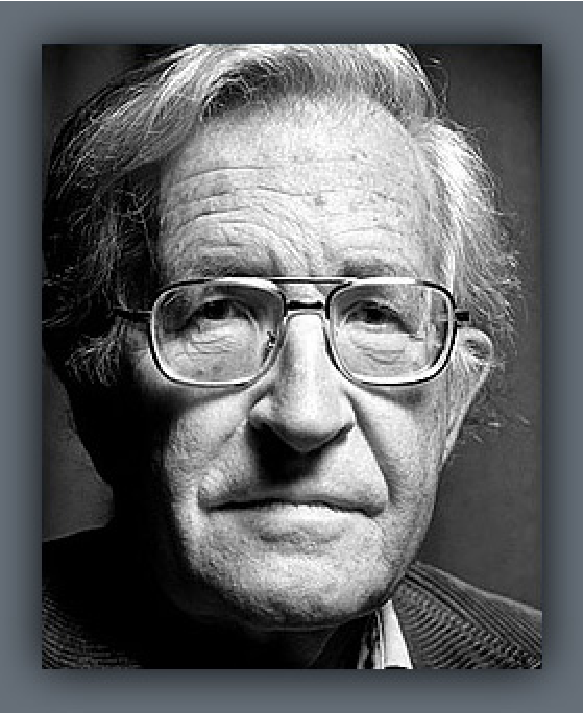
\includegraphics[width=.2\textwidth,keepaspectratio]{static/chomsky}
\end{wrapfigure}
We have almost arrived at the top of the Chomsky hierarchy: by taking
away the last restriction on the left hand side of the grammar rule,
we get the {\em unrestricted grammars}. They generate languages that
need Turing machines to be decided. They are introduced in the next
chapter.

The hierarchy can be found schematically in Table~\ref{chomskyhier}:
there exist quite a few refinements (for instance related to
determinism), but they are not shown.

~\\
~\\
\begin{table}[ht]
\center
\begin{tabular}{|l|l|l|l|}
\hline
         & Grammar          & Language              & Automaton \\ \hline
Type-0   & unrestricted        & recognisable      & Turing machine \\
Type-1   & context sensitive   & context sensitive & linear bounded   \\
Type-2   & context free        & context free      & pushdown \\
Type-3   & regular            & regular          & finite  \\
\hline
\end{tabular}
\caption{The Chomsky hierarchy} \label{chomskyhier}
\end{table}


Chomsky is also known for his political activism - it is worth to read
about it.



% \section{Een toemaatje: Stochastische Context Free Grammar}

% In een stochastische CFG (ook probabilistische CFG genoemd) wordt aan
% elke grammar rule een waarschijnlijkheid gegeven. Bijvoorbeeld:

% \begin{itemize}
% \item 0.7 Expr \rpijl Expr + Expr
% \item 0.3 Expr \rpijl Expr * Expr
% \item 1.0 Expr \rpijl a
% \end{itemize}

% Die kunnen we gebruiken om de waarschijnlijkheid van een afleiding
% te bepalen als het product van de waarschijnlijkheden van de gebruikte
% rules. Men kan dan zoeken naar de meest waarschijnlijke afleiding: in
% het geval van ambigue grammars voor natuurlijke languages geeft dat
% inzichten in wat meest waarschijnlijk bedoeld is (bijvoorbeeld als je
% aan speech recognition doet).
%

